\documentclass[]{book}
\usepackage{lmodern}
\usepackage{amssymb,amsmath}
\usepackage{ifxetex,ifluatex}
\usepackage{fixltx2e} % provides \textsubscript
\ifnum 0\ifxetex 1\fi\ifluatex 1\fi=0 % if pdftex
  \usepackage[T1]{fontenc}
  \usepackage[utf8]{inputenc}
\else % if luatex or xelatex
  \ifxetex
    \usepackage{mathspec}
  \else
    \usepackage{fontspec}
  \fi
  \defaultfontfeatures{Ligatures=TeX,Scale=MatchLowercase}
\fi
% use upquote if available, for straight quotes in verbatim environments
\IfFileExists{upquote.sty}{\usepackage{upquote}}{}
% use microtype if available
\IfFileExists{microtype.sty}{%
\usepackage{microtype}
\UseMicrotypeSet[protrusion]{basicmath} % disable protrusion for tt fonts
}{}
\usepackage[margin=1in]{geometry}
\usepackage{hyperref}
\hypersetup{unicode=true,
            pdftitle={Data Analysis and Visualization in R for Hakai Ecologists},
            pdfauthor={Data Carpentry (with modifcations)},
            pdfborder={0 0 0},
            breaklinks=true}
\urlstyle{same}  % don't use monospace font for urls
\usepackage{natbib}
\bibliographystyle{apalike}
\usepackage{color}
\usepackage{fancyvrb}
\newcommand{\VerbBar}{|}
\newcommand{\VERB}{\Verb[commandchars=\\\{\}]}
\DefineVerbatimEnvironment{Highlighting}{Verbatim}{commandchars=\\\{\}}
% Add ',fontsize=\small' for more characters per line
\usepackage{framed}
\definecolor{shadecolor}{RGB}{248,248,248}
\newenvironment{Shaded}{\begin{snugshade}}{\end{snugshade}}
\newcommand{\KeywordTok}[1]{\textcolor[rgb]{0.13,0.29,0.53}{\textbf{#1}}}
\newcommand{\DataTypeTok}[1]{\textcolor[rgb]{0.13,0.29,0.53}{#1}}
\newcommand{\DecValTok}[1]{\textcolor[rgb]{0.00,0.00,0.81}{#1}}
\newcommand{\BaseNTok}[1]{\textcolor[rgb]{0.00,0.00,0.81}{#1}}
\newcommand{\FloatTok}[1]{\textcolor[rgb]{0.00,0.00,0.81}{#1}}
\newcommand{\ConstantTok}[1]{\textcolor[rgb]{0.00,0.00,0.00}{#1}}
\newcommand{\CharTok}[1]{\textcolor[rgb]{0.31,0.60,0.02}{#1}}
\newcommand{\SpecialCharTok}[1]{\textcolor[rgb]{0.00,0.00,0.00}{#1}}
\newcommand{\StringTok}[1]{\textcolor[rgb]{0.31,0.60,0.02}{#1}}
\newcommand{\VerbatimStringTok}[1]{\textcolor[rgb]{0.31,0.60,0.02}{#1}}
\newcommand{\SpecialStringTok}[1]{\textcolor[rgb]{0.31,0.60,0.02}{#1}}
\newcommand{\ImportTok}[1]{#1}
\newcommand{\CommentTok}[1]{\textcolor[rgb]{0.56,0.35,0.01}{\textit{#1}}}
\newcommand{\DocumentationTok}[1]{\textcolor[rgb]{0.56,0.35,0.01}{\textbf{\textit{#1}}}}
\newcommand{\AnnotationTok}[1]{\textcolor[rgb]{0.56,0.35,0.01}{\textbf{\textit{#1}}}}
\newcommand{\CommentVarTok}[1]{\textcolor[rgb]{0.56,0.35,0.01}{\textbf{\textit{#1}}}}
\newcommand{\OtherTok}[1]{\textcolor[rgb]{0.56,0.35,0.01}{#1}}
\newcommand{\FunctionTok}[1]{\textcolor[rgb]{0.00,0.00,0.00}{#1}}
\newcommand{\VariableTok}[1]{\textcolor[rgb]{0.00,0.00,0.00}{#1}}
\newcommand{\ControlFlowTok}[1]{\textcolor[rgb]{0.13,0.29,0.53}{\textbf{#1}}}
\newcommand{\OperatorTok}[1]{\textcolor[rgb]{0.81,0.36,0.00}{\textbf{#1}}}
\newcommand{\BuiltInTok}[1]{#1}
\newcommand{\ExtensionTok}[1]{#1}
\newcommand{\PreprocessorTok}[1]{\textcolor[rgb]{0.56,0.35,0.01}{\textit{#1}}}
\newcommand{\AttributeTok}[1]{\textcolor[rgb]{0.77,0.63,0.00}{#1}}
\newcommand{\RegionMarkerTok}[1]{#1}
\newcommand{\InformationTok}[1]{\textcolor[rgb]{0.56,0.35,0.01}{\textbf{\textit{#1}}}}
\newcommand{\WarningTok}[1]{\textcolor[rgb]{0.56,0.35,0.01}{\textbf{\textit{#1}}}}
\newcommand{\AlertTok}[1]{\textcolor[rgb]{0.94,0.16,0.16}{#1}}
\newcommand{\ErrorTok}[1]{\textcolor[rgb]{0.64,0.00,0.00}{\textbf{#1}}}
\newcommand{\NormalTok}[1]{#1}
\usepackage{longtable,booktabs}
\usepackage{graphicx,grffile}
\makeatletter
\def\maxwidth{\ifdim\Gin@nat@width>\linewidth\linewidth\else\Gin@nat@width\fi}
\def\maxheight{\ifdim\Gin@nat@height>\textheight\textheight\else\Gin@nat@height\fi}
\makeatother
% Scale images if necessary, so that they will not overflow the page
% margins by default, and it is still possible to overwrite the defaults
% using explicit options in \includegraphics[width, height, ...]{}
\setkeys{Gin}{width=\maxwidth,height=\maxheight,keepaspectratio}
\IfFileExists{parskip.sty}{%
\usepackage{parskip}
}{% else
\setlength{\parindent}{0pt}
\setlength{\parskip}{6pt plus 2pt minus 1pt}
}
\setlength{\emergencystretch}{3em}  % prevent overfull lines
\providecommand{\tightlist}{%
  \setlength{\itemsep}{0pt}\setlength{\parskip}{0pt}}
\setcounter{secnumdepth}{5}
% Redefines (sub)paragraphs to behave more like sections
\ifx\paragraph\undefined\else
\let\oldparagraph\paragraph
\renewcommand{\paragraph}[1]{\oldparagraph{#1}\mbox{}}
\fi
\ifx\subparagraph\undefined\else
\let\oldsubparagraph\subparagraph
\renewcommand{\subparagraph}[1]{\oldsubparagraph{#1}\mbox{}}
\fi

%%% Use protect on footnotes to avoid problems with footnotes in titles
\let\rmarkdownfootnote\footnote%
\def\footnote{\protect\rmarkdownfootnote}

%%% Change title format to be more compact
\usepackage{titling}

% Create subtitle command for use in maketitle
\newcommand{\subtitle}[1]{
  \posttitle{
    \begin{center}\large#1\end{center}
    }
}

\setlength{\droptitle}{-2em}

  \title{Data Analysis and Visualization in R for Hakai Ecologists}
    \pretitle{\vspace{\droptitle}\centering\huge}
  \posttitle{\par}
    \author{Data Carpentry (with modifcations)}
    \preauthor{\centering\large\emph}
  \postauthor{\par}
      \predate{\centering\large\emph}
  \postdate{\par}
    \date{2018-12-04}

\usepackage{booktabs}

\begin{document}
\maketitle

{
\setcounter{tocdepth}{1}
\tableofcontents
}
\begin{figure}
\centering

\includegraphics{./img/DC-logo-vision.png}
\caption{}
\end{figure}

\chapter{Introduction}\label{introduction}

Data Carpentry's aim is to teach researchers basic concepts, skills, and
tools for working with data so that they can get more done in less time,
and with less pain. The lessons below were designed for those interested
in working with ecology data in R.

This is an introduction to R designed for participants with no
programming experience. These lessons can be taught in a day
(\textasciitilde{} 6 hours). They start with some basic information
about R syntax, the RStudio interface, and move through how to import
CSV files, the structure of data frames, how to deal with factors, how
to add/remove rows and columns, how to calculate summary statistics from
a data frame, and a brief introduction to plotting. The last lesson
demonstrates how to work with the Hakai database directly from R.

\section{Chapters}\label{chapters}

\begin{enumerate}
\def\labelenumi{\arabic{enumi}.}
\tightlist
\item
  \href{00-before-we-start.html}{Before we start}
\item
  \href{01-intro-to-r.html}{Introduction to R}
\item
  \href{02-starting-with-data.html}{Starting with data}
\item
  \href{03-dplyr.html}{Aggregating and analyzing data with dplyr}
\item
  \href{04-visualization-ggplot2.html}{Data visualization with
  \textbf{\texttt{ggplot2}}}
\item
  \href{05-R-api.html}{R and Databases}
\end{enumerate}

\section{Requirements}\label{requirements}

Data Carpentry's teaching is hands-on, so participants are encouraged to
use their own computers to ensure the proper setup of tools for an
efficient workflow. \emph{These lessons assume no prior knowledge of the
skills or tools}, but working through this lesson requires working
copies of the software described below. To most effectively use these
materials, please make sure to download the data and install everything
\emph{before} working through this lesson.

\subsection{Setup instructions}\label{setup-instructions}

\textbf{R} and \textbf{RStudio} are separate downloads and
installations. R is the underlying statistical computing environment,
but using R alone is no fun. RStudio is a graphical integrated
development environment (IDE) that makes using R much easier and more
interactive. You need to install R before you install RStudio. After
installing both programs, you will need to install the
\textbf{\texttt{tidyverse}} package from within RStudio. Follow the
instructions below for your operating system, and then follow the
instructions to install \textbf{\texttt{tidyverse}}.

\subsubsection{Windows}\label{windows}

\paragraph{If you already have R and RStudio
installed}\label{if-you-already-have-r-and-rstudio-installed}

\begin{itemize}
\tightlist
\item
  Open RStudio, and click on ``Help'' \textgreater{} ``Check for
  updates''. If a new version is available, quit RStudio, and download
  the latest version for RStudio.
\item
  To check which version of R you are using, start RStudio and the first
  thing that appears in the console indicates the version of R you are
  running. Alternatively, you can type \texttt{sessionInfo()}, which
  will also display which version of R you are running. Go on the
  \href{https://cran.r-project.org/bin/windows/base/}{CRAN website} and
  check whether a more recent version is available. If so, please
  download and install it. You can
  \href{https://cran.r-project.org/bin/windows/base/rw-FAQ.html\#How-do-I-UNinstall-R_003f}{check
  here} for more information on how to remove old versions from your
  system if you wish to do so.
\end{itemize}

\paragraph{If you don't have R and RStudio
installed}\label{if-you-dont-have-r-and-rstudio-installed}

\begin{itemize}
\tightlist
\item
  Download R from the
  \href{http://cran.r-project.org/bin/windows/base/release.htm}{CRAN
  website}.
\item
  Run the \texttt{.exe} file that was just downloaded
\item
  Go to the
  \href{https://www.rstudio.com/products/rstudio/download/\#download}{RStudio
  download page}
\item
  Under \emph{Installers} select \textbf{RStudio x.yy.zzz - Windows
  XP/Vista/7/8} (where x, y, and z represent version numbers)
\item
  Double click the file to install it
\item
  Once it's installed, open RStudio to make sure it works and you don't
  get any error messages.
\end{itemize}

\subsubsection{macOS}\label{macos}

\paragraph{If you already have R and RStudio
installed}\label{if-you-already-have-r-and-rstudio-installed-1}

\begin{itemize}
\tightlist
\item
  Open RStudio, and click on ``Help'' \textgreater{} ``Check for
  updates''. If a new version is available, quit RStudio, and download
  the latest version for RStudio.
\item
  To check the version of R you are using, start RStudio and the first
  thing that appears on the terminal indicates the version of R you are
  running. Alternatively, you can type \texttt{sessionInfo()}, which
  will also display which version of R you are running. Go on the
  \href{https://cran.r-project.org/bin/macosx/}{CRAN website} and check
  whether a more recent version is available. If so, please download and
  install it.
\end{itemize}

\paragraph{If you don't have R and RStudio
installed}\label{if-you-dont-have-r-and-rstudio-installed-1}

\begin{itemize}
\tightlist
\item
  Download R from the \href{http://cran.r-project.org/bin/macosx/}{CRAN
  website}.
\item
  Select the \texttt{.pkg} file for the latest R version
\item
  Double click on the downloaded file to install R
\item
  It is also a good idea to install
  \href{https://www.xquartz.org/}{XQuartz} (needed by some packages)
\item
  Go to the
  \href{https://www.rstudio.com/products/rstudio/download/\#download}{RStudio
  download page}
\item
  Under \emph{Installers} select \textbf{RStudio x.yy.zzz - Mac OS X
  10.6+ (64-bit)} (where x, y, and z represent version numbers)
\item
  Double click the file to install RStudio
\item
  Once it's installed, open RStudio to make sure it works and you don't
  get any error messages.
\end{itemize}

\subsubsection{Linux}\label{linux}

\begin{itemize}
\tightlist
\item
  Follow the instructions for your distribution from
  \href{https://cloud.r-project.org/bin/linux}{CRAN}, they provide
  information to get the most recent version of R for common
  distributions. For most distributions, you could use your package
  manager (e.g., for Debian/Ubuntu run
  \texttt{sudo\ apt-get\ install\ r-base}, and for Fedora
  \texttt{sudo\ yum\ install\ R}), but we don't recommend this approach
  as the versions provided by this are usually out of date. In any case,
  make sure you have at least R 3.3.1.
\item
  Go to the
  \href{https://www.rstudio.com/products/rstudio/download/\#download}{RStudio
  download page}
\item
  Under \emph{Installers} select the version that matches your
  distribution, and install it with your preferred method (e.g., with
  Debian/Ubuntu \texttt{sudo\ dpkg\ -i\ \ \ rstudio-x.yy.zzz-amd64.deb}
  at the terminal).
\item
  Once it's installed, open RStudio to make sure it works and you don't
  get any error messages.
\end{itemize}

\subsubsection{For everyone}\label{for-everyone}

**After installing R and RStudio, you need to install the
\texttt{tidyverse} package.

\section{Contributors}\label{contributors}

The list of contributors to this lesson is available
\href{http://datacarpentry.org/R-ecology-lesson/CITATION}{here},

Page built on: 📆 2018-12-04 ‒ 🕢 11:00:34

\chapter{Before We Start}\label{before-we-start}

\begin{center}\rule{0.5\linewidth}{\linethickness}\end{center}

\begin{quote}
\subsection{Learning Objectives}\label{learning-objectives}

\begin{itemize}
\tightlist
\item
  Describe the purpose of the RStudio Script, Console, Environment, and
  Plots panes.
\item
  Organize files and directories for a set of analyses as an R Project,
  and understand the purpose of the working directory.
\item
  Use the built-in RStudio help interface to search for more information
  on R functions.
\item
  Demonstrate how to provide sufficient information for troubleshooting
  with the R user community.
\end{itemize}
\end{quote}

\begin{center}\rule{0.5\linewidth}{\linethickness}\end{center}

\section{What is R? What is RStudio?}\label{what-is-r-what-is-rstudio}

The term ``\texttt{R}'' is used to refer to both the programming
language and the software that interprets the scripts written using it.

\href{https://rstudio.com}{RStudio} is currently a very popular way to
not only write your R scripts but also to interact with the R software.
To function correctly, RStudio needs R and therefore both need to be
installed on your computer.

\section{Why learn R?}\label{why-learn-r}

\subsection{R does not involve lots of pointing and clicking, and that's
a good
thing}\label{r-does-not-involve-lots-of-pointing-and-clicking-and-thats-a-good-thing}

The learning curve might be steeper than with other software, but with
R, the results of your analysis do not rely on remembering a succession
of pointing and clicking, but instead on a series of written commands,
and that's a good thing! So, if you want to redo your analysis because
you collected more data, you don't have to remember which button you
clicked in which order to obtain your results; you just have to run your
script again.

Working with scripts makes the steps you used in your analysis clear,
and the code you write can be inspected by someone else who can give you
feedback and spot mistakes.

Working with scripts forces you to have a deeper understanding of what
you are doing, and facilitates your learning and comprehension of the
methods you use.

\subsection{R code is great for
reproducibility}\label{r-code-is-great-for-reproducibility}

Reproducibility is when someone else (including your future self) can
obtain the same results from the same dataset when using the same
analysis.

R integrates with other tools to generate manuscripts from your code. If
you collect more data, or fix a mistake in your dataset, the figures and
the statistical tests in your manuscript are updated automatically.

An increasing number of journals and funding agencies expect analyses to
be reproducible, so knowing R will give you an edge with these
requirements.

\subsection{R is interdisciplinary and
extensible}\label{r-is-interdisciplinary-and-extensible}

With 10,000+ packages that can be installed to extend its capabilities,
R provides a framework that allows you to combine statistical approaches
from many scientific disciplines to best suit the analytical framework
you need to analyze your data. For instance, R has packages for image
analysis, GIS, time series, population genetics, and a lot more.

\subsection{R works on data of all shapes and
sizes}\label{r-works-on-data-of-all-shapes-and-sizes}

The skills you learn with R scale easily with the size of your dataset.
Whether your dataset has hundreds or millions of lines, it won't make
much difference to you.

R is designed for data analysis. It comes with special data structures
and data types that make handling of missing data and statistical
factors convenient.

R can connect to spreadsheets, databases, and many other data formats,
on your computer or on the web.

\subsection{R produces high-quality
graphics}\label{r-produces-high-quality-graphics}

The plotting functionalities in R are endless, and allow you to adjust
any aspect of your graph to convey most effectively the message from
your data.

\subsection{R has a large and welcoming
community}\label{r-has-a-large-and-welcoming-community}

Thousands of people use R daily. Many of them are willing to help you
through mailing lists and websites such as
\href{https://stackoverflow.com/}{Stack Overflow}, or on the
\href{https://community.rstudio.com/}{RStudio community}.

\subsection{Not only is R free, but it is also open-source and
cross-platform}\label{not-only-is-r-free-but-it-is-also-open-source-and-cross-platform}

Anyone can inspect the source code to see how R works. Because of this
transparency, there is less chance for mistakes, and if you (or someone
else) find some, you can report and fix bugs.

\section{Knowing your way around
RStudio}\label{knowing-your-way-around-rstudio}

Let's start by learning about \href{https://www.rstudio.com/}{RStudio},
which is an Integrated Development Environment (IDE) for working with R.

The RStudio IDE open-source product is free under the
\href{https://www.gnu.org/licenses/agpl-3.0.en.html}{Affero General
Public License (AGPL) v3}. The RStudio IDE is also available with a
commercial license and priority email support from RStudio, Inc.

We will use RStudio IDE to write code, navigate the files on our
computer, inspect the variables we are going to create, and visualize
the plots we will generate. RStudio can also be used for other things
(e.g., version control, developing packages, writing Shiny apps) that we
will not cover during the workshop.

\begin{figure}
\centering
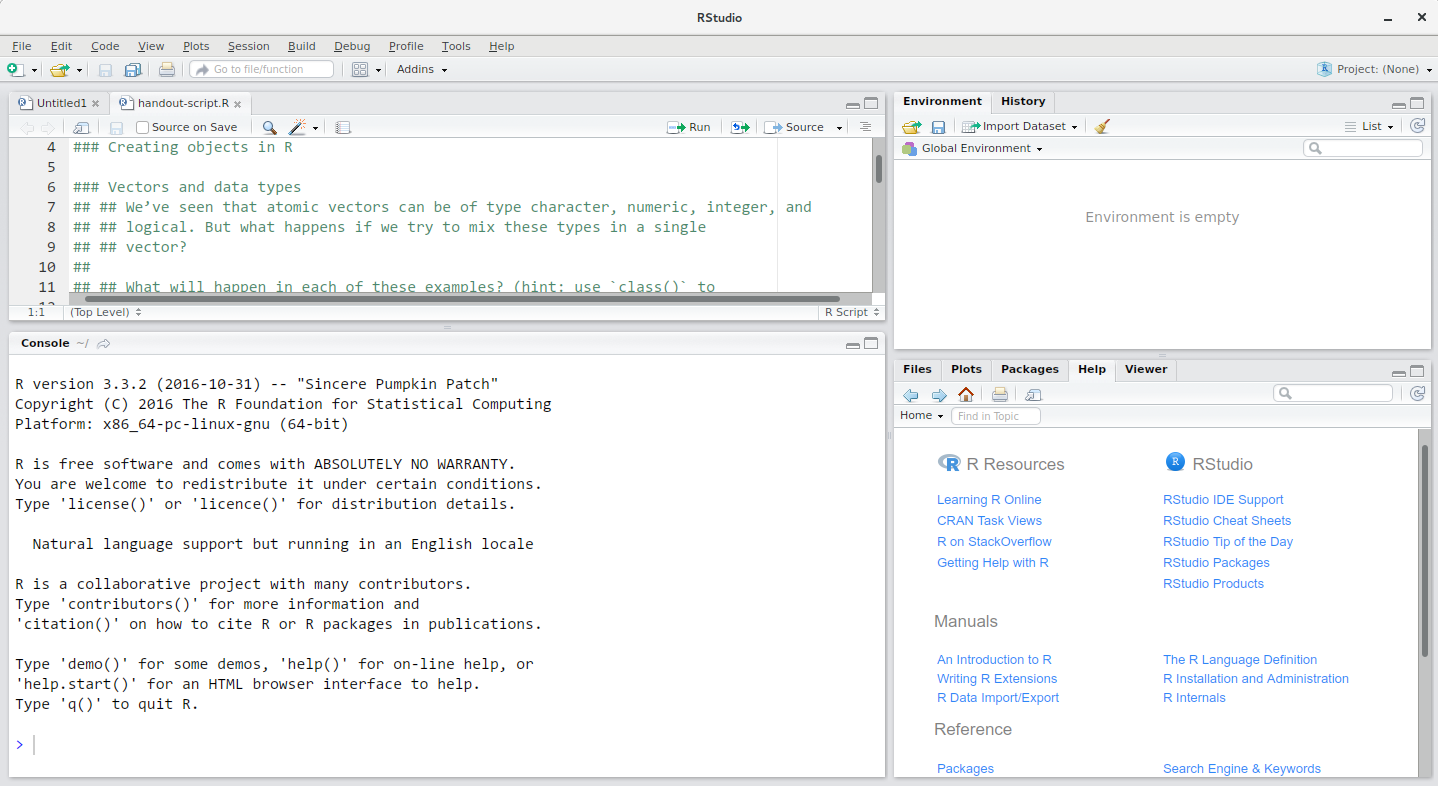
\includegraphics{img/rstudio-screenshot.png}
\caption{RStudio interface screenshot. Clockwise from top left: Source,
Environment/History, Files/Plots/Packages/Help/Viewer, Console.}
\end{figure}

RStudio is divided into 4 ``Panes'': the \textbf{Source} for your
scripts and documents (top-left, in the default layout), your
\textbf{Environment/History} (top-right), your
\textbf{Files/Plots/Packages/Help/Viewer} (bottom-right), and the R
\textbf{Console} (bottom-left). The placement of these panes and their
content can be customized (see menu, Tools -\textgreater{} Global
Options -\textgreater{} Pane Layout).

One of the advantages of using RStudio is that all the information you
need to write code is available in a single window. Additionally, with
many shortcuts, autocompletion, and highlighting for the major file
types you use while developing in R, RStudio will make typing easier and
less error-prone.

\section{Getting set up}\label{getting-set-up}

It is good practice to keep a set of related data, analyses, and text
self-contained in a single folder, called the \textbf{working
directory}. All of the scripts within this folder can then use
\emph{relative paths} to files that indicate where inside the project a
file is located (as opposed to absolute paths, which point to where a
file is on a specific computer). Working this way makes it a lot easier
to move your project around on your computer and share it with others
without worrying about whether or not the underlying scripts will still
work.

RStudio provides a helpful set of tools to do this through its
``Projects'' interface, which not only creates a working directory for
you, but also remembers its location (allowing you to quickly navigate
to it) and optionally preserves custom settings and open files to make
it easier to resume work after a break. Go through the steps for
creating an ``R Project'' for this tutorial below.

\begin{enumerate}
\def\labelenumi{\arabic{enumi}.}
\tightlist
\item
  Start RStudio.
\item
  Under the \texttt{File} menu, click on \texttt{New\ project}. Choose
  \texttt{New\ directory}, then \texttt{New\ project}.
\item
  Enter a name for this new folder (or ``directory''), and choose a
  convenient location for it. This will be your \textbf{working
  directory} for the rest of the day (e.g.,
  \texttt{\textasciitilde{}/intro\_to\_r}).
\item
  Click on \texttt{Create\ project}.
\item
  Download
  \href{https://drive.google.com/file/d/1GnrIlrcxDUmlVm40Tx9LawfxaeSh5Mu1/view?usp=sharing}{this
  file} and put it in a new folder in your \texttt{intro\_to\_r} folder
  and call the new folder \texttt{data\_output}
\item
  Set Preferences to `Never' save workspace in RStudio.
\end{enumerate}

RStudio's default preferences generally work well, but saving a
workspace to .RData can be cumbersome, especially if you are working
with larger datasets. To turn that off, go to Tools --\textgreater{}
`Global Options' and select the `Never' option for `Save workspace to
.RData' on exit.'

\begin{figure}
\centering
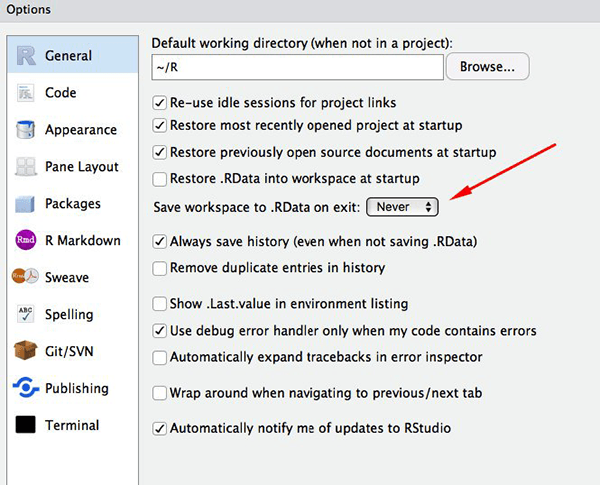
\includegraphics{img/rstudio-preferences.png}
\caption{Set `Save workspace to .RData on exit' to `Never'}
\end{figure}

\subsection{Organizing your working
directory}\label{organizing-your-working-directory}

Using a consistent folder structure across your projects will help keep
things organized, and will also make it easy to find/file things in the
future. This can be especially helpful when you have multiple projects.
In general, you may create directories (folders) for \textbf{scripts},
\textbf{data}, and \textbf{documents}.

\begin{itemize}
\tightlist
\item
  \textbf{\texttt{data/}} Use this folder to store your raw data and
  intermediate datasets you may create for the need of a particular
  analysis. For the sake of transparency and
  \href{https://en.wikipedia.org/wiki/Provenance}{provenance}, you
  should \emph{always} keep a copy of your raw data accessible and do as
  much of your data cleanup and preprocessing programmatically (i.e.,
  with scripts, rather than manually) as possible. Separating raw data
  from processed data is also a good idea. For example, you could have
  files \texttt{data/raw/tree\_survey.plot1.txt} and
  \texttt{...plot2.txt} kept separate from a
  \texttt{data/processed/tree.survey.csv} file generated by the
  \texttt{scripts/01.preprocess.tree\_survey.R} script.
\item
  \textbf{\texttt{documents/}} This would be a place to keep outlines,
  drafts, and other text.
\item
  \textbf{\texttt{scripts/}} This would be the location to keep your R
  scripts for different analyses or plotting, and potentially a separate
  folder for your functions (more on that later).
\end{itemize}

You may want additional directories or subdirectories depending on your
project needs, but these should form the backbone of your working
directory.

\begin{figure}
\centering
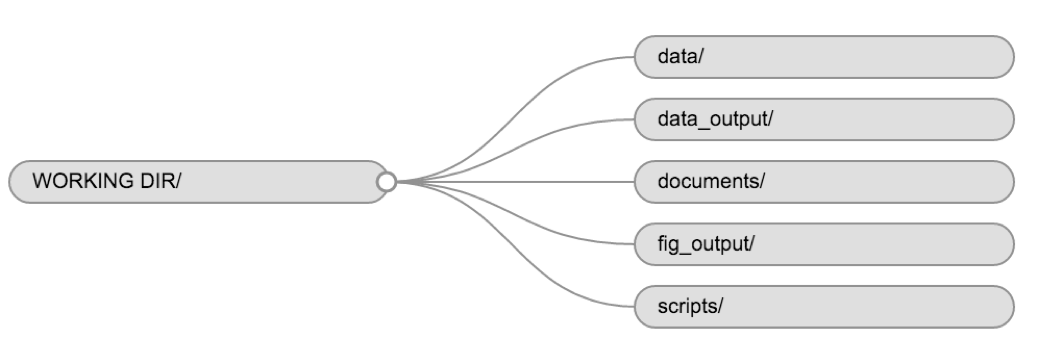
\includegraphics{img/working-directory-structure.png}
\caption{Example of a working directory structure.}
\end{figure}

For this workshop, we will need a \texttt{data/} folder to store our raw
data, and we will use \texttt{data\_output/} for when we learn how to
export data as CSV files, and \texttt{fig\_output/} folder for the
figures that we will save.

\begin{itemize}
\tightlist
\item
  Under the \texttt{Files} tab on the right of the screen, click on
  \texttt{New\ Folder} and create a folder named \texttt{data} within
  your newly created working directory (e.g.,
  \texttt{\textasciitilde{}/data-carpentry/data}). (Alternatively, type
  \texttt{dir.create("data")} at your R console.) Repeat these
  operations to create a \texttt{data\_output/} and a
  \texttt{fig\_output} folders.
\end{itemize}

We are going to keep the script in the root of our working directory
because we are only going to use one file and it will make things
easier.

Your working directory should now look like this:

\begin{figure}

{\centering 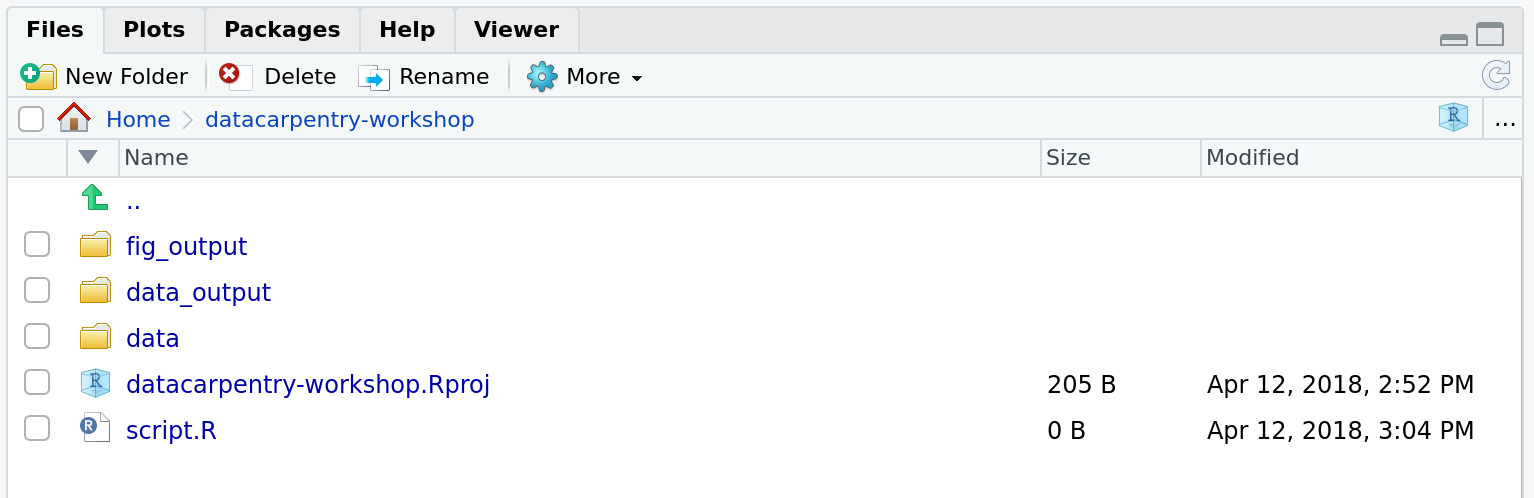
\includegraphics[width=1\linewidth]{img/r-starting-how-it-should-look-like} 

}

\caption{How it should look like at the beginning of this lesson}\label{fig:unnamed-chunk-3}
\end{figure}

\subsection{The working directory}\label{the-working-directory}

The working directory is an important concept to understand. It is the
place from where R will be looking for and saving the files. When you
write code for your project, it should refer to files in relation to the
root of your working directory and only need files within this
structure.

Using RStudio projects makes this easy and ensures that your working
directory is set properly. If you need to check it, you can use
\texttt{getwd()}. If for some reason your working directory is not what
it should be, you can change it in the RStudio interface by navigating
in the file browser where your working directory should be, and clicking
on the blue gear icon ``More'', and select ``Set As Working Directory''.
Alternatively you can use \texttt{setwd("/path/to/working/directory")}
to reset your working directory. However, your scripts should not
include this line because it will fail on someone else's computer.

\section{Interacting with R}\label{interacting-with-r}

The basis of programming is that we write down instructions for the
computer to follow, and then we tell the computer to follow those
instructions. We write, or \emph{code}, instructions in R because it is
a common language that both the computer and we can understand. We call
the instructions \emph{commands} and we tell the computer to follow the
instructions by \emph{executing} (also called \emph{running}) those
commands.

There are two main ways of interacting with R: by using the console or
by using script files (plain text files that contain your code). The
console pane (in RStudio, the bottom left panel) is the place where
commands written in the R language can be typed and executed immediately
by the computer. It is also where the results will be shown for commands
that have been executed. You can type commands directly into the console
and press \texttt{Enter} to execute those commands, but they will be
forgotten when you close the session.

Because we want our code and workflow to be reproducible, it is better
to type the commands we want in the script editor, and save the script.
This way, there is a complete record of what we did, and anyone
(including our future selves!) can easily replicate the results on their
computer.

RStudio allows you to execute commands directly from the script editor
by using the \texttt{Ctrl} + \texttt{Enter} shortcut (on Macs,
\texttt{Cmd} + \texttt{Return} will work, too). The command on the
current line in the script (indicated by the cursor) or all of the
commands in the currently selected text will be sent to the console and
executed when you press \texttt{Ctrl} + \texttt{Enter}. You can find
other keyboard shortcuts in this
\href{https://github.com/rstudio/cheatsheets/raw/master/rstudio-ide.pdf}{RStudio
cheatsheet about the RStudio IDE}.

At some point in your analysis you may want to check the content of a
variable or the structure of an object, without necessarily keeping a
record of it in your script. You can type these commands and execute
them directly in the console. RStudio provides the \texttt{Ctrl} +
\texttt{1} and \texttt{Ctrl} + \texttt{2} shortcuts allow you to jump
between the script and the console panes.

If R is ready to accept commands, the R console shows a
\texttt{\textgreater{}} prompt. If it receives a command (by typing,
copy-pasting or sent from the script editor using \texttt{Ctrl} +
\texttt{Enter}), R will try to execute it, and when ready, will show the
results and come back with a new \texttt{\textgreater{}} prompt to wait
for new commands.

If R is still waiting for you to enter more data because it isn't
complete yet, the console will show a \texttt{+} prompt. It means that
you haven't finished entering a complete command. This is because you
have not `closed' a parenthesis or quotation, i.e.~you don't have the
same number of left-parentheses as right-parentheses, or the same number
of opening and closing quotation marks. When this happens, and you
thought you finished typing your command, click inside the console
window and press \texttt{Esc}; this will cancel the incomplete command
and return you to the \texttt{\textgreater{}} prompt.

\section{How to learn more after the
workshop?}\label{how-to-learn-more-after-the-workshop}

The material we cover during this workshop will give you an initial
taste of how you can use R to analyze data for your own research.
However, you will need to learn more to do advanced operations such as
cleaning your dataset, using statistical methods, or creating beautiful
graphics. The best way to become proficient and efficient at R, as with
any other tool, is to use it to address your actual research questions.
As a beginner, it can feel daunting to have to write a script from
scratch, and given that many people make their code available online,
modifying existing code to suit your purpose might make it easier for
you to get started.

\section{Seeking help}\label{seeking-help}

\subsection{Use the built-in RStudio help interface to search for more
information on R
functions}\label{use-the-built-in-rstudio-help-interface-to-search-for-more-information-on-r-functions}

\begin{figure}
\centering
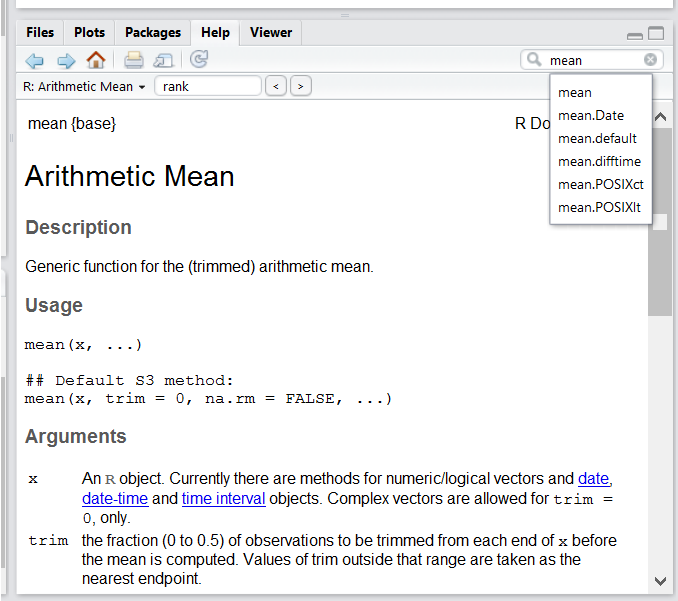
\includegraphics{img/rstudiohelp.png}
\caption{RStudio help interface.}
\end{figure}

One of the fastest ways to get help, is to use the RStudio help
interface. This panel by default can be found at the lower right hand
panel of RStudio. As seen in the screenshot, by typing the word
``Mean'', RStudio tries to also give a number of suggestions that you
might be interested in. The description is then shown in the display
window.

\subsection{I know the name of the function I want to use, but I'm not
sure how to use
it}\label{i-know-the-name-of-the-function-i-want-to-use-but-im-not-sure-how-to-use-it}

If you need help with a specific function, let's say \texttt{barplot()},
you can type:

\begin{Shaded}
\begin{Highlighting}[]
\NormalTok{?barplot}
\end{Highlighting}
\end{Shaded}

If you just need to remind yourself of the names of the arguments, you
can use:

\begin{Shaded}
\begin{Highlighting}[]
\KeywordTok{args}\NormalTok{(lm)}
\end{Highlighting}
\end{Shaded}

\subsection{I want to use a function that does X, there must be a
function for it but I don't know which
one\ldots{}}\label{i-want-to-use-a-function-that-does-x-there-must-be-a-function-for-it-but-i-dont-know-which-one}

If you are looking for a function to do a particular task, you can use
the \texttt{help.search()} function, which is called by the double
question mark \texttt{??}. However, this only looks through the
installed packages for help pages with a match to your search request

\begin{Shaded}
\begin{Highlighting}[]
\NormalTok{??kruskal}
\end{Highlighting}
\end{Shaded}

If you can't find what you are looking for, you can use the
\href{http://www.rdocumentation.org}{rdocumentation.org} website that
searches through the help files across all packages available.

Finally, a generic Google or internet search ``R
\textless{}task\textgreater{}'' will often either send you to the
appropriate package documentation or a helpful forum where someone else
has already asked your question.

\subsection{I am stuck\ldots{} I get an error message that I don't
understand}\label{i-am-stuck-i-get-an-error-message-that-i-dont-understand}

Start by googling the error message. However, this doesn't always work
very well because often, package developers rely on the error catching
provided by R. You end up with general error messages that might not be
very helpful to diagnose a problem (e.g. ``subscript out of bounds'').
If the message is very generic, you might also include the name of the
function or package you're using in your query.

However, you should check Stack Overflow. Search using the
\texttt{{[}r{]}} tag. Most questions have already been answered, but the
challenge is to use the right words in the search to find the answers:
\url{http://stackoverflow.com/questions/tagged/r}

\subsection{More resources}\label{more-resources}

\begin{itemize}
\tightlist
\item
  The \href{https://community.rstudio.com/}{R-Studio Community Forums}
\item
  \href{http://r4ds.had.co.nz}{R for Data Science}
\item
  Stack Overflow
\item
  \href{http://hecate.hakai.org/rguide}{Hakai R Guide for Reproducible
  Analyses}
\end{itemize}

\chapter{Intro to R}\label{intro-to-r}

\begin{center}\rule{0.5\linewidth}{\linethickness}\end{center}

\begin{quote}
\subsection{Learning Objectives}\label{learning-objectives-1}

\begin{itemize}
\tightlist
\item
  Define the following terms as they relate to R: object, assign, call,
  function, arguments, options.
\item
  Assign values to objects in R.
\item
  Learn how to \emph{name} objects
\item
  Use comments to inform script.
\item
  Solve simple arithmetic operations in R.
\item
  Call functions and use arguments to change their default options.
\item
  Inspect the content of vectors and manipulate their content.
\item
  Subset and extract values from vectors.
\item
  Analyze vectors with missing data.
\end{itemize}
\end{quote}

\begin{center}\rule{0.5\linewidth}{\linethickness}\end{center}

\section{Creating objects in R}\label{creating-objects-in-r}

You can get output from R simply by typing math in the console:

\begin{Shaded}
\begin{Highlighting}[]
\DecValTok{3} \OperatorTok{+}\StringTok{ }\DecValTok{5}
\DecValTok{12} \OperatorTok{/}\StringTok{ }\DecValTok{7}
\end{Highlighting}
\end{Shaded}

However, to do useful and interesting things, we need to assign
\emph{values} to \emph{objects}. To create an object, we need to give it
a name followed by the assignment operator \texttt{\textless{}-}, and
the value we want to give it:

\begin{Shaded}
\begin{Highlighting}[]
\NormalTok{weight_kg <-}\StringTok{ }\DecValTok{55}
\end{Highlighting}
\end{Shaded}

\texttt{\textless{}-} is the assignment operator. It assigns values on
the right to objects on the left. So, after executing
\texttt{x\ \textless{}-\ 3}, the value of \texttt{x} is \texttt{3}. The
arrow can be read as 3 \textbf{goes into} \texttt{x}. For historical
reasons, you can also use \texttt{=} for assignments, but not in every
context. Because of the
\href{http://blog.revolutionanalytics.com/2008/12/use-equals-or-arrow-for-assignment.html}{slight}
\href{http://r.789695.n4.nabble.com/Is-there-any-difference-between-and-tp878594p878598.html}{differences}
in syntax, it is good practice to always use \texttt{\textless{}-} for
assignments.

In RStudio, typing Alt + - (push Alt at the same time as the - key) will
write \texttt{\textless{}-} in a single keystroke in a PC, while typing
Option + - (push Option at the same time as the - key) does the same in
a Mac.

Objects can be given any name such as \texttt{x},
\texttt{current\_temperature}, or \texttt{subject\_id}. You want your
object names to be explicit and not too long. They cannot start with a
number (\texttt{2x} is not valid, but \texttt{x2} is). R is case
sensitive (e.g., \texttt{weight\_kg} is different from
\texttt{Weight\_kg}). There are some names that cannot be used because
they are the names of fundamental functions in R (e.g., \texttt{if},
\texttt{else}, \texttt{for}, see
\href{https://stat.ethz.ch/R-manual/R-devel/library/base/html/Reserved.html}{here}
for a complete list). In general, even if it's allowed, it's best to not
use other function names (e.g., \texttt{c}, \texttt{T}, \texttt{mean},
\texttt{data}, \texttt{df}, \texttt{weights}). If in doubt, check the
help to see if the name is already in use. It's also best to avoid dots
(\texttt{.}) within an object name as in \texttt{my.dataset}. There are
many functions in R with dots in their names for historical reasons, but
because dots have a special meaning in R (for methods) and other
programming languages, it's best to avoid them. It is also recommended
to use nouns for object names, and verbs for function names. It's
important to be consistent in the styling of your code (where you put
spaces, how you name objects, etc.). Using a consistent coding style
makes your code clearer to read for your future self and your
collaborators. In R, the best style guide is the
\href{http://style.tidyverse.org/}{tidyverse's}. The tidyverse's is very
comprehensive and may seem overwhelming at first. You can install the
\href{https://github.com/jimhester/lintr}{\textbf{\texttt{lintr}}}
package to automatically check for issues in the styling of your code.

\begin{quote}
\subsection{Objects vs.~variables}\label{objects-vs.variables}

What are known as \texttt{objects} in \texttt{R} are known as
\texttt{variables} in many other programming languages. Depending on the
context, \texttt{object} and \texttt{variable} can have drastically
different meanings. However, in this lesson, the two words are used
synonymously. For more information see:
\url{https://cran.r-project.org/doc/manuals/r-release/R-lang.html\#Objects}
\end{quote}

When assigning a value to an object, R does not print anything. You can
force R to print the value by using parentheses or by typing the object
name:

\begin{Shaded}
\begin{Highlighting}[]
\NormalTok{weight_kg <-}\StringTok{ }\DecValTok{55}    \CommentTok{# doesn't print anything}
\NormalTok{(weight_kg <-}\StringTok{ }\DecValTok{55}\NormalTok{)  }\CommentTok{# but putting parenthesis around the call prints the value of `weight_kg`}
\NormalTok{weight_kg          }\CommentTok{# and so does typing the name of the object}
\end{Highlighting}
\end{Shaded}

Now that R has \texttt{weight\_kg} in memory, we can do arithmetic with
it. For instance, we may want to convert this weight into pounds (weight
in pounds is 2.2 times the weight in kg):

\begin{Shaded}
\begin{Highlighting}[]
\FloatTok{2.2} \OperatorTok{*}\StringTok{ }\NormalTok{weight_kg}
\end{Highlighting}
\end{Shaded}

We can also change an object's value by assigning it a new one:

\begin{Shaded}
\begin{Highlighting}[]
\NormalTok{weight_kg <-}\StringTok{ }\FloatTok{57.5}
\FloatTok{2.2} \OperatorTok{*}\StringTok{ }\NormalTok{weight_kg}
\end{Highlighting}
\end{Shaded}

This means that assigning a value to one object does not change the
values of other objects For example, let's store the animal's weight in
pounds in a new object, \texttt{weight\_lb}:

\begin{Shaded}
\begin{Highlighting}[]
\NormalTok{weight_lb <-}\StringTok{ }\FloatTok{2.2} \OperatorTok{*}\StringTok{ }\NormalTok{weight_kg}
\end{Highlighting}
\end{Shaded}

and then change \texttt{weight\_kg} to 100.

\begin{Shaded}
\begin{Highlighting}[]
\NormalTok{weight_kg <-}\StringTok{ }\DecValTok{100}
\end{Highlighting}
\end{Shaded}

What do you think is the current content of the object
\texttt{weight\_lb}? 126.5 or 220?

\subsection{Comments}\label{comments}

The comment character in R is \texttt{\#}, anything to the right of a
\texttt{\#} in a script will be ignored by R. It is useful to leave
notes, and explanations in your scripts. RStudio makes it easy to
comment or uncomment a paragraph: after selecting the lines you want to
comment, press at the same time on your keyboard Ctrl + Shift + C. If
you only want to comment out one line, you can put the cursor at any
location of that line (i.e.~no need to select the whole line), then
press Ctrl + Shift + C.

\begin{quote}
\subsection{Challenge}\label{challenge}

What are the values after each statement in the following?

\begin{Shaded}
\begin{Highlighting}[]
\NormalTok{mass <-}\StringTok{ }\FloatTok{47.5}            \CommentTok{# mass?}
\NormalTok{age  <-}\StringTok{ }\DecValTok{122}             \CommentTok{# age?}
\NormalTok{mass <-}\StringTok{ }\NormalTok{mass }\OperatorTok{*}\StringTok{ }\FloatTok{2.0}      \CommentTok{# mass?}
\NormalTok{age  <-}\StringTok{ }\NormalTok{age }\OperatorTok{-}\StringTok{ }\DecValTok{20}        \CommentTok{# age?}
\NormalTok{mass_index <-}\StringTok{ }\NormalTok{mass}\OperatorTok{/}\NormalTok{age  }\CommentTok{# mass_index?}
\end{Highlighting}
\end{Shaded}
\end{quote}

\subsection{Functions and their
arguments}\label{functions-and-their-arguments}

Functions are ``canned scripts'' that automate more complicated sets of
commands including operations assignments, etc. Many functions are
predefined, or can be made available by importing R \emph{packages}
(more on that later). A function usually gets one or more inputs called
\emph{arguments}. Functions often (but not always) return a
\emph{value}. A typical example would be the function \texttt{sqrt()}.
The input (the argument) must be a number, and the return value (in
fact, the output) is the square root of that number. Executing a
function (`running it') is called \emph{calling} the function. An
example of a function call is:

\begin{Shaded}
\begin{Highlighting}[]
\NormalTok{b <-}\StringTok{ }\KeywordTok{sqrt}\NormalTok{(a)}
\end{Highlighting}
\end{Shaded}

Here, the value of \texttt{a} is given to the \texttt{sqrt()} function,
the \texttt{sqrt()} function calculates the square root, and returns the
value which is then assigned to the object \texttt{b}. This function is
very simple, because it takes just one argument.

The return `value' of a function need not be numerical (like that of
\texttt{sqrt()}), and it also does not need to be a single item: it can
be a set of things, or even a dataset. We'll see that when we read data
files into R.

Arguments can be anything, not only numbers or filenames, but also other
objects. Exactly what each argument means differs per function, and must
be looked up in the documentation (see below). Some functions take
arguments which may either be specified by the user, or, if left out,
take on a \emph{default} value: these are called \emph{options}. Options
are typically used to alter the way the function operates, such as
whether it ignores `bad values', or what symbol to use in a plot.
However, if you want something specific, you can specify a value of your
choice which will be used instead of the default.

Let's try a function that can take multiple arguments: \texttt{round()}.

\begin{Shaded}
\begin{Highlighting}[]
\KeywordTok{round}\NormalTok{(}\FloatTok{3.14159}\NormalTok{)}
\end{Highlighting}
\end{Shaded}

\begin{verbatim}
#> [1] 3
\end{verbatim}

Here, we've called \texttt{round()} with just one argument,
\texttt{3.14159}, and it has returned the value \texttt{3}. That's
because the default is to round to the nearest whole number. If we want
more digits we can see how to do that by getting information about the
\texttt{round} function. We can use \texttt{args(round)} or look at the
help for this function using \texttt{?round}.

\begin{Shaded}
\begin{Highlighting}[]
\KeywordTok{args}\NormalTok{(round)}
\end{Highlighting}
\end{Shaded}

\begin{verbatim}
#> function (x, digits = 0) 
#> NULL
\end{verbatim}

\begin{Shaded}
\begin{Highlighting}[]
\NormalTok{?round}
\end{Highlighting}
\end{Shaded}

We see that if we want a different number of digits, we can type
\texttt{digits=2} or however many we want.

\begin{Shaded}
\begin{Highlighting}[]
\KeywordTok{round}\NormalTok{(}\FloatTok{3.14159}\NormalTok{, }\DataTypeTok{digits =} \DecValTok{2}\NormalTok{)}
\end{Highlighting}
\end{Shaded}

\begin{verbatim}
#> [1] 3.14
\end{verbatim}

If you provide the arguments in the exact same order as they are defined
you don't have to name them:

\begin{Shaded}
\begin{Highlighting}[]
\KeywordTok{round}\NormalTok{(}\FloatTok{3.14159}\NormalTok{, }\DecValTok{2}\NormalTok{)}
\end{Highlighting}
\end{Shaded}

\begin{verbatim}
#> [1] 3.14
\end{verbatim}

And if you do name the arguments, you can switch their order:

\begin{Shaded}
\begin{Highlighting}[]
\KeywordTok{round}\NormalTok{(}\DataTypeTok{digits =} \DecValTok{2}\NormalTok{, }\DataTypeTok{x =} \FloatTok{3.14159}\NormalTok{)}
\end{Highlighting}
\end{Shaded}

\begin{verbatim}
#> [1] 3.14
\end{verbatim}

It's good practice to put the non-optional arguments (like the number
you're rounding) first in your function call, and to specify the names
of all optional arguments. If you don't, someone reading your code might
have to look up the definition of a function with unfamiliar arguments
to understand what you're doing.

\section{Vectors and data types}\label{vectors-and-data-types}

A vector is the most common and basic data type in R, and is pretty much
the workhorse of R. A vector is composed by a series of values, which
can be either numbers or characters. We can assign a series of values to
a vector using the \texttt{c()} function. For example we can create a
vector of animal weights and assign it to a new object
\texttt{weight\_g}:

\begin{Shaded}
\begin{Highlighting}[]
\NormalTok{weight_g <-}\StringTok{ }\KeywordTok{c}\NormalTok{(}\DecValTok{50}\NormalTok{, }\DecValTok{60}\NormalTok{, }\DecValTok{65}\NormalTok{, }\DecValTok{82}\NormalTok{)}
\NormalTok{weight_g}
\end{Highlighting}
\end{Shaded}

A vector can also contain characters:

\begin{Shaded}
\begin{Highlighting}[]
\NormalTok{animals <-}\StringTok{ }\KeywordTok{c}\NormalTok{(}\StringTok{"mouse"}\NormalTok{, }\StringTok{"rat"}\NormalTok{, }\StringTok{"dog"}\NormalTok{)}
\NormalTok{animals}
\end{Highlighting}
\end{Shaded}

Mouse, rat and dog are called elements of the animals vector. The quotes
around ``mouse'', ``rat'', etc. are essential here. Without the quotes R
will assume there are objects called \texttt{mouse}, \texttt{rat} and
\texttt{dog}. As these objects don't exist in R's memory, there will be
an error message.

There are many functions that allow you to inspect the content of a
vector. \texttt{length()} tells you how many elements are in a
particular vector:

\begin{Shaded}
\begin{Highlighting}[]
\KeywordTok{length}\NormalTok{(weight_g)}
\KeywordTok{length}\NormalTok{(animals)}
\end{Highlighting}
\end{Shaded}

An important feature of a vector, is that all of the elements are the
same type of data. The function \texttt{class()} indicates the class
(the type of element) of an object:

\begin{Shaded}
\begin{Highlighting}[]
\KeywordTok{class}\NormalTok{(weight_g)}
\KeywordTok{class}\NormalTok{(animals)}
\end{Highlighting}
\end{Shaded}

An \textbf{atomic vector} is the simplest R \textbf{data type} and is a
linear vector of a single type. Above, we saw 2 of the 6 main
\textbf{atomic vector} types that R uses: \texttt{"character"} and
\texttt{"numeric"} (or \texttt{"double"}). These are the basic building
blocks that all R objects are built from. The other 4 \textbf{atomic
vector} types are:

\begin{itemize}
\tightlist
\item
  \texttt{"logical"} for \texttt{TRUE} and \texttt{FALSE} (the boolean
  data type)
\item
  \texttt{"integer"} for integer numbers (e.g., \texttt{2L}, the
  \texttt{L} indicates to R that it's an integer)
\item
  \texttt{"complex"} to represent complex numbers with real and
  imaginary parts (e.g., \texttt{1\ +\ 4i}) and that's all we're going
  to say about them
\item
  \texttt{"raw"} for bitstreams that we won't discuss further
\end{itemize}

You can check the type of your vector using the \texttt{typeof()}
function and inputting your vector as the argument.

Vectors are one of the many \textbf{data structures} that R uses. Other
important ones are lists (\texttt{list}), matrices (\texttt{matrix}),
data frames (\texttt{data.frame}), factors (\texttt{factor}) and arrays
(\texttt{array}).

\begin{quote}
\subsection{Challenge}\label{challenge-1}

\begin{itemize}
\item
  We've seen that atomic vectors can be of type character, numeric (or
  double), integer, and logical. But what happens if we try to mix these
  types in a single vector?
\item
  What will happen in each of these examples? (hint: use
  \texttt{class()} to check the data type of your objects):

\begin{Shaded}
\begin{Highlighting}[]
\NormalTok{num_char <-}\StringTok{ }\KeywordTok{c}\NormalTok{(}\DecValTok{1}\NormalTok{, }\DecValTok{2}\NormalTok{, }\DecValTok{3}\NormalTok{, }\StringTok{"a"}\NormalTok{)}
\NormalTok{num_logical <-}\StringTok{ }\KeywordTok{c}\NormalTok{(}\DecValTok{1}\NormalTok{, }\DecValTok{2}\NormalTok{, }\DecValTok{3}\NormalTok{, }\OtherTok{TRUE}\NormalTok{)}
\NormalTok{char_logical <-}\StringTok{ }\KeywordTok{c}\NormalTok{(}\StringTok{"a"}\NormalTok{, }\StringTok{"b"}\NormalTok{, }\StringTok{"c"}\NormalTok{, }\OtherTok{TRUE}\NormalTok{)}
\NormalTok{tricky <-}\StringTok{ }\KeywordTok{c}\NormalTok{(}\DecValTok{1}\NormalTok{, }\DecValTok{2}\NormalTok{, }\DecValTok{3}\NormalTok{, }\StringTok{"4"}\NormalTok{)}
\end{Highlighting}
\end{Shaded}
\item
  Why do you think it happens?
\item
  How many values in \texttt{combined\_logical} are \texttt{"TRUE"} (as
  a character) in the following example:

\begin{Shaded}
\begin{Highlighting}[]
\NormalTok{num_logical <-}\StringTok{ }\KeywordTok{c}\NormalTok{(}\DecValTok{1}\NormalTok{, }\DecValTok{2}\NormalTok{, }\DecValTok{3}\NormalTok{, }\OtherTok{TRUE}\NormalTok{)}
\NormalTok{char_logical <-}\StringTok{ }\KeywordTok{c}\NormalTok{(}\StringTok{"a"}\NormalTok{, }\StringTok{"b"}\NormalTok{, }\StringTok{"c"}\NormalTok{, }\OtherTok{TRUE}\NormalTok{)}
\NormalTok{combined_logical <-}\StringTok{ }\KeywordTok{c}\NormalTok{(num_logical, char_logical)}
\end{Highlighting}
\end{Shaded}
\item
  You've probably noticed that objects of different types get converted
  into a single, shared type within a vector. In R, we call converting
  objects from one class into another class \emph{coercion}. These
  conversions happen according to a hierarchy, whereby some types get
  preferentially coerced into other types. Can you draw a diagram that
  represents the hierarchy of how these data types are coerced?
\end{itemize}
\end{quote}

\section{Subsetting vectors}\label{subsetting-vectors}

If we want to extract one or several values from a vector, we must
provide one or several indices in square brackets. For instance:

\begin{Shaded}
\begin{Highlighting}[]
\NormalTok{animals <-}\StringTok{ }\KeywordTok{c}\NormalTok{(}\StringTok{"mouse"}\NormalTok{, }\StringTok{"rat"}\NormalTok{, }\StringTok{"dog"}\NormalTok{, }\StringTok{"cat"}\NormalTok{)}
\NormalTok{animals[}\DecValTok{2}\NormalTok{]}
\end{Highlighting}
\end{Shaded}

\begin{verbatim}
#> [1] "rat"
\end{verbatim}

\begin{Shaded}
\begin{Highlighting}[]
\NormalTok{animals[}\KeywordTok{c}\NormalTok{(}\DecValTok{3}\NormalTok{, }\DecValTok{2}\NormalTok{)]}
\end{Highlighting}
\end{Shaded}

\begin{verbatim}
#> [1] "dog" "rat"
\end{verbatim}

We can also repeat the indices to create an object with more elements
than the original one:

\begin{Shaded}
\begin{Highlighting}[]
\NormalTok{more_animals <-}\StringTok{ }\NormalTok{animals[}\KeywordTok{c}\NormalTok{(}\DecValTok{1}\NormalTok{, }\DecValTok{2}\NormalTok{, }\DecValTok{3}\NormalTok{, }\DecValTok{2}\NormalTok{, }\DecValTok{1}\NormalTok{, }\DecValTok{4}\NormalTok{)]}
\NormalTok{more_animals}
\end{Highlighting}
\end{Shaded}

\begin{verbatim}
#> [1] "mouse" "rat"   "dog"   "rat"   "mouse" "cat"
\end{verbatim}

R indices start at 1. Programming languages like Fortran, MATLAB, Julia,
and R start counting at 1, because that's what human beings typically
do. Languages in the C family (including C++, Java, Perl, and Python)
count from 0 because that's simpler for computers to do.

\section{Missing data}\label{missing-data}

As R was designed to analyze datasets, it includes the concept of
missing data (which is uncommon in other programming languages). Missing
data are represented in vectors as \texttt{NA}.

When doing operations on numbers, most functions will return \texttt{NA}
if the data you are working with include missing values. This feature
makes it harder to overlook the cases where you are dealing with missing
data. You can add the argument \texttt{na.rm=TRUE} to calculate the
result while ignoring the missing values.

\begin{Shaded}
\begin{Highlighting}[]
\NormalTok{heights <-}\StringTok{ }\KeywordTok{c}\NormalTok{(}\DecValTok{2}\NormalTok{, }\DecValTok{4}\NormalTok{, }\DecValTok{4}\NormalTok{, }\OtherTok{NA}\NormalTok{, }\DecValTok{6}\NormalTok{)}
\KeywordTok{mean}\NormalTok{(heights)}
\KeywordTok{max}\NormalTok{(heights)}
\KeywordTok{mean}\NormalTok{(heights, }\DataTypeTok{na.rm =} \OtherTok{TRUE}\NormalTok{)}
\KeywordTok{max}\NormalTok{(heights, }\DataTypeTok{na.rm =} \OtherTok{TRUE}\NormalTok{)}
\end{Highlighting}
\end{Shaded}

If your data include missing values, you may want to become familiar
with the functions \texttt{is.na()}, \texttt{na.omit()}, and
\texttt{complete.cases()}. See below for examples.

\begin{Shaded}
\begin{Highlighting}[]
\NormalTok{## Extract those elements which are not missing values.}
\NormalTok{heights[}\OperatorTok{!}\KeywordTok{is.na}\NormalTok{(heights)]}

\NormalTok{## Returns the object with incomplete cases removed. The returned object is an atomic vector of type `"numeric"` (or `"double"`).}
\KeywordTok{na.omit}\NormalTok{(heights)}

\NormalTok{## Extract those elements which are complete cases. The returned object is an atomic vector of type `"numeric"` (or `"double"`).}
\NormalTok{heights[}\KeywordTok{complete.cases}\NormalTok{(heights)]}
\end{Highlighting}
\end{Shaded}

Recall that you can use the \texttt{typeof()} function to find the type
of your atomic vector.

\begin{quote}
\subsection{Challenge}\label{challenge-2}

\begin{enumerate}
\def\labelenumi{\arabic{enumi}.}
\item
  Using this vector of heights in inches, create a new vector with the
  NAs removed.

\begin{Shaded}
\begin{Highlighting}[]
\NormalTok{heights <-}\StringTok{ }\KeywordTok{c}\NormalTok{(}\DecValTok{63}\NormalTok{, }\DecValTok{69}\NormalTok{, }\DecValTok{60}\NormalTok{, }\DecValTok{65}\NormalTok{, }\OtherTok{NA}\NormalTok{, }\DecValTok{68}\NormalTok{, }\DecValTok{61}\NormalTok{, }\DecValTok{70}\NormalTok{, }\DecValTok{61}\NormalTok{, }\DecValTok{59}\NormalTok{, }\DecValTok{64}\NormalTok{, }\DecValTok{69}\NormalTok{, }\DecValTok{63}\NormalTok{, }\DecValTok{63}\NormalTok{, }\OtherTok{NA}\NormalTok{, }\DecValTok{72}\NormalTok{, }\DecValTok{65}\NormalTok{, }\DecValTok{64}\NormalTok{, }\DecValTok{70}\NormalTok{, }\DecValTok{63}\NormalTok{, }\DecValTok{65}\NormalTok{)}
\end{Highlighting}
\end{Shaded}
\item
  Use the function \texttt{median()} to calculate the median of the
  \texttt{heights} vector.
\end{enumerate}

Answer

\begin{Shaded}
\begin{Highlighting}[]
\NormalTok{heights <-}\StringTok{ }\KeywordTok{c}\NormalTok{(}\DecValTok{63}\NormalTok{, }\DecValTok{69}\NormalTok{, }\DecValTok{60}\NormalTok{, }\DecValTok{65}\NormalTok{, }\OtherTok{NA}\NormalTok{, }\DecValTok{68}\NormalTok{, }\DecValTok{61}\NormalTok{, }\DecValTok{70}\NormalTok{, }\DecValTok{61}\NormalTok{, }\DecValTok{59}\NormalTok{, }\DecValTok{64}\NormalTok{, }\DecValTok{69}\NormalTok{, }\DecValTok{63}\NormalTok{, }\DecValTok{63}\NormalTok{, }\OtherTok{NA}\NormalTok{, }\DecValTok{72}\NormalTok{, }\DecValTok{65}\NormalTok{, }\DecValTok{64}\NormalTok{, }\DecValTok{70}\NormalTok{, }\DecValTok{63}\NormalTok{, }\DecValTok{65}\NormalTok{)}

\CommentTok{# 1.}
\NormalTok{heights_no_na <-}\StringTok{ }\NormalTok{heights[}\OperatorTok{!}\KeywordTok{is.na}\NormalTok{(heights)] }
\CommentTok{# or}
\NormalTok{heights_no_na <-}\StringTok{ }\KeywordTok{na.omit}\NormalTok{(heights)}

\CommentTok{# 2.}
\KeywordTok{median}\NormalTok{(heights, }\DataTypeTok{na.rm =} \OtherTok{TRUE}\NormalTok{)}
\end{Highlighting}
\end{Shaded}
\end{quote}

Now that we have learned how to write scripts, and the basics of R's
data structures, we are ready to start working with the Portal dataset
we have been using in the other lessons, and learn about data frames.

\chapter{Starting with Data}\label{starting-with-data}

\begin{center}\rule{0.5\linewidth}{\linethickness}\end{center}

\begin{quote}
\subsection{Learning Objectives}\label{learning-objectives-2}

\begin{itemize}
\tightlist
\item
  Describe what a data frame is.
\item
  Load external data from a .csv file into a data frame.
\item
  Summarize the contents of a data frame.
\item
  Format dates.
\end{itemize}
\end{quote}

\begin{center}\rule{0.5\linewidth}{\linethickness}\end{center}

\section{Presentation of the Survey
Data}\label{presentation-of-the-survey-data}

We are studying the species repartition and weight of animals caught in
plots in our study area. The dataset is stored as a comma separated
value (CSV) file. Each row holds information for a single animal, and
the columns represent:

\begin{longtable}[]{@{}ll@{}}
\toprule
Column & Description\tabularnewline
\midrule
\endhead
record\_id & Unique id for the observation\tabularnewline
month & month of observation\tabularnewline
day & day of observation\tabularnewline
year & year of observation\tabularnewline
plot\_id & ID of a particular plot\tabularnewline
species\_id & 2-letter code\tabularnewline
sex & sex of animal (``M'', ``F'')\tabularnewline
hindfoot\_length & length of the hindfoot in mm\tabularnewline
weight & weight of the animal in grams\tabularnewline
genus & genus of animal\tabularnewline
species & species of animal\tabularnewline
taxon & e.g.~Rodent, Reptile, Bird, Rabbit\tabularnewline
plot\_type & type of plot\tabularnewline
\bottomrule
\end{longtable}

We are going to use the R function \texttt{download.file()} to download
the CSV file that contains the survey data from figshare, and we will
use \texttt{read\_csv()} to load into memory the content of the CSV file
as an object of class \texttt{data.frame}. Inside the download.file
command, the first entry is a character string with the source URL
(``\url{https://ndownloader.figshare.com/files/2292169}''). This source
URL downloads a CSV file from figshare. The text after the comma
(``data/portal\_data\_joined.csv'') is the destination of the file on
your local machine. You'll need to have a folder on your machine called
``data'' where you'll download the file. So this command downloads a
file from figshare, names it ``portal\_data\_joined.csv,'' and adds it
to a preexisting folder named ``data.''

\begin{Shaded}
\begin{Highlighting}[]
\KeywordTok{library}\NormalTok{(tidyverse)}

\KeywordTok{download.file}\NormalTok{(}\DataTypeTok{url=}\StringTok{"https://ndownloader.figshare.com/files/2292169"}\NormalTok{,}
              \DataTypeTok{destfile =} \StringTok{"data/portal_data_joined.csv"}\NormalTok{)}\ErrorTok{)}
\end{Highlighting}
\end{Shaded}

You are now ready to load the data:

\begin{Shaded}
\begin{Highlighting}[]
\NormalTok{surveys <-}\StringTok{ }\KeywordTok{read_csv}\NormalTok{(}\StringTok{"data/portal_data_joined.csv"}\NormalTok{)}
\end{Highlighting}
\end{Shaded}

\begin{verbatim}
#> Parsed with column specification:
#> cols(
#>   record_id = col_integer(),
#>   month = col_integer(),
#>   day = col_integer(),
#>   year = col_integer(),
#>   plot_id = col_integer(),
#>   species_id = col_character(),
#>   sex = col_character(),
#>   hindfoot_length = col_integer(),
#>   weight = col_integer(),
#>   genus = col_character(),
#>   species = col_character(),
#>   taxa = col_character(),
#>   plot_type = col_character()
#> )
\end{verbatim}

This statement doesn't produce any output because, as you might recall,
assignments don't display anything. If we want to check that our data
has been loaded, we can see the contents of the data frame by typing its
name: \texttt{surveys}.

Wow\ldots{} that was a lot of output. At least it means the data loaded
properly. Let's check the top (the first 6 lines) of this data frame
using the function \texttt{head()}:

\begin{Shaded}
\begin{Highlighting}[]
\KeywordTok{head}\NormalTok{(surveys)}
\end{Highlighting}
\end{Shaded}

\begin{verbatim}
#> # A tibble: 6 x 13
#>   record_id month   day  year plot_id species_id sex   hindfoot_length
#>       <int> <int> <int> <int>   <int> <chr>      <chr>           <int>
#> 1         1     7    16  1977       2 NL         M                  32
#> 2        72     8    19  1977       2 NL         M                  31
#> 3       224     9    13  1977       2 NL         <NA>               NA
#> 4       266    10    16  1977       2 NL         <NA>               NA
#> 5       349    11    12  1977       2 NL         <NA>               NA
#> 6       363    11    12  1977       2 NL         <NA>               NA
#> # ... with 5 more variables: weight <int>, genus <chr>, species <chr>,
#> #   taxa <chr>, plot_type <chr>
\end{verbatim}

\begin{Shaded}
\begin{Highlighting}[]
\NormalTok{## Try also}
\NormalTok{## View(surveys)}
\end{Highlighting}
\end{Shaded}

\section{What are data frames?}\label{what-are-data-frames}

Data frames are the \emph{de facto} data structure for most tabular
data, and what we use for statistics and plotting.

A data frame can be created by hand, but most commonly they are
generated by the functions \texttt{read\_csv()} or
\texttt{read.table()}; in other words, when importing spreadsheets from
your hard drive (or the web).

A data frame is the representation of data in the format of a table
where the columns are vectors that all have the same length. Because
columns are vectors, each column must contain a single type of data
(e.g., characters, integers, factors). For example, here is a figure
depicting a data frame comprising a numeric, a character, and a logical
vector.

\begin{figure}
\centering
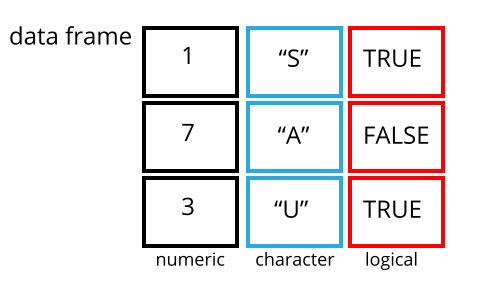
\includegraphics{./img/data-frame.png}
\caption{}
\end{figure}

We can see this when inspecting the structure of a data frame with the
function \texttt{str()}:

\begin{Shaded}
\begin{Highlighting}[]
\KeywordTok{str}\NormalTok{(surveys)}
\end{Highlighting}
\end{Shaded}

\section{\texorpdfstring{Inspecting \texttt{data.frame}
Objects}{Inspecting data.frame Objects}}\label{inspecting-data.frame-objects}

We already saw how the functions \texttt{head()} and \texttt{str()} can
be useful to check the content and the structure of a data frame. Here
is a non-exhaustive list of functions to get a sense of the
content/structure of the data. Let's try them out!

\begin{itemize}
\tightlist
\item
  Size:

  \begin{itemize}
  \tightlist
  \item
    \texttt{dim(surveys)} - returns a vector with the number of rows in
    the first element, and the number of columns as the second element
    (the \textbf{dim}ensions of the object)
  \item
    \texttt{nrow(surveys)} - returns the number of rows
  \item
    \texttt{ncol(surveys)} - returns the number of columns
  \end{itemize}
\item
  Content:

  \begin{itemize}
  \tightlist
  \item
    \texttt{head(surveys)} - shows the first 6 rows
  \item
    \texttt{tail(surveys)} - shows the last 6 rows
  \end{itemize}
\item
  Names:

  \begin{itemize}
  \tightlist
  \item
    \texttt{names(surveys)} - returns the column names (synonym of
    \texttt{colnames()} for \texttt{data.frame} objects)
  \item
    \texttt{rownames(surveys)} - returns the row names
  \end{itemize}
\item
  Summary:

  \begin{itemize}
  \tightlist
  \item
    \texttt{str(surveys)} - structure of the object and information
    about the class, length and content of each column
  \item
    \texttt{summary(surveys)} - summary statistics for each column
  \end{itemize}
\end{itemize}

Note: most of these functions are ``generic'', they can be used on other
types of objects besides \texttt{data.frame}.

\begin{quote}
\subsection{Challenge}\label{challenge-3}

Based on the output of \texttt{str(surveys)}, can you answer the
following questions?

\begin{itemize}
\tightlist
\item
  What is the class of the object \texttt{surveys}?
\item
  How many rows and how many columns are in this object?
\item
  How many species have been recorded during these surveys?
\end{itemize}

Answer

\begin{Shaded}
\begin{Highlighting}[]
\KeywordTok{str}\NormalTok{(surveys)}
\end{Highlighting}
\end{Shaded}

\begin{verbatim}
#> Classes 'tbl_df', 'tbl' and 'data.frame':  34786 obs. of  13 variables:
#>  $ record_id      : int  1 72 224 266 349 363 435 506 588 661 ...
#>  $ month          : int  7 8 9 10 11 11 12 1 2 3 ...
#>  $ day            : int  16 19 13 16 12 12 10 8 18 11 ...
#>  $ year           : int  1977 1977 1977 1977 1977 1977 1977 1978 1978 1978 ...
#>  $ plot_id        : int  2 2 2 2 2 2 2 2 2 2 ...
#>  $ species_id     : chr  "NL" "NL" "NL" "NL" ...
#>  $ sex            : chr  "M" "M" NA NA ...
#>  $ hindfoot_length: int  32 31 NA NA NA NA NA NA NA NA ...
#>  $ weight         : int  NA NA NA NA NA NA NA NA 218 NA ...
#>  $ genus          : chr  "Neotoma" "Neotoma" "Neotoma" "Neotoma" ...
#>  $ species        : chr  "albigula" "albigula" "albigula" "albigula" ...
#>  $ taxa           : chr  "Rodent" "Rodent" "Rodent" "Rodent" ...
#>  $ plot_type      : chr  "Control" "Control" "Control" "Control" ...
#>  - attr(*, "spec")=List of 2
#>   ..$ cols   :List of 13
#>   .. ..$ record_id      : list()
#>   .. .. ..- attr(*, "class")= chr  "collector_integer" "collector"
#>   .. ..$ month          : list()
#>   .. .. ..- attr(*, "class")= chr  "collector_integer" "collector"
#>   .. ..$ day            : list()
#>   .. .. ..- attr(*, "class")= chr  "collector_integer" "collector"
#>   .. ..$ year           : list()
#>   .. .. ..- attr(*, "class")= chr  "collector_integer" "collector"
#>   .. ..$ plot_id        : list()
#>   .. .. ..- attr(*, "class")= chr  "collector_integer" "collector"
#>   .. ..$ species_id     : list()
#>   .. .. ..- attr(*, "class")= chr  "collector_character" "collector"
#>   .. ..$ sex            : list()
#>   .. .. ..- attr(*, "class")= chr  "collector_character" "collector"
#>   .. ..$ hindfoot_length: list()
#>   .. .. ..- attr(*, "class")= chr  "collector_integer" "collector"
#>   .. ..$ weight         : list()
#>   .. .. ..- attr(*, "class")= chr  "collector_integer" "collector"
#>   .. ..$ genus          : list()
#>   .. .. ..- attr(*, "class")= chr  "collector_character" "collector"
#>   .. ..$ species        : list()
#>   .. .. ..- attr(*, "class")= chr  "collector_character" "collector"
#>   .. ..$ taxa           : list()
#>   .. .. ..- attr(*, "class")= chr  "collector_character" "collector"
#>   .. ..$ plot_type      : list()
#>   .. .. ..- attr(*, "class")= chr  "collector_character" "collector"
#>   ..$ default: list()
#>   .. ..- attr(*, "class")= chr  "collector_guess" "collector"
#>   ..- attr(*, "class")= chr "col_spec"
\end{verbatim}

\begin{Shaded}
\begin{Highlighting}[]
\NormalTok{## * class: data frame}
\NormalTok{## * how many rows: 34786,  how many columns: 13}
\NormalTok{## * how many species: 48}
\end{Highlighting}
\end{Shaded}
\end{quote}

\section{Indexing and subsetting data
frames}\label{indexing-and-subsetting-data-frames}

Our survey data frame has rows and columns (it has 2 dimensions), if we
want to extract some specific data from it, we need to specify the
``coordinates'' we want from it. Row numbers come first, followed by
column numbers. However, note that different ways of specifying these
coordinates lead to results with different classes.

\begin{Shaded}
\begin{Highlighting}[]
\CommentTok{# first element in the first column of the data frame (as a vector)}
\NormalTok{surveys[}\DecValTok{1}\NormalTok{, }\DecValTok{1}\NormalTok{]   }
\CommentTok{# first element in the 6th column (as a vector)}
\NormalTok{surveys[}\DecValTok{1}\NormalTok{, }\DecValTok{6}\NormalTok{]   }
\CommentTok{# first column of the data frame (as a vector)}
\NormalTok{surveys[, }\DecValTok{1}\NormalTok{]    }
\CommentTok{# first column of the data frame (as a data.frame)}
\NormalTok{surveys[}\DecValTok{1}\NormalTok{]      }
\CommentTok{# first three elements in the 7th column (as a vector)}
\NormalTok{surveys[}\DecValTok{1}\OperatorTok{:}\DecValTok{3}\NormalTok{, }\DecValTok{7}\NormalTok{] }
\CommentTok{# the 3rd row of the data frame (as a data.frame)}
\NormalTok{surveys[}\DecValTok{3}\NormalTok{, ]    }
\CommentTok{# equivalent to head_surveys <- head(surveys)}
\NormalTok{head_surveys <-}\StringTok{ }\NormalTok{surveys[}\DecValTok{1}\OperatorTok{:}\DecValTok{6}\NormalTok{, ] }
\end{Highlighting}
\end{Shaded}

\texttt{:} is a special function that creates numeric vectors of
integers in increasing or decreasing order, test \texttt{1:10} and
\texttt{10:1} for instance.

You can also exclude certain indices of a data frame using the
``\texttt{-}'' sign:

\begin{Shaded}
\begin{Highlighting}[]
\NormalTok{surveys[, }\OperatorTok{-}\DecValTok{1}\NormalTok{]          }\CommentTok{# The whole data frame, except the first column}
\NormalTok{surveys[}\OperatorTok{-}\KeywordTok{c}\NormalTok{(}\DecValTok{7}\OperatorTok{:}\DecValTok{34786}\NormalTok{), ] }\CommentTok{# Equivalent to head(surveys)}
\end{Highlighting}
\end{Shaded}

Data frames can be subset by calling indices (as shown previously), but
also by calling their column names directly:

\begin{Shaded}
\begin{Highlighting}[]
\NormalTok{surveys[}\StringTok{"species_id"}\NormalTok{]       }\CommentTok{# Result is a data.frame}
\NormalTok{surveys[, }\StringTok{"species_id"}\NormalTok{]     }\CommentTok{# Result is a vector}
\NormalTok{surveys[[}\StringTok{"species_id"}\NormalTok{]]     }\CommentTok{# Result is a vector}
\NormalTok{surveys}\OperatorTok{$}\NormalTok{species_id          }\CommentTok{# Result is a vector}
\end{Highlighting}
\end{Shaded}

In RStudio, you can use the autocompletion feature to get the full and
correct names of the columns.

\section{Formatting Dates}\label{formatting-dates}

This next section is taken from Chapter 16 of Hadley Wickham and Garrett
Grolemund's book \href{https://r4ds.had.co.nz/dates-and-times.html}{R
for Data Science} which is licensed under the
\href{https://creativecommons.org/licenses/by-nc-nd/3.0/us/}{Creative
Commons Attribution-NonCommercial-NoDerivs 3.0} license.

\subsection{Introduction}\label{introduction-1}

This chapter will show you how to work with dates and times in R. At
first glance, dates and times seem simple. You use them all the time in
your regular life, and they don't seem to cause much confusion. However,
the more you learn about dates and times, the more complicated they seem
to get. To warm up, try these three seemingly simple questions:

Does every year have 365 days? Does every day have 24 hours? Does every
minute have 60 seconds? I'm sure you know that not every year has 365
days, but do you know the full rule for determining if a year is a leap
year? (It has three parts.) You might have remembered that many parts of
the world use daylight savings time (DST), so that some days have 23
hours, and others have 25. You might not have known that some minutes
have 61 seconds because every now and then leap seconds are added
because the Earth's rotation is gradually slowing down.

Dates and times are hard because they have to reconcile two physical
phenomena (the rotation of the Earth and its orbit around the sun) with
a whole raft of geopolitical phenomena including months, time zones, and
DST. This chapter won't teach you every last detail about dates and
times, but it will give you a solid grounding of practical skills that
will help you with common data analysis challenges.

\subsection{Prerequisites}\label{prerequisites}

This chapter will focus on the \textbf{lubridate} package, which makes
it easier to work with dates and times in R. lubridate is not part of
core tidyverse because you only need it when you're working with
dates/times. We will also need nycflights13 for practice data.

\begin{Shaded}
\begin{Highlighting}[]
\KeywordTok{library}\NormalTok{(tidyverse)}
\KeywordTok{library}\NormalTok{(lubridate)}
\CommentTok{#install.packages('nycflights13')}
\KeywordTok{library}\NormalTok{(nycflights13)}
\end{Highlighting}
\end{Shaded}

\section{Creating date/times}\label{creating-datetimes}

There are three types of date/time data that refer to an instant in
time:

\begin{itemize}
\item
  A \textbf{date}. Tibbles print this as
  \texttt{\textless{}date\textgreater{}}.
\item
  A \textbf{time} within a day. Tibbles print this as
  \texttt{\textless{}time\textgreater{}}.
\item
  A \textbf{date-time} is a date plus a time: it uniquely identifies an
  instant in time (typically to the nearest second). Tibbles print this
  as \texttt{\textless{}dttm\textgreater{}}. Elsewhere in R these are
  called POSIXct, but I don't think that's a very useful name.
\end{itemize}

In this chapter we are only going to focus on dates and date-times as R
doesn't have a native class for storing times. If you need one, you can
use the \textbf{hms} package.

You should always use the simplest possible data type that works for
your needs. That means if you can use a date instead of a date-time, you
should. Date-times are substantially more complicated because of the
need to handle time zones, which we'll come back to at the end of the
chapter.

To get the current date or date-time you can use \texttt{today()} or
\texttt{now()}:

\begin{Shaded}
\begin{Highlighting}[]
\KeywordTok{today}\NormalTok{()}
\KeywordTok{now}\NormalTok{()}
\end{Highlighting}
\end{Shaded}

Otherwise, there are three ways you're likely to create a date/time:

\begin{itemize}
\tightlist
\item
  From a string.
\item
  From individual date-time components.
\item
  From an existing date/time object.
\end{itemize}

They work as follows.

\subsection{From strings}\label{from-strings}

Date/time data often comes as strings. You've seen one approach to
parsing strings into date-times in
\protect\hyperlink{readr-datetimes}{date-times}. Another approach is to
use the helpers provided by lubridate. They automatically work out the
format once you specify the order of the component. To use them,
identify the order in which year, month, and day appear in your dates,
then arrange ``y'', ``m'', and ``d'' in the same order. That gives you
the name of the lubridate function that will parse your date. For
example:

\begin{Shaded}
\begin{Highlighting}[]
\KeywordTok{ymd}\NormalTok{(}\StringTok{"2017-01-31"}\NormalTok{)}
\KeywordTok{mdy}\NormalTok{(}\StringTok{"January 31st, 2017"}\NormalTok{)}
\KeywordTok{dmy}\NormalTok{(}\StringTok{"31-Jan-2017"}\NormalTok{)}
\end{Highlighting}
\end{Shaded}

These functions also take unquoted numbers. This is the most concise way
to create a single date/time object, as you might need when filtering
date/time data. \texttt{ymd()} is short and unambiguous:

\begin{Shaded}
\begin{Highlighting}[]
\KeywordTok{ymd}\NormalTok{(}\DecValTok{20170131}\NormalTok{)}
\end{Highlighting}
\end{Shaded}

\texttt{ymd()} and friends create dates. To create a date-time, add an
underscore and one or more of ``h'', ``m'', and ``s'' to the name of the
parsing function:

\begin{Shaded}
\begin{Highlighting}[]
\KeywordTok{ymd_hms}\NormalTok{(}\StringTok{"2017-01-31 20:11:59"}\NormalTok{)}
\KeywordTok{mdy_hm}\NormalTok{(}\StringTok{"01/31/2017 08:01"}\NormalTok{)}
\end{Highlighting}
\end{Shaded}

You can also force the creation of a date-time from a date by supplying
a timezone:

\begin{Shaded}
\begin{Highlighting}[]
\KeywordTok{ymd}\NormalTok{(}\DecValTok{20170131}\NormalTok{, }\DataTypeTok{tz =} \StringTok{"UTC"}\NormalTok{)}
\end{Highlighting}
\end{Shaded}

\subsection{From other types}\label{from-other-types}

You may want to switch between a date-time and a date. That's the job of
\texttt{as\_datetime()} and \texttt{as\_date()}:

\begin{Shaded}
\begin{Highlighting}[]
\KeywordTok{as_datetime}\NormalTok{(}\KeywordTok{today}\NormalTok{())}
\KeywordTok{as_date}\NormalTok{(}\KeywordTok{now}\NormalTok{())}
\end{Highlighting}
\end{Shaded}

Sometimes you'll get date/times as numeric offsets from the ``Unix
Epoch'', 1970-01-01. If the offset is in seconds, use
\texttt{as\_datetime()}; if it's in days, use \texttt{as\_date()}.

\begin{Shaded}
\begin{Highlighting}[]
\KeywordTok{as_datetime}\NormalTok{(}\DecValTok{60} \OperatorTok{*}\StringTok{ }\DecValTok{60} \OperatorTok{*}\StringTok{ }\DecValTok{10}\NormalTok{)}
\KeywordTok{as_date}\NormalTok{(}\DecValTok{365} \OperatorTok{*}\StringTok{ }\DecValTok{10} \OperatorTok{+}\StringTok{ }\DecValTok{2}\NormalTok{)}
\end{Highlighting}
\end{Shaded}

\subsection{Exercises}\label{exercises}

\begin{enumerate}
\def\labelenumi{\arabic{enumi}.}
\item
  What happens if you parse a string that contains invalid dates?

\begin{Shaded}
\begin{Highlighting}[]
\KeywordTok{ymd}\NormalTok{(}\KeywordTok{c}\NormalTok{(}\StringTok{"2010-10-10"}\NormalTok{, }\StringTok{"bananas"}\NormalTok{))}
\end{Highlighting}
\end{Shaded}
\item
  What does the \texttt{tzone} argument to \texttt{today()} do? Why is
  it important?
\item
  Use the appropriate lubridate function to parse each of the following
  dates:

\begin{Shaded}
\begin{Highlighting}[]
\NormalTok{d1 <-}\StringTok{ "January 1, 2010"}
\NormalTok{d2 <-}\StringTok{ "2015-Mar-07"}
\NormalTok{d3 <-}\StringTok{ "06-Jun-2017"}
\NormalTok{d4 <-}\StringTok{ }\KeywordTok{c}\NormalTok{(}\StringTok{"August 19 (2015)"}\NormalTok{, }\StringTok{"July 1 (2015)"}\NormalTok{)}
\NormalTok{d5 <-}\StringTok{ "12/30/14"} \CommentTok{# Dec 30, 2014}
\end{Highlighting}
\end{Shaded}
\end{enumerate}

\section{Date-time components}\label{date-time-components}

Now that you know how to get date-time data into R's date-time data
structures, let's explore what you can do with them. This section will
focus on the accessor functions that let you get and set individual
components. The next section will look at how arithmetic works with
date-times.

\subsection{Getting components}\label{getting-components}

You can pull out individual parts of the date with the accessor
functions \texttt{year()}, \texttt{month()}, \texttt{mday()} (day of the
month), \texttt{yday()} (day of the year), \texttt{wday()} (day of the
week), \texttt{hour()}, \texttt{minute()}, and \texttt{second()}.

\begin{Shaded}
\begin{Highlighting}[]
\NormalTok{datetime <-}\StringTok{ }\KeywordTok{ymd_hms}\NormalTok{(}\StringTok{"2016-07-08 12:34:56"}\NormalTok{)}
\KeywordTok{year}\NormalTok{(datetime)}
\KeywordTok{month}\NormalTok{(datetime)}
\KeywordTok{mday}\NormalTok{(datetime)}
\KeywordTok{yday}\NormalTok{(datetime)}
\KeywordTok{wday}\NormalTok{(datetime)}
\end{Highlighting}
\end{Shaded}

For \texttt{month()} and \texttt{wday()} you can set
\texttt{label\ =\ TRUE} to return the abbreviated name of the month or
day of the week. Set \texttt{abbr\ =\ FALSE} to return the full name.

\begin{Shaded}
\begin{Highlighting}[]
\KeywordTok{month}\NormalTok{(datetime, }\DataTypeTok{label =} \OtherTok{TRUE}\NormalTok{)}
\KeywordTok{wday}\NormalTok{(datetime, }\DataTypeTok{label =} \OtherTok{TRUE}\NormalTok{, }\DataTypeTok{abbr =} \OtherTok{FALSE}\NormalTok{)}
\end{Highlighting}
\end{Shaded}

\section{Time spans}\label{time-spans}

Next you'll learn about how arithmetic with dates works, including
subtraction, addition, and division. Along the way, you'll learn about
three important classes that represent time spans:

\begin{itemize}
\tightlist
\item
  \textbf{durations}, which represent an exact number of seconds.
\item
  \textbf{periods}, which represent human units like weeks and months.
\item
  \textbf{intervals}, which represent a starting and ending point.
\end{itemize}

\subsection{Durations}\label{durations}

In R, when you subtract two dates, you get a difftime object:

\begin{Shaded}
\begin{Highlighting}[]
\CommentTok{# How old is Hadley?}
\NormalTok{h_age <-}\StringTok{ }\KeywordTok{today}\NormalTok{() }\OperatorTok{-}\StringTok{ }\KeywordTok{ymd}\NormalTok{(}\DecValTok{19791014}\NormalTok{)}
\NormalTok{h_age}
\end{Highlighting}
\end{Shaded}

For more see \href{https://r4ds.had.co.nz/dates-and-times.html}{R for
Data Science}.

\chapter{Manipulating and analyzing data with
dplyr}\label{manipulating-and-analyzing-data-with-dplyr}

\begin{center}\rule{0.5\linewidth}{\linethickness}\end{center}

\begin{quote}
\subsection{Learning Objectives}\label{learning-objectives-3}

\begin{itemize}
\tightlist
\item
  Describe the purpose of the \textbf{\texttt{dplyr}} and
  \textbf{\texttt{tidyr}} packages.
\item
  Select certain columns in a data frame with the
  \textbf{\texttt{dplyr}} function \texttt{select}.
\item
  Select certain rows in a data frame according to filtering conditions
  with the \textbf{\texttt{dplyr}} function \texttt{filter} .
\item
  Link the output of one \textbf{\texttt{dplyr}} function to the input
  of another function with the `pipe' operator
  \texttt{\%\textgreater{}\%}.
\item
  Add new columns to a data frame that are functions of existing columns
  with \texttt{mutate}.
\item
  Use the split-apply-combine concept for data analysis.
\item
  Use \texttt{summarize}, \texttt{group\_by}, and \texttt{count} to
  split a data frame into groups of observations, apply a summary
  statistics for each group, and then combine the results.
\item
  Describe the concept of a wide and a long table format and for which
  purpose those formats are useful.
\item
  Describe what key-value pairs are.
\item
  Reshape a data frame from long to wide format and back with the
  \texttt{spread} and \texttt{gather} commands from the
  \textbf{\texttt{tidyr}} package.
\item
  Export a data frame to a .csv file. Work with Factors in R
\end{itemize}
\end{quote}

\begin{center}\rule{0.5\linewidth}{\linethickness}\end{center}

\section{\texorpdfstring{Data Manipulation using \textbf{\texttt{dplyr}}
and
\textbf{\texttt{tidyr}}}{Data Manipulation using dplyr and tidyr}}\label{data-manipulation-using-dplyr-and-tidyr}

Bracket subsetting is handy, but it can be cumbersome and difficult to
read, especially for complicated operations. Enter
\textbf{\texttt{dplyr}}. \textbf{\texttt{dplyr}} is a package for making
tabular data manipulation easier. It pairs nicely with
\textbf{\texttt{tidyr}} which enables you to swiftly convert between
different data formats for plotting and analysis.

Packages in R are basically sets of additional functions that let you do
more stuff. The functions we've been using so far, like \texttt{str()}
or \texttt{data.frame()}, come built into R; packages give you access to
more of them. Before you use a package for the first time you need to
install it on your machine, and then you should import it in every
subsequent R session when you need it. You should already have installed
the \textbf{\texttt{tidyverse}} package. This is an ``umbrella-package''
that installs several packages useful for data analysis which work
together well such as \textbf{\texttt{tidyr}}, \textbf{\texttt{dplyr}},
\textbf{\texttt{ggplot2}}, \textbf{\texttt{tibble}}, etc.

To load the package type:

\begin{Shaded}
\begin{Highlighting}[]
\NormalTok{## load the tidyverse packages, incl. dplyr}
\KeywordTok{library}\NormalTok{(}\StringTok{"tidyverse"}\NormalTok{)}
\end{Highlighting}
\end{Shaded}

\section{\texorpdfstring{What are \textbf{\texttt{dplyr}} and
\textbf{\texttt{tidyr}}?}{What are dplyr and tidyr?}}\label{what-are-dplyr-and-tidyr}

The package \textbf{\texttt{dplyr}} provides easy tools for the most
common data manipulation tasks. It is built to work directly with data
frames, with many common tasks optimized by being written in a compiled
language (C++). An additional feature is the ability to work directly
with data stored in an external database. The benefits of doing this are
that the data can be managed natively in a relational database, queries
can be conducted on that database, and only the results of the query are
returned.

This addresses a common problem with R in that all operations are
conducted in-memory and thus the amount of data you can work with is
limited by available memory. The database connections essentially remove
that limitation in that you can connect to a database of many hundreds
of GB, conduct queries on it directly, and pull back into R only what
you need for analysis.

The package \textbf{\texttt{tidyr}} addresses the common problem of
wanting to reshape your data for plotting and use by different R
functions. Sometimes we want data sets where we have one row per
measurement. Sometimes we want a data frame where each measurement type
has its own column, and rows are instead more aggregated groups - like
plots or aquaria. Moving back and forth between these formats is
nontrivial, and \textbf{\texttt{tidyr}} gives you tools for this and
more sophisticated data manipulation.

To learn more about \textbf{\texttt{dplyr}} and \textbf{\texttt{tidyr}}
after the workshop, you may want to check out this
\href{https://github.com/rstudio/cheatsheets/raw/master/data-transformation.pdf}{handy
data transformation with \textbf{\texttt{dplyr}} cheatsheet} and this
\href{https://github.com/rstudio/cheatsheets/raw/master/data-import.pdf}{one
about \textbf{\texttt{tidyr}}}.

\begin{Shaded}
\begin{Highlighting}[]
\NormalTok{surveys <-}\StringTok{ }\KeywordTok{read_csv}\NormalTok{(}\StringTok{"data/portal_data_joined.csv"}\NormalTok{)}
\end{Highlighting}
\end{Shaded}

\begin{verbatim}
#> Parsed with column specification:
#> cols(
#>   record_id = col_integer(),
#>   month = col_integer(),
#>   day = col_integer(),
#>   year = col_integer(),
#>   plot_id = col_integer(),
#>   species_id = col_character(),
#>   sex = col_character(),
#>   hindfoot_length = col_integer(),
#>   weight = col_integer(),
#>   genus = col_character(),
#>   species = col_character(),
#>   taxa = col_character(),
#>   plot_type = col_character()
#> )
\end{verbatim}

\begin{Shaded}
\begin{Highlighting}[]
\NormalTok{## inspect the data}
\KeywordTok{str}\NormalTok{(surveys)}

\NormalTok{## preview the data}
\CommentTok{# View(surveys)}
\end{Highlighting}
\end{Shaded}

We're going to learn some of the most common \textbf{\texttt{dplyr}}
functions:

\begin{itemize}
\tightlist
\item
  \texttt{select()}: subset columns
\item
  \texttt{filter()}: subset rows on conditions
\item
  \texttt{mutate()}: create new columns by using information from other
  columns
\item
  \texttt{group\_by()} and \texttt{summarize()}: create summary
  statisitcs on grouped data
\item
  \texttt{arrange()}: sort results
\item
  \texttt{count()}: count discrete values
\end{itemize}

\section{Selecting columns and filtering
rows}\label{selecting-columns-and-filtering-rows}

To select columns of a data frame, use \texttt{select()}. The first
argument to this function is the data frame (\texttt{surveys}), and the
subsequent arguments are the columns to keep.

\begin{Shaded}
\begin{Highlighting}[]
\KeywordTok{select}\NormalTok{(surveys, plot_id, species_id, weight)}
\end{Highlighting}
\end{Shaded}

To select all columns \emph{except} certain ones, put a ``-'' in front
of the variable to exclude it.

\begin{Shaded}
\begin{Highlighting}[]
\KeywordTok{select}\NormalTok{(surveys, }\OperatorTok{-}\NormalTok{record_id, }\OperatorTok{-}\NormalTok{species_id)}
\end{Highlighting}
\end{Shaded}

This will select all the variables in \texttt{surveys} except
\texttt{record\_id} and \texttt{species\_id}.

To choose rows based on a specific criteria, use \texttt{filter()}:

\begin{Shaded}
\begin{Highlighting}[]
\KeywordTok{filter}\NormalTok{(surveys, year }\OperatorTok{==}\StringTok{ }\DecValTok{1995}\NormalTok{)}
\end{Highlighting}
\end{Shaded}

\section{Pipes}\label{pipes}

What if you want to select and filter at the same time? There are three
ways to do this: use intermediate steps, nested functions, or pipes.

With intermediate steps, you create a temporary data frame and use that
as input to the next function, like this:

\begin{Shaded}
\begin{Highlighting}[]
\NormalTok{surveys2 <-}\StringTok{ }\KeywordTok{filter}\NormalTok{(surveys, weight }\OperatorTok{<}\StringTok{ }\DecValTok{5}\NormalTok{)}
\NormalTok{surveys_sml <-}\StringTok{ }\KeywordTok{select}\NormalTok{(surveys2, species_id, sex, weight)}
\end{Highlighting}
\end{Shaded}

This is readable, but can clutter up your workspace with lots of objects
that you have to name individually. With multiple steps, that can be
hard to keep track of.

You can also nest functions (i.e.~one function inside of another), like
this:

\begin{Shaded}
\begin{Highlighting}[]
\NormalTok{surveys_sml <-}\StringTok{ }\KeywordTok{select}\NormalTok{(}\KeywordTok{filter}\NormalTok{(surveys, weight }\OperatorTok{<}\StringTok{ }\DecValTok{5}\NormalTok{), species_id, sex, weight)}
\end{Highlighting}
\end{Shaded}

This is handy, but can be difficult to read if too many functions are
nested, as R evaluates the expression from the inside out (in this case,
filtering, then selecting).

The last option, \emph{pipes}, are a recent addition to R. Pipes let you
take the output of one function and send it directly to the next, which
is useful when you need to do many things to the same dataset. Pipes in
R look like \texttt{\%\textgreater{}\%} and are made available via the
\textbf{\texttt{magrittr}} package, installed automatically with
\textbf{\texttt{dplyr}}. If you use RStudio, you can type the pipe with
Ctrl + Shift + M if you have a PC or Cmd + Shift + M if you have a Mac.

\begin{Shaded}
\begin{Highlighting}[]
\NormalTok{surveys }\OperatorTok
\StringTok{  }\KeywordTok{filter}\NormalTok{(weight }\OperatorTok{<}\StringTok{ }\DecValTok{5}\NormalTok{) }\OperatorTok
\StringTok{  }\KeywordTok{select}\NormalTok{(species_id, sex, weight)}
\end{Highlighting}
\end{Shaded}

In the above code, we use the pipe to send the \texttt{surveys} dataset
first through \texttt{filter()} to keep rows where \texttt{weight} is
less than 5, then through \texttt{select()} to keep only the
\texttt{species\_id}, \texttt{sex}, and \texttt{weight} columns. Since
\texttt{\%\textgreater{}\%} takes the object on its left and passes it
as the first argument to the function on its right, we don't need to
explicitly include the data frame as an argument to the
\texttt{filter()} and \texttt{select()} functions any more.

Some may find it helpful to read the pipe like the word ``then''. For
instance, in the above example, we took the data frame \texttt{surveys},
\emph{then} we \texttt{filter}ed for rows with
\texttt{weight\ \textless{}\ 5}, \emph{then} we \texttt{select}ed
columns \texttt{species\_id}, \texttt{sex}, and \texttt{weight}. The
\textbf{\texttt{dplyr}} functions by themselves are somewhat simple, but
by combining them into linear workflows with the pipe, we can accomplish
more complex manipulations of data frames.

If we want to create a new object with this smaller version of the data,
we can assign it a new name:

\begin{Shaded}
\begin{Highlighting}[]
\NormalTok{surveys_sml <-}\StringTok{ }\NormalTok{surveys }\OperatorTok
\StringTok{  }\KeywordTok{filter}\NormalTok{(weight }\OperatorTok{<}\StringTok{ }\DecValTok{5}\NormalTok{) }\OperatorTok
\StringTok{  }\KeywordTok{select}\NormalTok{(species_id, sex, weight)}

\NormalTok{surveys_sml}
\end{Highlighting}
\end{Shaded}

Note that the final data frame is the leftmost part of this expression.

\begin{quote}
\subsection{Challenge}\label{challenge-4}

Using pipes, subset the \texttt{surveys} data to include animals
collected before 1995 and retain only the columns \texttt{year},
\texttt{sex}, and \texttt{weight}.

Answer

\begin{Shaded}
\begin{Highlighting}[]
\NormalTok{surveys }\OperatorTok
\StringTok{    }\KeywordTok{filter}\NormalTok{(year }\OperatorTok{<}\StringTok{ }\DecValTok{1995}\NormalTok{) }\OperatorTok
\StringTok{    }\KeywordTok{select}\NormalTok{(year, sex, weight)}
\end{Highlighting}
\end{Shaded}
\end{quote}

\subsection{Mutate}\label{mutate}

Frequently you'll want to create new columns based on the values in
existing columns, for example to do unit conversions, or to find the
ratio of values in two columns. For this we'll use \texttt{mutate()}.

To create a new column of weight in kg:

\begin{Shaded}
\begin{Highlighting}[]
\NormalTok{surveys }\OperatorTok
\StringTok{  }\KeywordTok{mutate}\NormalTok{(}\DataTypeTok{weight_kg =}\NormalTok{ weight }\OperatorTok{/}\StringTok{ }\DecValTok{1000}\NormalTok{)}
\end{Highlighting}
\end{Shaded}

You can also create a second new column based on the first new column
within the same call of \texttt{mutate()}:

\begin{Shaded}
\begin{Highlighting}[]
\NormalTok{surveys }\OperatorTok
\StringTok{  }\KeywordTok{mutate}\NormalTok{(}\DataTypeTok{weight_kg =}\NormalTok{ weight }\OperatorTok{/}\StringTok{ }\DecValTok{1000}\NormalTok{,}
         \DataTypeTok{weight_kg2 =}\NormalTok{ weight_kg }\OperatorTok{*}\StringTok{ }\DecValTok{2}\NormalTok{)}
\end{Highlighting}
\end{Shaded}

If this runs off your screen and you just want to see the first few
rows, you can use a pipe to view the \texttt{head()} of the data. (Pipes
work with non-\textbf{\texttt{dplyr}} functions, too, as long as the
\textbf{\texttt{dplyr}} or \texttt{magrittr} package is loaded).

\begin{Shaded}
\begin{Highlighting}[]
\NormalTok{surveys }\OperatorTok
\StringTok{  }\KeywordTok{mutate}\NormalTok{(}\DataTypeTok{weight_kg =}\NormalTok{ weight }\OperatorTok{/}\StringTok{ }\DecValTok{1000}\NormalTok{) }\OperatorTok
\StringTok{  }\KeywordTok{head}\NormalTok{()}
\end{Highlighting}
\end{Shaded}

The first few rows of the output are full of \texttt{NA}s, so if we
wanted to remove those we could insert a \texttt{filter()} in the chain:

\begin{Shaded}
\begin{Highlighting}[]
\NormalTok{surveys }\OperatorTok
\StringTok{  }\KeywordTok{filter}\NormalTok{(}\OperatorTok{!}\KeywordTok{is.na}\NormalTok{(weight)) }\OperatorTok
\StringTok{  }\KeywordTok{mutate}\NormalTok{(}\DataTypeTok{weight_kg =}\NormalTok{ weight }\OperatorTok{/}\StringTok{ }\DecValTok{1000}\NormalTok{) }\OperatorTok
\StringTok{  }\KeywordTok{head}\NormalTok{()}
\end{Highlighting}
\end{Shaded}

\texttt{is.na()} is a function that determines whether something is an
\texttt{NA}. The \texttt{!} symbol negates the result, so we're asking
for every row where weight \emph{is not} an \texttt{NA}.

\begin{quote}
\subsection{Challenge}\label{challenge-5}

Create a new data frame from the \texttt{surveys} data that meets the
following criteria: contains only the \texttt{species\_id} column and a
new column called \texttt{hindfoot\_half} containing values that are
half the \texttt{hindfoot\_length} values. In this
\texttt{hindfoot\_half} column, there are no \texttt{NA}s and all values
are less than 30.

\textbf{Hint}: think about how the commands should be ordered to produce
this data frame!

Answer

\begin{Shaded}
\begin{Highlighting}[]
\NormalTok{surveys_hindfoot_half <-}\StringTok{ }\NormalTok{surveys }\OperatorTok
\StringTok{    }\KeywordTok{filter}\NormalTok{(}\OperatorTok{!}\KeywordTok{is.na}\NormalTok{(hindfoot_length)) }\OperatorTok
\StringTok{    }\KeywordTok{mutate}\NormalTok{(}\DataTypeTok{hindfoot_half =}\NormalTok{ hindfoot_length }\OperatorTok{/}\StringTok{ }\DecValTok{2}\NormalTok{) }\OperatorTok
\StringTok{    }\KeywordTok{filter}\NormalTok{(hindfoot_half }\OperatorTok{<}\StringTok{ }\DecValTok{30}\NormalTok{) }\OperatorTok
\StringTok{    }\KeywordTok{select}\NormalTok{(species_id, hindfoot_half)}
\end{Highlighting}
\end{Shaded}
\end{quote}

\subsection{\texorpdfstring{The \texttt{summarize()}
function}{The summarize() function}}\label{the-summarize-function}

\texttt{group\_by()} is often used together with \texttt{summarize()},
which collapses each group into a single-row summary of that group.
\texttt{group\_by()} takes as arguments the column names that contain
the \textbf{categorical} variables for which you want to calculate the
summary statistics. So to compute the mean \texttt{weight} by sex:

\begin{Shaded}
\begin{Highlighting}[]
\NormalTok{surveys }\OperatorTok
\StringTok{  }\KeywordTok{group_by}\NormalTok{(sex) }\OperatorTok
\StringTok{  }\KeywordTok{summarize}\NormalTok{(}\DataTypeTok{mean_weight =} \KeywordTok{mean}\NormalTok{(weight, }\DataTypeTok{na.rm =} \OtherTok{TRUE}\NormalTok{))}
\end{Highlighting}
\end{Shaded}

You may also have noticed that the output from these calls doesn't run
off the screen anymore. It's one of the advantages of \texttt{tbl\_df}
over data frame.

You can also group by multiple columns:

\begin{Shaded}
\begin{Highlighting}[]
\NormalTok{surveys }\OperatorTok
\StringTok{  }\KeywordTok{group_by}\NormalTok{(sex, species_id) }\OperatorTok
\StringTok{  }\KeywordTok{summarize}\NormalTok{(}\DataTypeTok{mean_weight =} \KeywordTok{mean}\NormalTok{(weight, }\DataTypeTok{na.rm =} \OtherTok{TRUE}\NormalTok{))}
\end{Highlighting}
\end{Shaded}

When grouping both by \texttt{sex} and \texttt{species\_id}, the last
few rows are for animals that escaped before their sex and body weights
could be determined. You may notice that the last column does not
contain \texttt{NA} but \texttt{NaN} (which refers to ``Not a Number'').
To avoid this, we can remove the missing values for weight before we
attempt to calculate the summary statistics on weight. Because the
missing values are removed first, we can omit \texttt{na.rm\ =\ TRUE}
when computing the mean:

\begin{Shaded}
\begin{Highlighting}[]
\NormalTok{surveys }\OperatorTok
\StringTok{  }\KeywordTok{filter}\NormalTok{(}\OperatorTok{!}\KeywordTok{is.na}\NormalTok{(weight)) }\OperatorTok
\StringTok{  }\KeywordTok{group_by}\NormalTok{(sex, species_id) }\OperatorTok
\StringTok{  }\KeywordTok{summarize}\NormalTok{(}\DataTypeTok{mean_weight =} \KeywordTok{mean}\NormalTok{(weight))}
\end{Highlighting}
\end{Shaded}

Here, again, the output from these calls doesn't run off the screen
anymore. If you want to display more data, you can use the
\texttt{print()} function at the end of your chain with the argument
\texttt{n} specifying the number of rows to display:

\begin{Shaded}
\begin{Highlighting}[]
\NormalTok{surveys }\OperatorTok
\StringTok{  }\KeywordTok{filter}\NormalTok{(}\OperatorTok{!}\KeywordTok{is.na}\NormalTok{(weight)) }\OperatorTok
\StringTok{  }\KeywordTok{group_by}\NormalTok{(sex, species_id) }\OperatorTok
\StringTok{  }\KeywordTok{summarize}\NormalTok{(}\DataTypeTok{mean_weight =} \KeywordTok{mean}\NormalTok{(weight)) }\OperatorTok
\StringTok{  }\KeywordTok{print}\NormalTok{(}\DataTypeTok{n =} \DecValTok{15}\NormalTok{)}
\end{Highlighting}
\end{Shaded}

Once the data are grouped, you can also summarize multiple variables at
the same time (and not necessarily on the same variable). For instance,
we could add a column indicating the minimum weight for each species for
each sex:

\begin{Shaded}
\begin{Highlighting}[]
\NormalTok{surveys }\OperatorTok
\StringTok{  }\KeywordTok{filter}\NormalTok{(}\OperatorTok{!}\KeywordTok{is.na}\NormalTok{(weight)) }\OperatorTok
\StringTok{  }\KeywordTok{group_by}\NormalTok{(sex, species_id) }\OperatorTok
\StringTok{  }\KeywordTok{summarize}\NormalTok{(}\DataTypeTok{mean_weight =} \KeywordTok{mean}\NormalTok{(weight),}
            \DataTypeTok{min_weight =} \KeywordTok{min}\NormalTok{(weight))}
\end{Highlighting}
\end{Shaded}

It is sometimes useful to rearrange the result of a query to inspect the
values. For instance, we can sort on \texttt{min\_weight} to put the
lighter species first:

\begin{Shaded}
\begin{Highlighting}[]
\NormalTok{surveys }\OperatorTok
\StringTok{  }\KeywordTok{filter}\NormalTok{(}\OperatorTok{!}\KeywordTok{is.na}\NormalTok{(weight)) }\OperatorTok
\StringTok{  }\KeywordTok{group_by}\NormalTok{(sex, species_id) }\OperatorTok
\StringTok{  }\KeywordTok{summarize}\NormalTok{(}\DataTypeTok{mean_weight =} \KeywordTok{mean}\NormalTok{(weight),}
            \DataTypeTok{min_weight =} \KeywordTok{min}\NormalTok{(weight)) }\OperatorTok
\StringTok{  }\KeywordTok{arrange}\NormalTok{(min_weight)}
\end{Highlighting}
\end{Shaded}

To sort in descending order, we need to add the \texttt{desc()}
function. If we want to sort the results by decreasing order of mean
weight:

\begin{Shaded}
\begin{Highlighting}[]
\NormalTok{surveys }\OperatorTok
\StringTok{  }\KeywordTok{filter}\NormalTok{(}\OperatorTok{!}\KeywordTok{is.na}\NormalTok{(weight)) }\OperatorTok
\StringTok{  }\KeywordTok{group_by}\NormalTok{(sex, species_id) }\OperatorTok
\StringTok{  }\KeywordTok{summarize}\NormalTok{(}\DataTypeTok{mean_weight =} \KeywordTok{mean}\NormalTok{(weight),}
            \DataTypeTok{min_weight =} \KeywordTok{min}\NormalTok{(weight)) }\OperatorTok
\StringTok{  }\KeywordTok{arrange}\NormalTok{(}\KeywordTok{desc}\NormalTok{(mean_weight))}
\end{Highlighting}
\end{Shaded}

\subsection{Counting}\label{counting}

When working with data, we often want to know the number of observations
found for each factor or combination of factors. For this task,
\textbf{\texttt{dplyr}} provides \texttt{count()}. For example, if we
wanted to count the number of rows of data for each sex, we would do:

\begin{Shaded}
\begin{Highlighting}[]
\NormalTok{surveys }\OperatorTok
\StringTok{    }\KeywordTok{count}\NormalTok{(sex) }
\end{Highlighting}
\end{Shaded}

The \texttt{count()} function is shorthand for something we've already
seen: grouping by a variable, and summarizing it by counting the number
of observations in that group. In other words,
\texttt{surveys\ \%\textgreater{}\%\ count()} is equivalent to:

\begin{Shaded}
\begin{Highlighting}[]
\NormalTok{surveys }\OperatorTok
\StringTok{    }\KeywordTok{group_by}\NormalTok{(sex) }\OperatorTok
\StringTok{    }\KeywordTok{summarise}\NormalTok{(}\DataTypeTok{count =} \KeywordTok{n}\NormalTok{())}
\end{Highlighting}
\end{Shaded}

For convenience, \texttt{count()} provides the \texttt{sort} argument:

\begin{Shaded}
\begin{Highlighting}[]
\NormalTok{surveys }\OperatorTok
\StringTok{    }\KeywordTok{count}\NormalTok{(sex, }\DataTypeTok{sort =} \OtherTok{TRUE}\NormalTok{) }
\end{Highlighting}
\end{Shaded}

\begin{quote}
\subsection{Challenge}\label{challenge-6}

\begin{enumerate}
\def\labelenumi{\arabic{enumi}.}
\tightlist
\item
  How many animals were caught in each \texttt{plot\_type} surveyed?
\end{enumerate}

Answer

\begin{Shaded}
\begin{Highlighting}[]
\NormalTok{surveys }\OperatorTok
\StringTok{    }\KeywordTok{count}\NormalTok{(plot_type) }
\end{Highlighting}
\end{Shaded}

\begin{enumerate}
\def\labelenumi{\arabic{enumi}.}
\setcounter{enumi}{1}
\tightlist
\item
  Use \texttt{group\_by()} and \texttt{summarize()} to find the mean,
  min, and max hindfoot length for each species (using
  \texttt{species\_id}). Also add the number of observations (hint: see
  \texttt{?n}).
\end{enumerate}

Answer

\begin{Shaded}
\begin{Highlighting}[]
\NormalTok{surveys }\OperatorTok
\StringTok{    }\KeywordTok{filter}\NormalTok{(}\OperatorTok{!}\KeywordTok{is.na}\NormalTok{(hindfoot_length)) }\OperatorTok
\StringTok{    }\KeywordTok{group_by}\NormalTok{(species_id) }\OperatorTok
\StringTok{    }\KeywordTok{summarize}\NormalTok{(}
        \DataTypeTok{mean_hindfoot_length =} \KeywordTok{mean}\NormalTok{(hindfoot_length),}
        \DataTypeTok{min_hindfoot_length =} \KeywordTok{min}\NormalTok{(hindfoot_length),}
        \DataTypeTok{max_hindfoot_length =} \KeywordTok{max}\NormalTok{(hindfoot_length),}
        \DataTypeTok{n =} \KeywordTok{n}\NormalTok{()}
\NormalTok{    )}
\end{Highlighting}
\end{Shaded}

\begin{enumerate}
\def\labelenumi{\arabic{enumi}.}
\setcounter{enumi}{2}
\tightlist
\item
  What was the heaviest animal measured in each year? Return the columns
  \texttt{year}, \texttt{genus}, \texttt{species\_id}, and
  \texttt{weight}.
\end{enumerate}

Answer

\begin{Shaded}
\begin{Highlighting}[]
\NormalTok{surveys }\OperatorTok
\StringTok{    }\KeywordTok{filter}\NormalTok{(}\OperatorTok{!}\KeywordTok{is.na}\NormalTok{(weight)) }\OperatorTok
\StringTok{    }\KeywordTok{group_by}\NormalTok{(year) }\OperatorTok
\StringTok{    }\KeywordTok{filter}\NormalTok{(weight }\OperatorTok{==}\StringTok{ }\KeywordTok{max}\NormalTok{(weight)) }\OperatorTok
\StringTok{    }\KeywordTok{select}\NormalTok{(year, genus, species, weight) }\OperatorTok
\StringTok{    }\KeywordTok{arrange}\NormalTok{(year)}
\end{Highlighting}
\end{Shaded}
\end{quote}

\subsection{Reshaping with gather and
spread}\label{reshaping-with-gather-and-spread}

In the
\href{http://www.datacarpentry.org/spreadsheet-ecology-lesson/01-format-data/}{spreadsheet
lesson}, we discussed how to structure our data leading to the four
rules defining a tidy dataset:

\begin{enumerate}
\def\labelenumi{\arabic{enumi}.}
\tightlist
\item
  Each variable has its own column
\item
  Each observation has its own row
\item
  Each value must have its own cell
\item
  Each type of observational unit forms a table
\end{enumerate}

Sometimes your you want to spread the observations of on variable across
multiple columns.

\subsubsection{Spreading}\label{spreading}

\texttt{spread()} takes three principal arguments:

\begin{enumerate}
\def\labelenumi{\arabic{enumi}.}
\tightlist
\item
  the data
\item
  the \emph{key} column variable whose values will become new column
  names.\\
\item
  the \emph{value} column variable whose values will fill the new column
  variables.
\end{enumerate}

Further arguments include \texttt{fill} which, if set, fills in missing
values with the value provided.

Let's use \texttt{spread()} to transform surveys to find the mean weight
of each species in each plot over the entire survey period. We use
\texttt{filter()}, \texttt{group\_by()} and \texttt{summarise()} to
filter our observations and variables of interest, and create a new
variable for the \texttt{mean\_weight}. We use the pipe as before too.

\begin{Shaded}
\begin{Highlighting}[]
\NormalTok{surveys_gw <-}\StringTok{ }\NormalTok{surveys }\OperatorTok
\StringTok{  }\KeywordTok{filter}\NormalTok{(}\OperatorTok{!}\KeywordTok{is.na}\NormalTok{(weight)) }\OperatorTok
\StringTok{  }\KeywordTok{group_by}\NormalTok{(genus, plot_id) }\OperatorTok
\StringTok{  }\KeywordTok{summarize}\NormalTok{(}\DataTypeTok{mean_weight =} \KeywordTok{mean}\NormalTok{(weight))}

\KeywordTok{str}\NormalTok{(surveys_gw)}
\end{Highlighting}
\end{Shaded}

This yields \texttt{surveys\_gw} where the observations for each plot
are spread across multiple rows, 196 observations of 3 variables. Using
\texttt{spread()} to key on \texttt{genus} with values from
\texttt{mean\_weight} this becomes 24 observations of 11 variables, one
row for each plot. We again use pipes:

\begin{Shaded}
\begin{Highlighting}[]
\NormalTok{surveys_spread <-}\StringTok{ }\NormalTok{surveys_gw }\OperatorTok
\StringTok{  }\KeywordTok{spread}\NormalTok{(}\DataTypeTok{key =}\NormalTok{ genus, }\DataTypeTok{value =}\NormalTok{ mean_weight)}

\KeywordTok{str}\NormalTok{(surveys_spread)}
\end{Highlighting}
\end{Shaded}

\begin{figure}
\centering
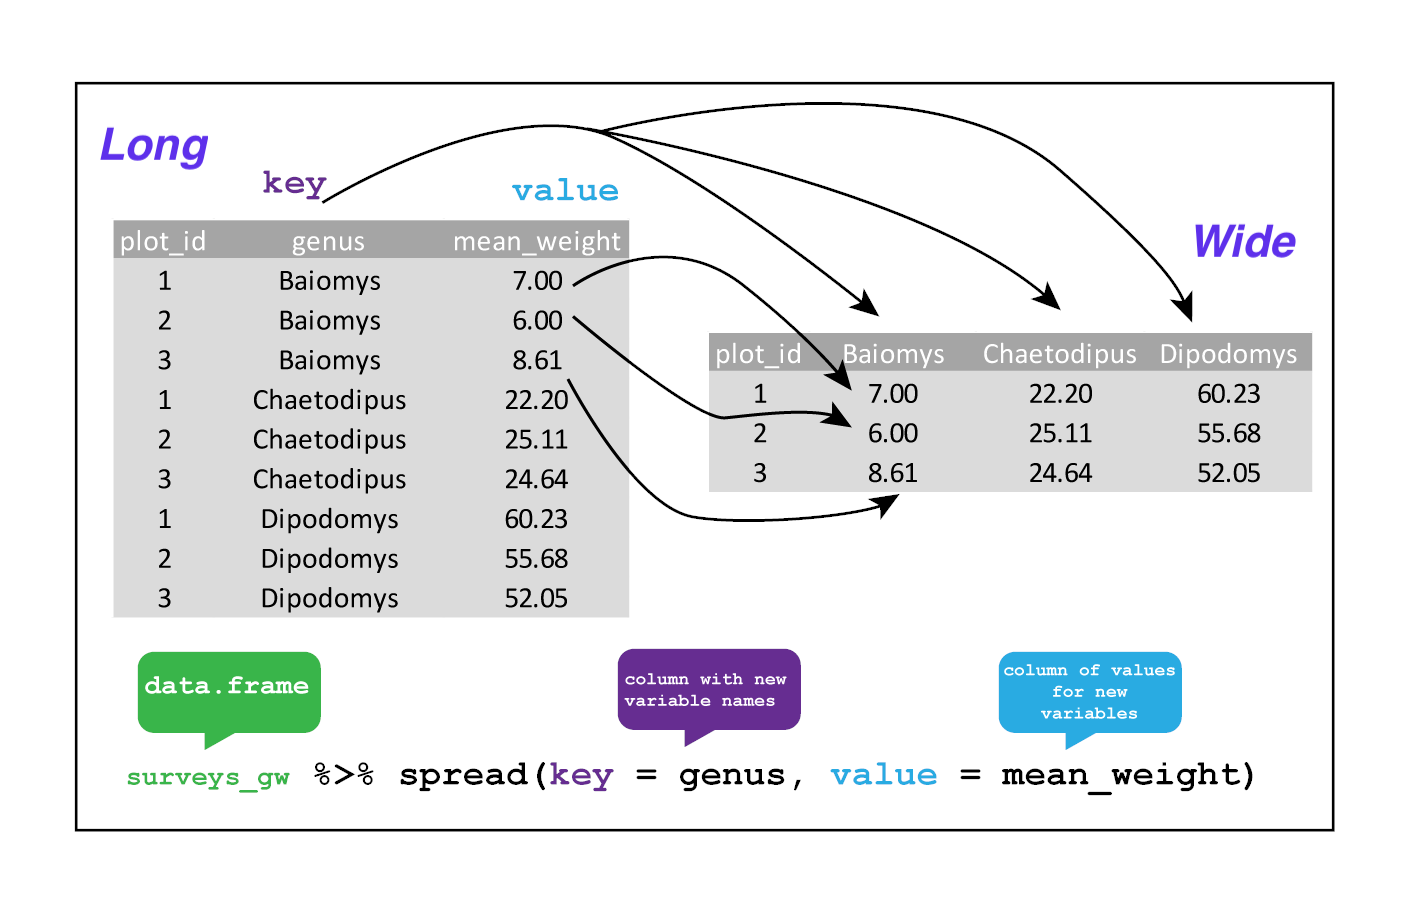
\includegraphics{img/spread_data_R.png}
\caption{}
\end{figure}

We could now plot comparisons between the weight of species in different
plots, although we may wish to fill in the missing values first.

\begin{Shaded}
\begin{Highlighting}[]
\NormalTok{surveys_gw }\OperatorTok
\StringTok{  }\KeywordTok{spread}\NormalTok{(genus, mean_weight, }\DataTypeTok{fill =} \DecValTok{0}\NormalTok{) }\OperatorTok
\StringTok{  }\KeywordTok{head}\NormalTok{()}
\end{Highlighting}
\end{Shaded}

\subsubsection{Gathering}\label{gathering}

The opposing situation could occur if we had been provided with data in
the form of \texttt{surveys\_spread}, where the genus names are column
names, but we wish to treat them as values of a genus variable instead.

In this situation we are gathering the column names and turning them
into a pair of new variables. One variable represents the column names
as values, and the other variable contains the values previously
associated with the column names.

\texttt{gather()} takes four principal arguments:

\begin{enumerate}
\def\labelenumi{\arabic{enumi}.}
\tightlist
\item
  the data
\item
  the \emph{key} column variable we wish to create from column names.
\item
  the \emph{values} column variable we wish to create and fill with
  values associated with the key.
\item
  the names of the columns we use to fill the key variable (or to drop).
\end{enumerate}

To recreate \texttt{surveys\_gw} from \texttt{surveys\_spread} we would
create a key called \texttt{genus} and value called
\texttt{mean\_weight} and use all columns except \texttt{plot\_id} for
the key variable. Here we drop \texttt{plot\_id} column with a minus
sign.

\begin{Shaded}
\begin{Highlighting}[]
\NormalTok{surveys_gather <-}\StringTok{ }\NormalTok{surveys_spread }\OperatorTok
\StringTok{  }\KeywordTok{gather}\NormalTok{(}\DataTypeTok{key =}\NormalTok{ genus, }\DataTypeTok{value =}\NormalTok{ mean_weight, }\OperatorTok{-}\NormalTok{plot_id)}

\KeywordTok{str}\NormalTok{(surveys_gather)}
\end{Highlighting}
\end{Shaded}

\begin{figure}
\centering
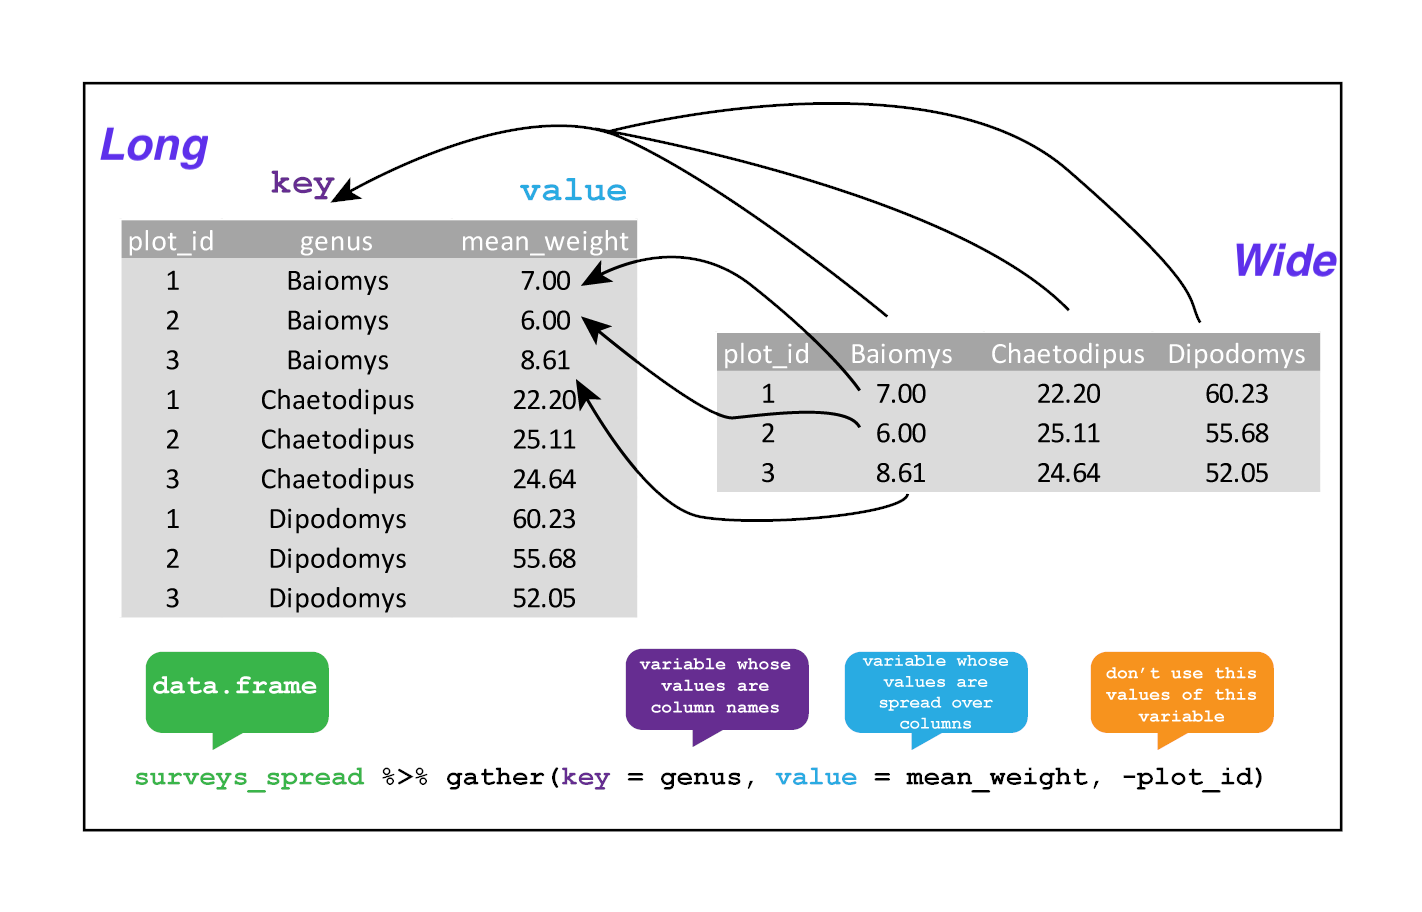
\includegraphics{img/gather_data_R.png}
\caption{}
\end{figure}

Note that now the \texttt{NA} genera are included in the re-gathered
format. Spreading and then gathering can be a useful way to balance out
a dataset so every replicate has the same composition.

We could also have used a specification for what columns to include.
This can be useful if you have a large number of identifying columns,
and it's easier to specify what to gather than what to leave alone. And
if the columns are in a row, we don't even need to list them all out -
just use the \texttt{:} operator!

\begin{Shaded}
\begin{Highlighting}[]
\NormalTok{surveys_spread }\OperatorTok
\StringTok{  }\KeywordTok{gather}\NormalTok{(}\DataTypeTok{key =}\NormalTok{ genus, }\DataTypeTok{value =}\NormalTok{ mean_weight, Baiomys}\OperatorTok{:}\NormalTok{Spermophilus) }\OperatorTok
\StringTok{  }\KeywordTok{head}\NormalTok{()}
\end{Highlighting}
\end{Shaded}

\begin{quote}
\subsection{Challenge}\label{challenge-7}

\begin{enumerate}
\def\labelenumi{\arabic{enumi}.}
\tightlist
\item
  Spread the \texttt{surveys} data frame with \texttt{year} as columns,
  \texttt{plot\_id} as rows, and the number of genera per plot as the
  values. You will need to summarize before reshaping, and use the
  function \texttt{n\_distinct()} to get the number of unique genera
  within a particular chunk of data. It's a powerful function! See
  \texttt{?n\_distinct} for more.
\end{enumerate}

Answer

\begin{Shaded}
\begin{Highlighting}[]
\NormalTok{rich_time <-}\StringTok{ }\NormalTok{surveys }\OperatorTok
\StringTok{  }\KeywordTok{group_by}\NormalTok{(plot_id, year) }\OperatorTok
\StringTok{  }\KeywordTok{summarize}\NormalTok{(}\DataTypeTok{n_genera =} \KeywordTok{n_distinct}\NormalTok{(genus)) }\OperatorTok
\StringTok{  }\KeywordTok{spread}\NormalTok{(year, n_genera)}

\KeywordTok{head}\NormalTok{(rich_time)}
\end{Highlighting}
\end{Shaded}

\begin{enumerate}
\def\labelenumi{\arabic{enumi}.}
\setcounter{enumi}{1}
\tightlist
\item
  Now take that data frame and \texttt{gather()} it again, so each row
  is a unique \texttt{plot\_id} by \texttt{year} combination.
\end{enumerate}

Answer

\begin{Shaded}
\begin{Highlighting}[]
\NormalTok{rich_time }\OperatorTok
\StringTok{  }\KeywordTok{gather}\NormalTok{(year, n_genera, }\OperatorTok{-}\NormalTok{plot_id)}
\end{Highlighting}
\end{Shaded}

\begin{enumerate}
\def\labelenumi{\arabic{enumi}.}
\setcounter{enumi}{2}
\tightlist
\item
  The \texttt{surveys} data set has two measurement columns:
  \texttt{hindfoot\_length} and \texttt{weight}. This makes it difficult
  to do things like look at the relationship between mean values of each
  measurement per year in different plot types. Let's walk through a
  common solution for this type of problem. First, use \texttt{gather()}
  to create a dataset where we have a key column called
  \texttt{measurement} and a \texttt{value} column that takes on the
  value of either \texttt{hindfoot\_length} or \texttt{weight}.
  \emph{Hint}: You'll need to specify which columns are being gathered.
\end{enumerate}

Answer

\begin{Shaded}
\begin{Highlighting}[]
\NormalTok{surveys_long <-}\StringTok{ }\NormalTok{surveys }\OperatorTok
\StringTok{  }\KeywordTok{gather}\NormalTok{(measurement, value, hindfoot_length, weight)}
\end{Highlighting}
\end{Shaded}

\begin{enumerate}
\def\labelenumi{\arabic{enumi}.}
\setcounter{enumi}{3}
\tightlist
\item
  With this new data set, calculate the average of each
  \texttt{measurement} in each \texttt{year} for each different
  \texttt{plot\_type}. Then \texttt{spread()} them into a data set with
  a column for \texttt{hindfoot\_length} and \texttt{weight}.
  \emph{Hint}: You only need to specify the key and value columns for
  \texttt{spread()}.
\end{enumerate}

Answer

\begin{Shaded}
\begin{Highlighting}[]
\NormalTok{surveys_long }\OperatorTok
\StringTok{  }\KeywordTok{group_by}\NormalTok{(year, measurement, plot_type) }\OperatorTok
\StringTok{  }\KeywordTok{summarize}\NormalTok{(}\DataTypeTok{mean_value =} \KeywordTok{mean}\NormalTok{(value, }\DataTypeTok{na.rm=}\OtherTok{TRUE}\NormalTok{)) }\OperatorTok
\StringTok{  }\KeywordTok{spread}\NormalTok{(measurement, mean_value)}
\end{Highlighting}
\end{Shaded}
\end{quote}

\section{Exporting data}\label{exporting-data}

Now that you have learned how to use \textbf{\texttt{dplyr}} to extract
information from or summarize your raw data, you may want to export
these new data sets to share them with your collaborators or for
archival.

Similar to the \texttt{read\_csv()} function used for reading CSV files
into R, there is a \texttt{write\_csv()} function that generates CSV
files from data frames.

\begin{Shaded}
\begin{Highlighting}[]
\KeywordTok{write_csv}\NormalTok{(surveys_spread, }\StringTok{"data/surveys_spread.csv"}\NormalTok{)}
\end{Highlighting}
\end{Shaded}

\section{Factors}\label{factors}

This section is from Jenny Bryan's course at UBC: Stat 545

Factors are the variable type that useRs love to hate. It is how we
store truly categorical information in R. The values a factor can take
on are called the levels. In general, the levels are friendly
human-readable character strings, like ``male/female'' and
``control/treated''. But never ever ever forget that, under the hood, R
is really storing integer codes 1, 2, 3, etc.

This Janus-like nature of factors means they are rich with booby traps
for the unsuspecting but they are a necessary evil. I recommend you
learn how to be the boss of your factors. The pros far outweigh the
cons. Specifically in modelling and figure-making, factors are
anticipated and accommodated by the functions and packages you will want
to exploit.

The worst kind of factor is the stealth factor. The variable that you
think of as character, but that is actually a factor (numeric!!). This
is a classic R gotcha. Check your variable types explicitly when things
seem weird. It happens to the best of us.

Where do stealth factors come from? Base R has a burning desire to turn
character information into factor. The happens most commonly at data
import via read.csv() and friends. But data.frame() and other functions
are also eager to convert character to factor. To shut this down, use
stringsAsFactors = FALSE in read.csv() and data.frame() or -- even
better -- use the tidyverse! For data import, use readr::read\_csv(),
readr::read\_tsv(), etc. For data frame creation, use tibble::tibble().
And so on.

See for yourself the difference in how strings are treated with the two
different methods of reading a csv file.

\begin{Shaded}
\begin{Highlighting}[]
\NormalTok{surveys. <-}\StringTok{ }\KeywordTok{read.csv}\NormalTok{(}\StringTok{"data/surveys.csv"}\NormalTok{)}
\NormalTok{surveys_ <-}\StringTok{ }\KeywordTok{read_csv}\NormalTok{(}\StringTok{"data/surveys.csv"}\NormalTok{)}
\end{Highlighting}
\end{Shaded}

\begin{verbatim}
#> Parsed with column specification:
#> cols(
#>   record_id = col_integer(),
#>   month = col_integer(),
#>   day = col_integer(),
#>   year = col_integer(),
#>   plot_id = col_integer(),
#>   species_id = col_character(),
#>   sex = col_character(),
#>   hindfoot_length = col_integer(),
#>   weight = col_integer()
#> )
\end{verbatim}

\begin{Shaded}
\begin{Highlighting}[]
\KeywordTok{str}\NormalTok{(surveys.)}
\KeywordTok{str}\NormalTok{(surveys_)}
\end{Highlighting}
\end{Shaded}

\subsection{The forcats Package}\label{the-forcats-package}

forcats is a core package in the tidyverse. It is installed via
\texttt{install.packages("tidyverse")} and attached via
\texttt{library(tidyverse)}. You can always load it individually via
\texttt{library(forcats)}. Main functions start with fct\_. There really
is no coherent family of base functions that forcats replaces -- that's
why it's such a welcome addition.

\begin{Shaded}
\begin{Highlighting}[]
\KeywordTok{library}\NormalTok{(tidyverse)}
\KeywordTok{library}\NormalTok{(forcats)}


\KeywordTok{library}\NormalTok{(gapminder)}
\end{Highlighting}
\end{Shaded}

Get to know your factor before you start touching it! It's polite. Let's
use gapminder\$continent as our example.

\begin{Shaded}
\begin{Highlighting}[]
\KeywordTok{str}\NormalTok{(gapminder}\OperatorTok{$}\NormalTok{continent)}
\KeywordTok{levels}\NormalTok{(gapminder}\OperatorTok{$}\NormalTok{continent)}
\KeywordTok{nlevels}\NormalTok{(gapminder}\OperatorTok{$}\NormalTok{continent)}
\KeywordTok{class}\NormalTok{(gapminder}\OperatorTok{$}\NormalTok{continent)}
\end{Highlighting}
\end{Shaded}

To get a frequency table as a tibble, from a tibble, use dplyr::count().
To get similar from a free-range factor, use forcats::fct\_count().

\begin{Shaded}
\begin{Highlighting}[]
\NormalTok{gapminder }\OperatorTok\StringTok{ }
\StringTok{  }\KeywordTok{count}\NormalTok{(continent)}

\KeywordTok{fct_count}\NormalTok{(gapminder}\OperatorTok{$}\NormalTok{continent)}
\end{Highlighting}
\end{Shaded}

\subsubsection{Dropping unused levels:}\label{dropping-unused-levels}

Just because you drop all the rows corresponding to a specific factor
level, the levels of the factor itself do not change. Sometimes all
these unused levels can come back to haunt you later, e.g., in figure
legends.

Watch what happens to the levels of country (= nothing) when we filter
Gapminder to a handful of countries.

\begin{Shaded}
\begin{Highlighting}[]
\KeywordTok{nlevels}\NormalTok{(gapminder}\OperatorTok{$}\NormalTok{country)}

\NormalTok{h_countries <-}\StringTok{ }\KeywordTok{c}\NormalTok{(}\StringTok{"Egypt"}\NormalTok{, }\StringTok{"Haiti"}\NormalTok{, }\StringTok{"Romania"}\NormalTok{, }\StringTok{"Thailand"}\NormalTok{, }\StringTok{"Venezuela"}\NormalTok{)}

\NormalTok{h_gap <-}\StringTok{ }\NormalTok{gapminder }\OperatorTok
\StringTok{  }\KeywordTok{filter}\NormalTok{(country }\OperatorTok\StringTok{ }\NormalTok{h_countries)}

\KeywordTok{nlevels}\NormalTok{(h_gap}\OperatorTok{$}\NormalTok{country)}
\end{Highlighting}
\end{Shaded}

Even though \texttt{h\_gap} only has data for a handful of countries, we
are still schlepping around all 142 levels from the original gapminder
tibble.

How can you get rid of them? The base function \texttt{droplevels()}
operates on all the factors in a data frame or on a single factor. The
function \texttt{forcats::fct\_drop()} operates on a factor.

\begin{Shaded}
\begin{Highlighting}[]
\NormalTok{h_gap_dropped <-}\StringTok{ }\NormalTok{h_gap }\OperatorTok\StringTok{ }
\StringTok{  }\KeywordTok{droplevels}\NormalTok{()}
\KeywordTok{nlevels}\NormalTok{(h_gap_dropped}\OperatorTok{$}\NormalTok{country)}

\NormalTok{h_gap}\OperatorTok{$}\NormalTok{country }\OperatorTok
\StringTok{  }\KeywordTok{fct_drop}\NormalTok{() }\OperatorTok
\StringTok{  }\KeywordTok{levels}\NormalTok{()}
\end{Highlighting}
\end{Shaded}

\subsubsection{Change order of the levels,
principled}\label{change-order-of-the-levels-principled}

By default, factor levels are ordered alphabetically. Which might as
well be random, when you think about it! It is preferable to order the
levels according to some principle:

\begin{itemize}
\tightlist
\item
  Frequency.Make the most common level the first and so on.
\item
  Another variable. Order factor levels according to a summary statistic
  for another variable. Example: order Gapminder countries by life
  expectancy.
\end{itemize}

First, let's order continent by frequency, forwards and backwards. This
is often a great idea for tables and figures, esp. frequency barplots.

\begin{Shaded}
\begin{Highlighting}[]
\NormalTok{## default order is alphabetical}
\NormalTok{gapminder}\OperatorTok{$}\NormalTok{continent }\OperatorTok
\StringTok{  }\KeywordTok{levels}\NormalTok{()}

\NormalTok{## order by frequency}
\NormalTok{gapminder}\OperatorTok{$}\NormalTok{continent }\OperatorTok\StringTok{ }
\StringTok{  }\KeywordTok{fct_infreq}\NormalTok{() }\OperatorTok
\StringTok{  }\KeywordTok{levels}\NormalTok{()}

\NormalTok{## backwards!}
\NormalTok{gapminder}\OperatorTok{$}\NormalTok{continent }\OperatorTok\StringTok{ }
\StringTok{  }\KeywordTok{fct_infreq}\NormalTok{() }\OperatorTok
\StringTok{  }\KeywordTok{fct_rev}\NormalTok{() }\OperatorTok\StringTok{ }
\StringTok{  }\KeywordTok{levels}\NormalTok{()}

\NormalTok{## order countries by median life expectancy}
\KeywordTok{fct_reorder}\NormalTok{(gapminder}\OperatorTok{$}\NormalTok{country, gapminder}\OperatorTok{$}\NormalTok{lifeExp) }\OperatorTok\StringTok{ }
\StringTok{  }\KeywordTok{levels}\NormalTok{() }\OperatorTok\StringTok{ }\KeywordTok{head}\NormalTok{()}
\end{Highlighting}
\end{Shaded}

\subsubsection{\texorpdfstring{Change order of the levels, ``because I
said
so''}{Change order of the levels, because I said so}}\label{change-order-of-the-levels-because-i-said-so}

Sometimes you just want to hoist one or more levels to the front. Why?
Because I said so.

\begin{Shaded}
\begin{Highlighting}[]
\NormalTok{h_gap}\OperatorTok{$}\NormalTok{country }\OperatorTok\StringTok{ }\KeywordTok{levels}\NormalTok{()}

\NormalTok{h_gap}\OperatorTok{$}\NormalTok{country }\OperatorTok\StringTok{ }\KeywordTok{fct_relevel}\NormalTok{(}\StringTok{"Romania"}\NormalTok{, }\StringTok{"Haiti"}\NormalTok{) }\OperatorTok\StringTok{ }\KeywordTok{levels}\NormalTok{()}
\end{Highlighting}
\end{Shaded}

This might be useful if you are preparing a report for, say, the
Romanian government. The reason for always putting Romania first has
nothing to do with the data, it is important for external reasons and
you need a way to express this.

\subsubsection{Recode the levels}\label{recode-the-levels}

Sometimes you have better ideas about what certain levels should be.
This is called recoding.

\begin{Shaded}
\begin{Highlighting}[]
\NormalTok{i_gap <-}\StringTok{ }\NormalTok{gapminder }\OperatorTok\StringTok{ }
\StringTok{  }\KeywordTok{filter}\NormalTok{(country }\OperatorTok\StringTok{ }\KeywordTok{c}\NormalTok{(}\StringTok{"United States"}\NormalTok{, }\StringTok{"Sweden"}\NormalTok{, }\StringTok{"Australia"}\NormalTok{)) }\OperatorTok\StringTok{ }
\StringTok{  }\KeywordTok{droplevels}\NormalTok{()}

\NormalTok{i_gap}\OperatorTok{$}\NormalTok{country }\OperatorTok\StringTok{ }\KeywordTok{levels}\NormalTok{()}

\NormalTok{i_gap}\OperatorTok{$}\NormalTok{country }\OperatorTok
\StringTok{  }\KeywordTok{fct_recode}\NormalTok{(}\StringTok{"USA"}\NormalTok{ =}\StringTok{ "United States"}\NormalTok{, }\StringTok{"Oz"}\NormalTok{ =}\StringTok{ "Australia"}\NormalTok{) }\OperatorTok\StringTok{ }\KeywordTok{levels}\NormalTok{()}
\end{Highlighting}
\end{Shaded}

Exercise: Isolate the data for ``Australia'', ``Korea, Dem. Rep.'', and
``Korea, Rep.'' in the 2000x. Revalue the country factor levels to
``Oz'', ``North Korea'', and ``South Korea''.

\begin{center}\rule{0.5\linewidth}{\linethickness}\end{center}

\begin{quote}
\subsection{Learning Objectives}\label{learning-objectives-4}

\begin{itemize}
\tightlist
\item
  Produce scatter plots, boxplots, and time series plots using ggplot.
\item
  Set universal plot settings.
\item
  Describe what faceting is and apply faceting in ggplot.
\item
  Modify the aesthetics of an existing ggplot plot (including axis
  labels and color).
\item
  Build complex and customized plots from data in a data frame.
\end{itemize}
\end{quote}

\begin{center}\rule{0.5\linewidth}{\linethickness}\end{center}

\chapter{Data Viz: ggplot2}\label{data-viz-ggplot2}

We start by loading the required packages. \textbf{\texttt{ggplot2}} is
included in the \textbf{\texttt{tidyverse}} package.

\begin{Shaded}
\begin{Highlighting}[]
\KeywordTok{library}\NormalTok{(tidyverse)}
\end{Highlighting}
\end{Shaded}

If not still in the workspace, load the data we saved in the previous
lesson.

\begin{Shaded}
\begin{Highlighting}[]
\NormalTok{surveys_complete <-}\StringTok{ }\KeywordTok{read_csv}\NormalTok{(}\StringTok{"data_output/surveys_complete.csv"}\NormalTok{)}
\end{Highlighting}
\end{Shaded}

\section{\texorpdfstring{Plotting with
\textbf{\texttt{ggplot2}}}{Plotting with ggplot2}}\label{plotting-with-ggplot2}

\textbf{\texttt{ggplot2}} is a plotting package that makes it simple to
create complex plots from data in a data frame. It provides a more
programmatic interface for specifying what variables to plot, how they
are displayed, and general visual properties. Therefore, we only need
minimal changes if the underlying data change or if we decide to change
from a bar plot to a scatterplot. This helps in creating publication
quality plots with minimal amounts of adjustments and tweaking.

\textbf{\texttt{ggplot2}} functions like data in the `long' format,
i.e., a column for every dimension, and a row for every observation.
Well-structured data will save you lots of time when making figures with
\textbf{\texttt{ggplot2}}

ggplot graphics are built step by step by adding new elements. Adding
layers in this fashion allows for extensive flexibility and
customization of plots.

To build a ggplot, we will use the following basic template that can be
used for different types of plots:

\begin{verbatim}
ggplot(data = <DATA>, mapping = aes(<MAPPINGS>)) +  <GEOM_FUNCTION>()
\end{verbatim}

\begin{itemize}
\tightlist
\item
  use the \texttt{ggplot()} function and bind the plot to a specific
  data frame using the \texttt{data} argument
\end{itemize}

\begin{Shaded}
\begin{Highlighting}[]
\KeywordTok{ggplot}\NormalTok{(}\DataTypeTok{data =}\NormalTok{ surveys_complete)}
\end{Highlighting}
\end{Shaded}

\begin{itemize}
\tightlist
\item
  define a mapping (using the aesthetic (\texttt{aes}) function), by
  selecting the variables to be plotted and specifying how to present
  them in the graph, e.g.~as x/y positions or characteristics such as
  size, shape, color, etc.
\end{itemize}

\begin{Shaded}
\begin{Highlighting}[]
\KeywordTok{ggplot}\NormalTok{(}\DataTypeTok{data =}\NormalTok{ surveys_complete, }\DataTypeTok{mapping =} \KeywordTok{aes}\NormalTok{(}\DataTypeTok{x =}\NormalTok{ weight, }\DataTypeTok{y =}\NormalTok{ hindfoot_length))}
\end{Highlighting}
\end{Shaded}

\begin{itemize}
\item
  add `geoms' -- graphical representations of the data in the plot
  (points, lines, bars). \textbf{\texttt{ggplot2}} offers many different
  geoms; we will use some common ones today, including:

  \begin{itemize}
  \tightlist
  \item
    \texttt{geom\_point()} for scatter plots, dot plots, etc.
  \item
    \texttt{geom\_boxplot()} for, well, boxplots!
  \item
    \texttt{geom\_line()} for trend lines, time series, etc.
  \end{itemize}
\end{itemize}

To add a geom to the plot use the \texttt{+} operator. Because we have
two continuous variables, let's use \texttt{geom\_point()} first:

\begin{Shaded}
\begin{Highlighting}[]
\KeywordTok{ggplot}\NormalTok{(}\DataTypeTok{data =}\NormalTok{ surveys_complete, }\DataTypeTok{mapping =} \KeywordTok{aes}\NormalTok{(}\DataTypeTok{x =}\NormalTok{ weight, }\DataTypeTok{y =}\NormalTok{ hindfoot_length)) }\OperatorTok{+}
\StringTok{  }\KeywordTok{geom_point}\NormalTok{()}
\end{Highlighting}
\end{Shaded}

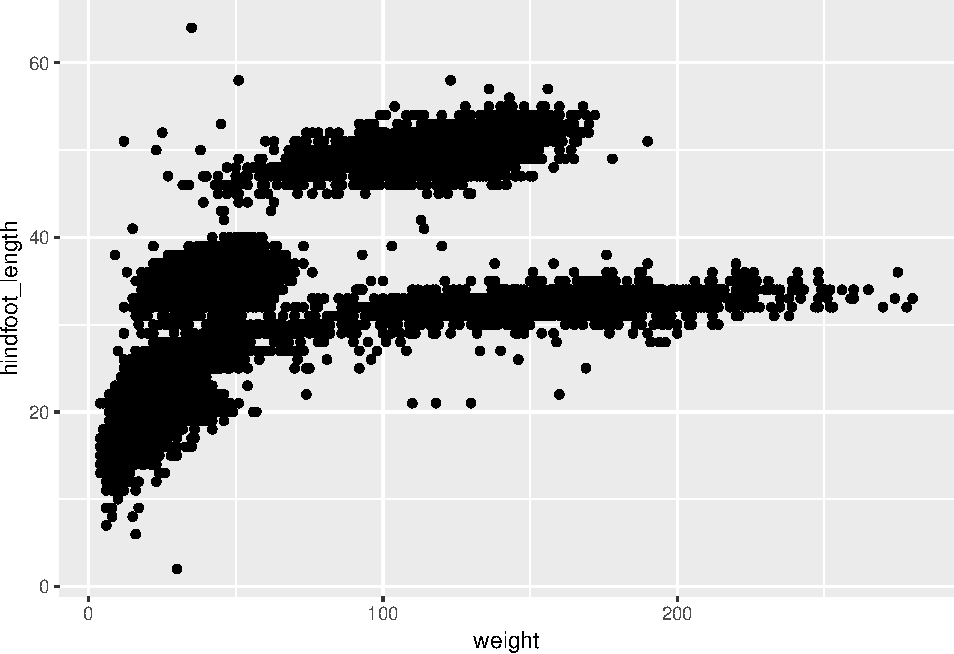
\includegraphics{img/R-ecology-first-ggplot-1.pdf}

The \texttt{+} in the \textbf{\texttt{ggplot2}} package is particularly
useful because it allows you to modify existing \texttt{ggplot} objects.
This means you can easily set up plot templates and conveniently explore
different types of plots, so the above plot can also be generated with
code like this:

\begin{Shaded}
\begin{Highlighting}[]
\CommentTok{# Assign plot to a variable}
\NormalTok{surveys_plot <-}\StringTok{ }\KeywordTok{ggplot}\NormalTok{(}\DataTypeTok{data =}\NormalTok{ surveys_complete, }
                       \DataTypeTok{mapping =} \KeywordTok{aes}\NormalTok{(}\DataTypeTok{x =}\NormalTok{ weight, }\DataTypeTok{y =}\NormalTok{ hindfoot_length))}

\CommentTok{# Draw the plot}
\NormalTok{surveys_plot }\OperatorTok{+}\StringTok{ }
\StringTok{    }\KeywordTok{geom_point}\NormalTok{()}
\end{Highlighting}
\end{Shaded}

\textbf{Notes}

\begin{itemize}
\tightlist
\item
  Anything you put in the \texttt{ggplot()} function can be seen by any
  geom layers that you add (i.e., these are universal plot settings).
  This includes the x- and y-axis mapping you set up in \texttt{aes()}.
\item
  You can also specify mappings for a given geom independently of the
  mappings defined globally in the \texttt{ggplot()} function.
\item
  The \texttt{+} sign used to add new layers must be placed at the end
  of the line containing the \emph{previous} layer. If, instead, the
  \texttt{+} sign is added at the beginning of the line containing the
  new layer, \textbf{\texttt{ggplot2}} will not add the new layer and
  will return an error message.
\end{itemize}

\begin{Shaded}
\begin{Highlighting}[]
\CommentTok{# This is the correct syntax for adding layers}
\NormalTok{surveys_plot }\OperatorTok{+}
\StringTok{  }\KeywordTok{geom_point}\NormalTok{()}

\CommentTok{# This will not add the new layer and will return an error message}
\NormalTok{surveys_plot}
  \OperatorTok{+}\StringTok{ }\KeywordTok{geom_point}\NormalTok{()}
\end{Highlighting}
\end{Shaded}

\section{Building your plots
iteratively}\label{building-your-plots-iteratively}

Building plots with \textbf{\texttt{ggplot2}} is typically an iterative
process. We start by defining the dataset we'll use, lay out the axes,
and choose a geom:

\begin{Shaded}
\begin{Highlighting}[]
\KeywordTok{ggplot}\NormalTok{(}\DataTypeTok{data =}\NormalTok{ surveys_complete, }\DataTypeTok{mapping =} \KeywordTok{aes}\NormalTok{(}\DataTypeTok{x =}\NormalTok{ weight, }\DataTypeTok{y =}\NormalTok{ hindfoot_length)) }\OperatorTok{+}
\StringTok{    }\KeywordTok{geom_point}\NormalTok{()}
\end{Highlighting}
\end{Shaded}

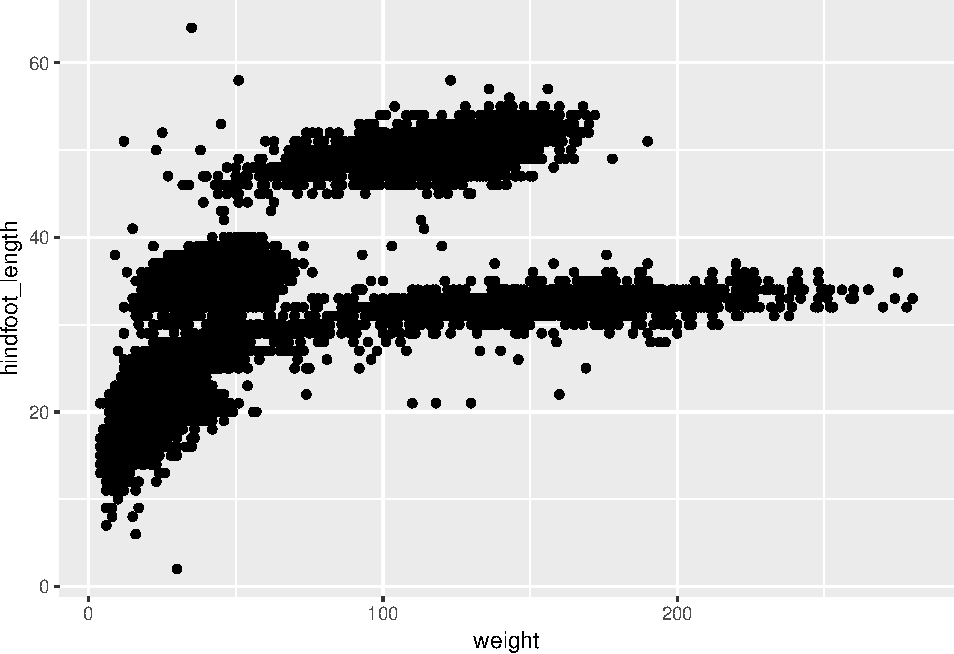
\includegraphics{img/R-ecology-create-ggplot-object-1.pdf}

Then, we start modifying this plot to extract more information from it.
For instance, we can add transparency (\texttt{alpha}) to avoid
overplotting:

\begin{Shaded}
\begin{Highlighting}[]
\KeywordTok{ggplot}\NormalTok{(}\DataTypeTok{data =}\NormalTok{ surveys_complete, }\DataTypeTok{mapping =} \KeywordTok{aes}\NormalTok{(}\DataTypeTok{x =}\NormalTok{ weight, }\DataTypeTok{y =}\NormalTok{ hindfoot_length)) }\OperatorTok{+}
\StringTok{    }\KeywordTok{geom_point}\NormalTok{(}\DataTypeTok{alpha =} \FloatTok{0.1}\NormalTok{)}
\end{Highlighting}
\end{Shaded}

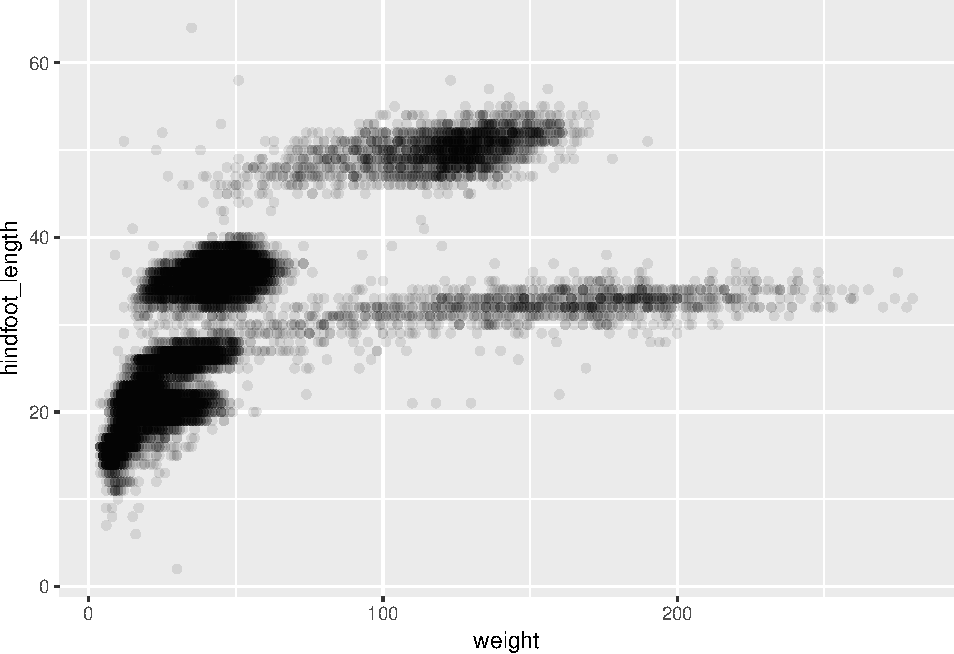
\includegraphics{img/R-ecology-adding-transparency-1.pdf}

We can also add colors for all the points:

\begin{Shaded}
\begin{Highlighting}[]
\KeywordTok{ggplot}\NormalTok{(}\DataTypeTok{data =}\NormalTok{ surveys_complete, }\DataTypeTok{mapping =} \KeywordTok{aes}\NormalTok{(}\DataTypeTok{x =}\NormalTok{ weight, }\DataTypeTok{y =}\NormalTok{ hindfoot_length)) }\OperatorTok{+}
\StringTok{    }\KeywordTok{geom_point}\NormalTok{(}\DataTypeTok{alpha =} \FloatTok{0.1}\NormalTok{, }\DataTypeTok{color =} \StringTok{"blue"}\NormalTok{)}
\end{Highlighting}
\end{Shaded}

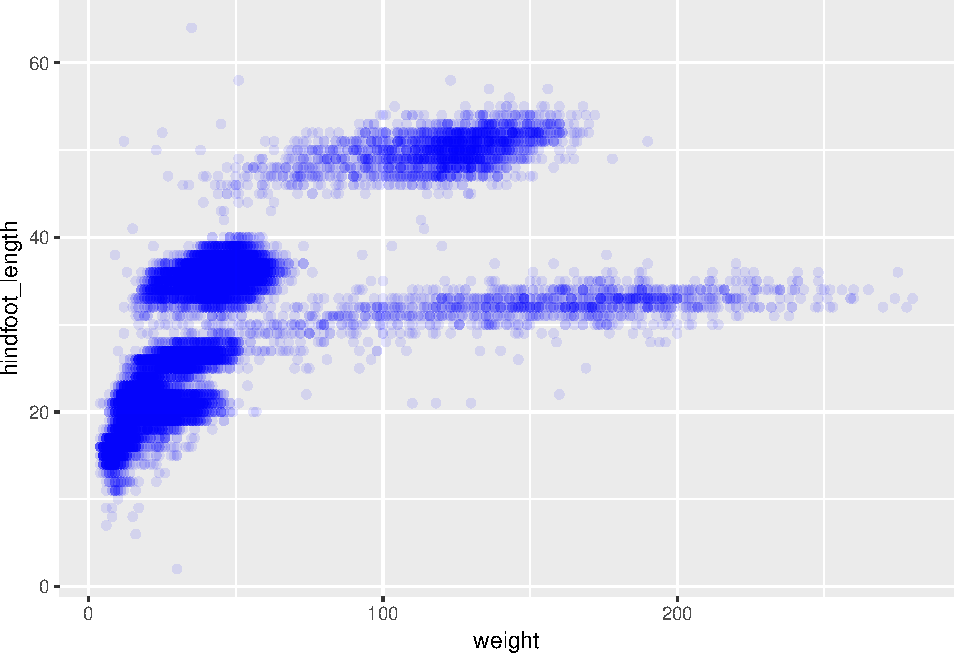
\includegraphics{img/R-ecology-adding-colors-1.pdf}

Or to color each species in the plot differently, you could use a vector
as an input to the argument \textbf{color}. \textbf{\texttt{ggplot2}}
will provide a different color corresponding to different values in the
vector. Here is an example where we color with
\textbf{\texttt{species\_id}}:

\begin{Shaded}
\begin{Highlighting}[]
\KeywordTok{ggplot}\NormalTok{(}\DataTypeTok{data =}\NormalTok{ surveys_complete, }\DataTypeTok{mapping =} \KeywordTok{aes}\NormalTok{(}\DataTypeTok{x =}\NormalTok{ weight, }\DataTypeTok{y =}\NormalTok{ hindfoot_length)) }\OperatorTok{+}
\StringTok{    }\KeywordTok{geom_point}\NormalTok{(}\DataTypeTok{alpha =} \FloatTok{0.1}\NormalTok{, }\KeywordTok{aes}\NormalTok{(}\DataTypeTok{color =}\NormalTok{ species_id))}
\end{Highlighting}
\end{Shaded}

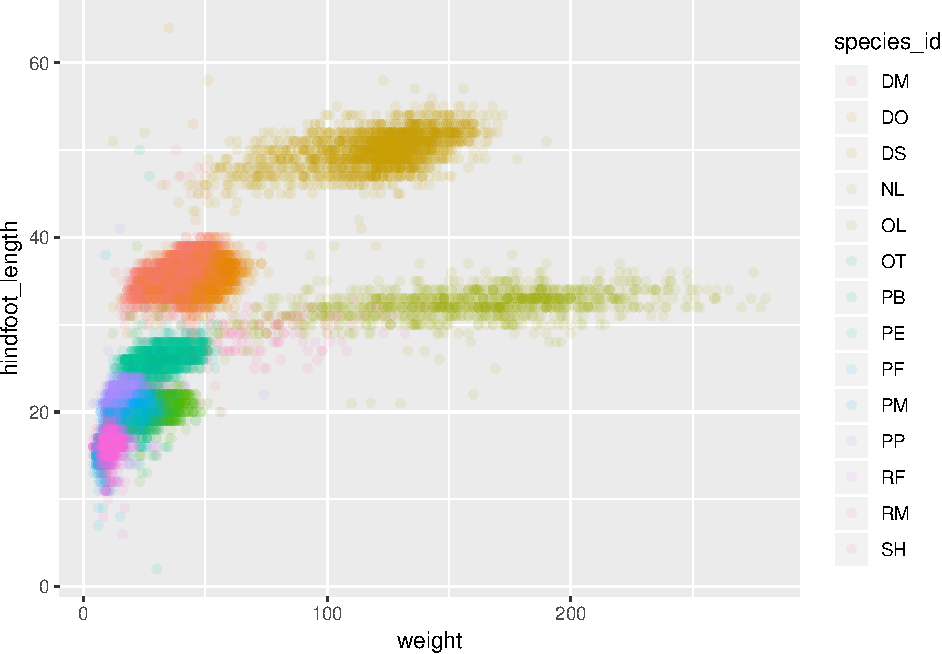
\includegraphics{img/R-ecology-color-1.pdf}

We can also specify the colors directly inside the mapping provided in
the \texttt{ggplot()} function. This will be seen by any geom layers and
the mapping will be determined by the x- and y-axis set up in
\texttt{aes()}.

\begin{Shaded}
\begin{Highlighting}[]
\KeywordTok{ggplot}\NormalTok{(}\DataTypeTok{data =}\NormalTok{ surveys_complete, }\DataTypeTok{mapping =} \KeywordTok{aes}\NormalTok{(}\DataTypeTok{x =}\NormalTok{ weight, }\DataTypeTok{y =}\NormalTok{ hindfoot_length, }\DataTypeTok{color =}\NormalTok{ species_id)) }\OperatorTok{+}
\StringTok{    }\KeywordTok{geom_point}\NormalTok{(}\DataTypeTok{alpha =} \FloatTok{0.1}\NormalTok{)}
\end{Highlighting}
\end{Shaded}

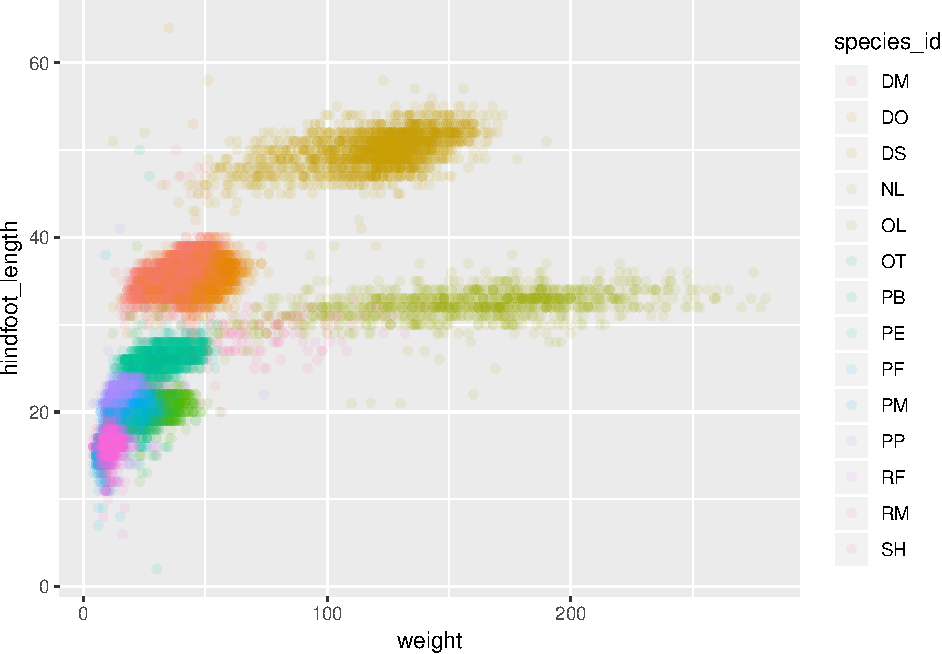
\includegraphics{img/R-ecology-color-by-species1-1.pdf}

Notice that we can change the geom layer and colors will be still
determined by \textbf{\texttt{species\_id}}

\begin{Shaded}
\begin{Highlighting}[]
\KeywordTok{ggplot}\NormalTok{(}\DataTypeTok{data =}\NormalTok{ surveys_complete, }\DataTypeTok{mapping =} \KeywordTok{aes}\NormalTok{(}\DataTypeTok{x =}\NormalTok{ weight, }\DataTypeTok{y =}\NormalTok{ hindfoot_length, }\DataTypeTok{color =}\NormalTok{ species_id)) }\OperatorTok{+}
\StringTok{    }\KeywordTok{geom_jitter}\NormalTok{(}\DataTypeTok{alpha =} \FloatTok{0.1}\NormalTok{)}
\end{Highlighting}
\end{Shaded}

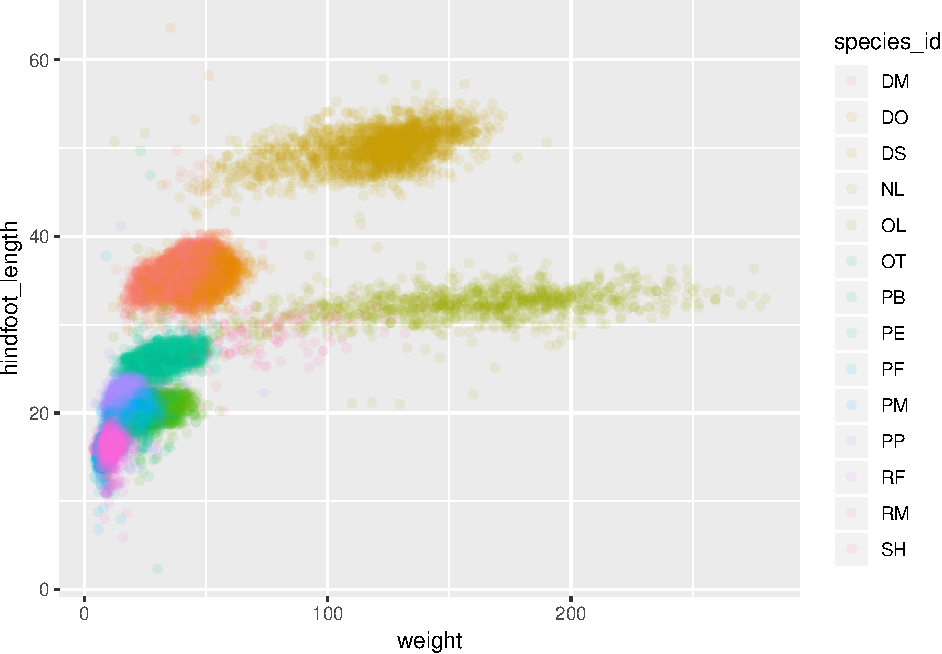
\includegraphics{img/R-ecology-color-by-species2-1.pdf}

\begin{quote}
\subsection{Challenge}\label{challenge-8}

Use what you just learned to create a scatter plot of \texttt{weight}
over \texttt{species\_id} with the plot types showing in different
colors. Is this a good way to show this type of data?

Answer

\begin{Shaded}
\begin{Highlighting}[]
\KeywordTok{ggplot}\NormalTok{(}\DataTypeTok{data =}\NormalTok{ surveys_complete, }\DataTypeTok{mapping =} \KeywordTok{aes}\NormalTok{(}\DataTypeTok{x =}\NormalTok{ species_id, }\DataTypeTok{y =}\NormalTok{ weight)) }\OperatorTok{+}
\StringTok{   }\KeywordTok{geom_point}\NormalTok{(}\KeywordTok{aes}\NormalTok{(}\DataTypeTok{color =}\NormalTok{ plot_type))}
\end{Highlighting}
\end{Shaded}

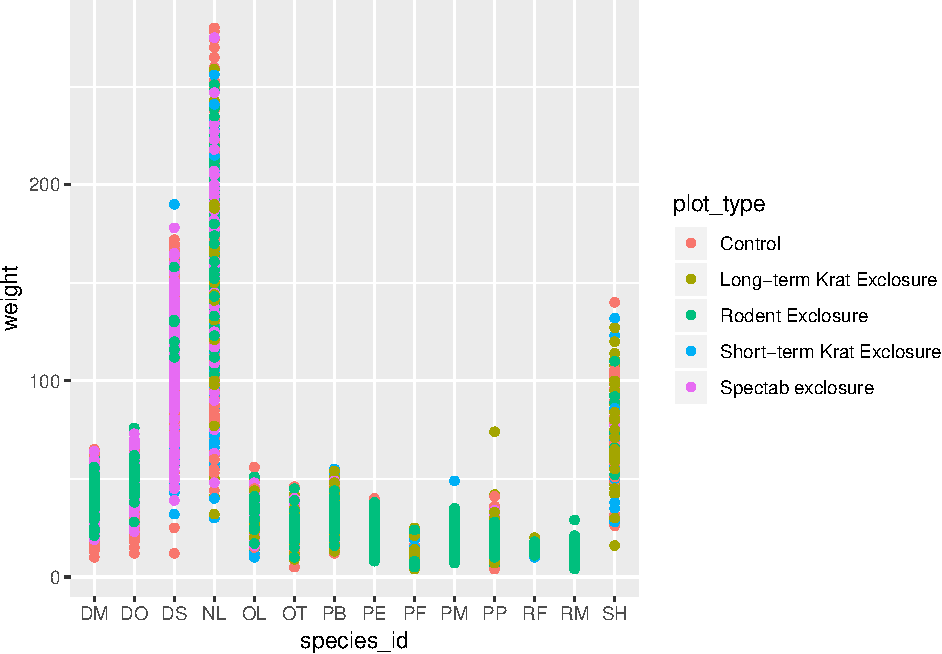
\includegraphics{img/R-ecology-scatter-challenge-1.pdf}
\end{quote}

\section{Boxplot}\label{boxplot}

We can use boxplots to visualize the distribution of weight within each
species:

\begin{Shaded}
\begin{Highlighting}[]
\KeywordTok{ggplot}\NormalTok{(}\DataTypeTok{data =}\NormalTok{ surveys_complete, }\DataTypeTok{mapping =} \KeywordTok{aes}\NormalTok{(}\DataTypeTok{x =}\NormalTok{ species_id, }\DataTypeTok{y =}\NormalTok{ weight)) }\OperatorTok{+}
\StringTok{    }\KeywordTok{geom_boxplot}\NormalTok{()}
\end{Highlighting}
\end{Shaded}

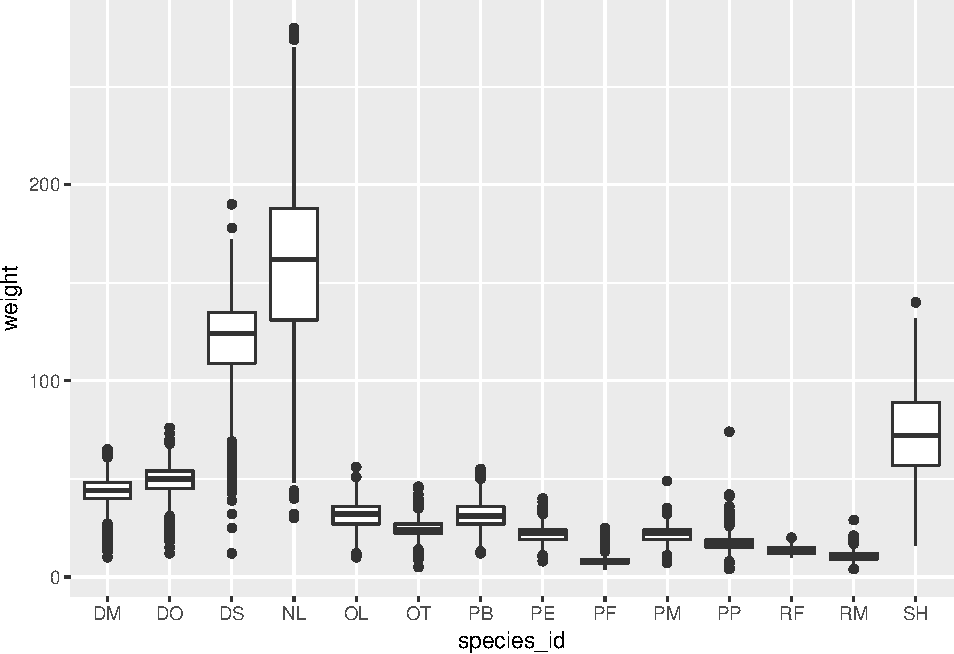
\includegraphics{img/R-ecology-boxplot-1.pdf}

By adding points to boxplot, we can have a better idea of the number of
measurements and of their distribution:

\begin{Shaded}
\begin{Highlighting}[]
\KeywordTok{ggplot}\NormalTok{(}\DataTypeTok{data =}\NormalTok{ surveys_complete, }\DataTypeTok{mapping =} \KeywordTok{aes}\NormalTok{(}\DataTypeTok{x =}\NormalTok{ species_id, }\DataTypeTok{y =}\NormalTok{ weight)) }\OperatorTok{+}
\StringTok{    }\KeywordTok{geom_boxplot}\NormalTok{(}\DataTypeTok{alpha =} \DecValTok{0}\NormalTok{) }\OperatorTok{+}
\StringTok{    }\KeywordTok{geom_jitter}\NormalTok{(}\DataTypeTok{alpha =} \FloatTok{0.3}\NormalTok{, }\DataTypeTok{color =} \StringTok{"tomato"}\NormalTok{)}
\end{Highlighting}
\end{Shaded}

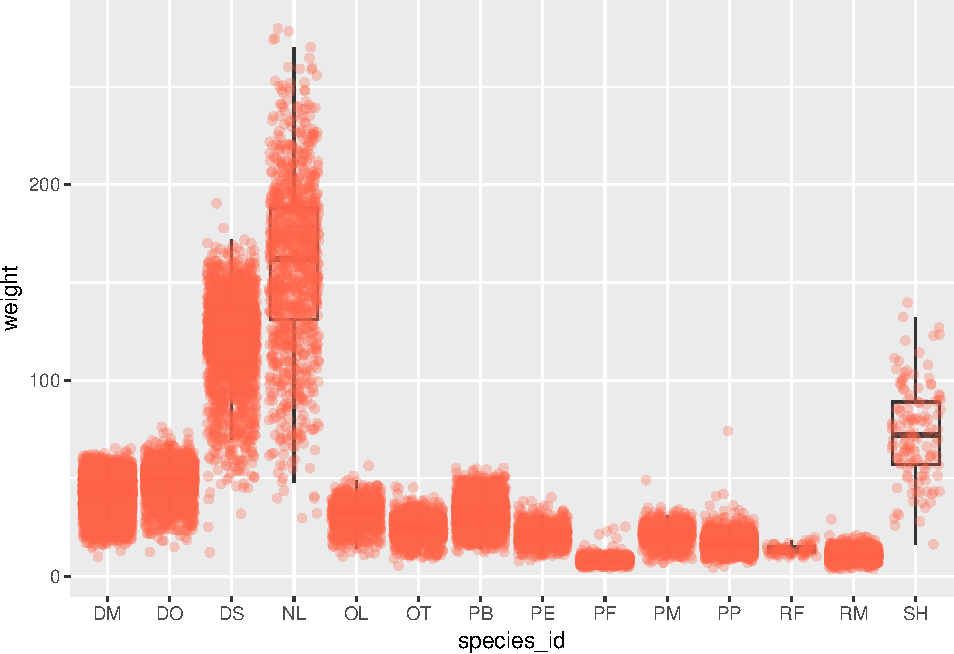
\includegraphics{img/R-ecology-boxplot-with-points-1.pdf}

Notice how the boxplot layer is behind the jitter layer? What do you
need to change in the code to put the boxplot in front of the points
such that it's not hidden?

\begin{quote}
\subsection{Challenges}\label{challenges}

Boxplots are useful summaries, but hide the \emph{shape} of the
distribution. For example, if the distribution is bimodal, we would not
see it in a boxplot. An alternative to the boxplot is the violin plot,
where the shape (of the density of points) is drawn.

\begin{itemize}
\tightlist
\item
  Replace the box plot with a violin plot; see \texttt{geom\_violin()}.
\end{itemize}

In many types of data, it is important to consider the \emph{scale} of
the observations. For example, it may be worth changing the scale of the
axis to better distribute the observations in the space of the plot.
Changing the scale of the axes is done similarly to adding/modifying
other components (i.e., by incrementally adding commands). Try making
these modifications:

\begin{itemize}
\tightlist
\item
  Represent weight on the log\textsubscript{10} scale; see
  \texttt{scale\_y\_log10()}.
\end{itemize}

So far, we've looked at the distribution of weight within species. Try
making a new plot to explore the distribution of another variable within
each species.

\begin{itemize}
\item
  Create a boxplot for \texttt{hindfoot\_length}. Overlay the boxplot
  layer on a jitter layer to show actual measurements.
\item
  Add color to the data points on your boxplot according to the plot
  from which the sample was taken (\texttt{plot\_id}).
\end{itemize}

\emph{Hint:} Check the class for \texttt{plot\_id}. Consider changing
the class of \texttt{plot\_id} from integer to factor. Why does this
change how R makes the graph?
\end{quote}

\section{Plotting time series data}\label{plotting-time-series-data}

Let's calculate number of counts per year for each species. First we
need to group the data and count records within each group:

\begin{Shaded}
\begin{Highlighting}[]
\NormalTok{yearly_counts <-}\StringTok{ }\NormalTok{surveys_complete }\OperatorTok
\StringTok{                 }\KeywordTok{count}\NormalTok{(year, species_id)}
\end{Highlighting}
\end{Shaded}

Time series data can be visualized as a line plot with years on the x
axis and counts on the y axis:

\begin{Shaded}
\begin{Highlighting}[]
\KeywordTok{ggplot}\NormalTok{(}\DataTypeTok{data =}\NormalTok{ yearly_counts, }\DataTypeTok{mapping =} \KeywordTok{aes}\NormalTok{(}\DataTypeTok{x =}\NormalTok{ year, }\DataTypeTok{y =}\NormalTok{ n)) }\OperatorTok{+}
\StringTok{     }\KeywordTok{geom_line}\NormalTok{()}
\end{Highlighting}
\end{Shaded}

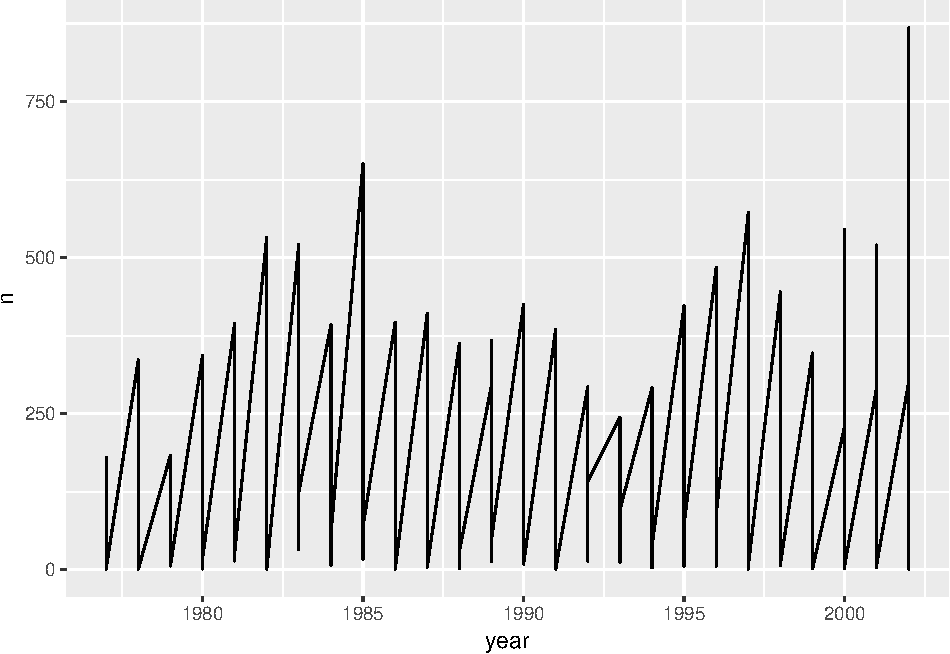
\includegraphics{img/R-ecology-first-time-series-1.pdf}

Unfortunately, this does not work because we plotted data for all the
species together. We need to tell ggplot to draw a line for each species
by modifying the aesthetic function to include
\texttt{group\ =\ species\_id}:

\begin{Shaded}
\begin{Highlighting}[]
\KeywordTok{ggplot}\NormalTok{(}\DataTypeTok{data =}\NormalTok{ yearly_counts, }\DataTypeTok{mapping =} \KeywordTok{aes}\NormalTok{(}\DataTypeTok{x =}\NormalTok{ year, }\DataTypeTok{y =}\NormalTok{ n, }\DataTypeTok{group =}\NormalTok{ species_id)) }\OperatorTok{+}
\StringTok{    }\KeywordTok{geom_line}\NormalTok{()}
\end{Highlighting}
\end{Shaded}

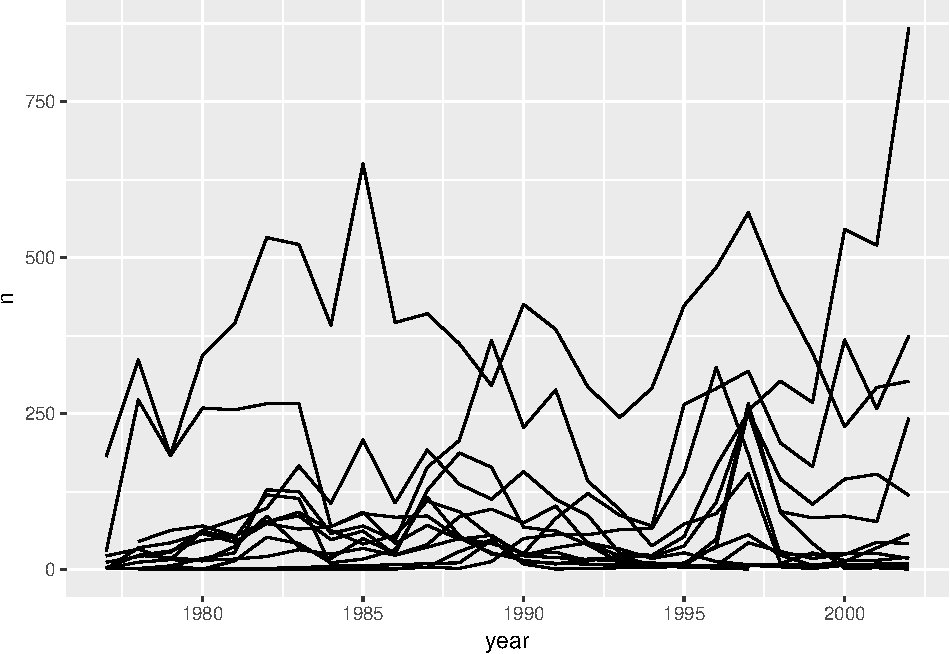
\includegraphics{img/R-ecology-time-series-by-species-1.pdf}

We will be able to distinguish species in the plot if we add colors
(using \texttt{color} also automatically groups the data):

\begin{Shaded}
\begin{Highlighting}[]
\KeywordTok{ggplot}\NormalTok{(}\DataTypeTok{data =}\NormalTok{ yearly_counts, }\DataTypeTok{mapping =} \KeywordTok{aes}\NormalTok{(}\DataTypeTok{x =}\NormalTok{ year, }\DataTypeTok{y =}\NormalTok{ n, }\DataTypeTok{color =}\NormalTok{ species_id)) }\OperatorTok{+}
\StringTok{    }\KeywordTok{geom_line}\NormalTok{()}
\end{Highlighting}
\end{Shaded}

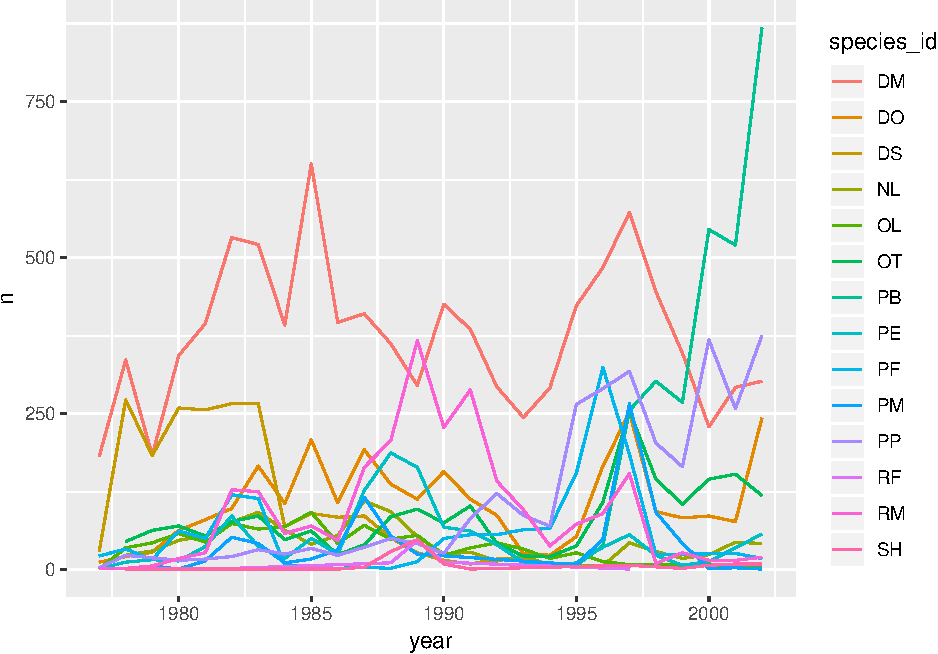
\includegraphics{img/R-ecology-time-series-with-colors-1.pdf}

\section{Faceting}\label{faceting}

\textbf{\texttt{ggplot2}} has a special technique called \emph{faceting}
that allows the user to split one plot into multiple plots based on a
factor included in the dataset. We will use it to make a time series
plot for each species:

\begin{Shaded}
\begin{Highlighting}[]
\KeywordTok{ggplot}\NormalTok{(}\DataTypeTok{data =}\NormalTok{ yearly_counts, }\DataTypeTok{mapping =} \KeywordTok{aes}\NormalTok{(}\DataTypeTok{x =}\NormalTok{ year, }\DataTypeTok{y =}\NormalTok{ n)) }\OperatorTok{+}
\StringTok{    }\KeywordTok{geom_line}\NormalTok{() }\OperatorTok{+}
\StringTok{    }\KeywordTok{facet_wrap}\NormalTok{(}\OperatorTok{~}\StringTok{ }\NormalTok{species_id)}
\end{Highlighting}
\end{Shaded}

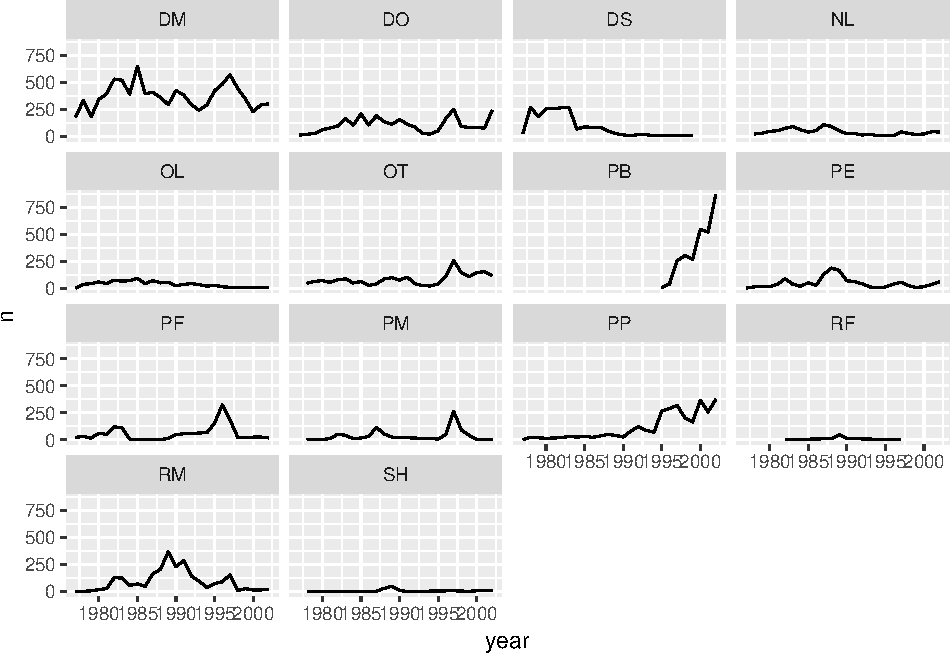
\includegraphics{img/R-ecology-first-facet-1.pdf}

Now we would like to split the line in each plot by the sex of each
individual measured. To do that we need to make counts in the data frame
grouped by \texttt{year}, \texttt{species\_id}, and \texttt{sex}:

\begin{Shaded}
\begin{Highlighting}[]
\NormalTok{ yearly_sex_counts <-}\StringTok{ }\NormalTok{surveys_complete }\OperatorTok
\StringTok{                      }\KeywordTok{count}\NormalTok{(year, species_id, sex)}
\end{Highlighting}
\end{Shaded}

We can now make the faceted plot by splitting further by sex using
\texttt{color} (within a single plot):

\begin{Shaded}
\begin{Highlighting}[]
 \KeywordTok{ggplot}\NormalTok{(}\DataTypeTok{data =}\NormalTok{ yearly_sex_counts, }\DataTypeTok{mapping =} \KeywordTok{aes}\NormalTok{(}\DataTypeTok{x =}\NormalTok{ year, }\DataTypeTok{y =}\NormalTok{ n, }\DataTypeTok{color =}\NormalTok{ sex)) }\OperatorTok{+}
\StringTok{     }\KeywordTok{geom_line}\NormalTok{() }\OperatorTok{+}
\StringTok{     }\KeywordTok{facet_wrap}\NormalTok{(}\OperatorTok{~}\StringTok{ }\NormalTok{species_id)}
\end{Highlighting}
\end{Shaded}

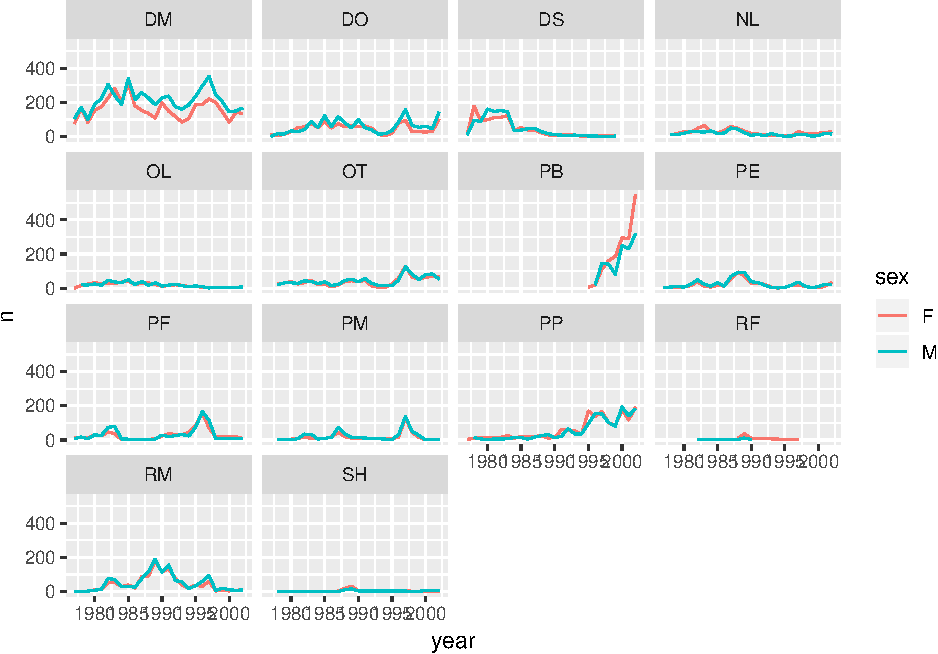
\includegraphics{img/R-ecology-facet-by-species-and-sex-1.pdf}

Usually plots with white background look more readable when printed. We
can set the background to white using the function \texttt{theme\_bw()}.
Additionally, you can remove the grid:

\begin{Shaded}
\begin{Highlighting}[]
 \KeywordTok{ggplot}\NormalTok{(}\DataTypeTok{data =}\NormalTok{ yearly_sex_counts, }\DataTypeTok{mapping =} \KeywordTok{aes}\NormalTok{(}\DataTypeTok{x =}\NormalTok{ year, }\DataTypeTok{y =}\NormalTok{ n, }\DataTypeTok{color =}\NormalTok{ sex)) }\OperatorTok{+}
\StringTok{     }\KeywordTok{geom_line}\NormalTok{() }\OperatorTok{+}
\StringTok{     }\KeywordTok{facet_wrap}\NormalTok{(}\OperatorTok{~}\StringTok{ }\NormalTok{species_id) }\OperatorTok{+}
\StringTok{     }\KeywordTok{theme_bw}\NormalTok{() }\OperatorTok{+}
\StringTok{     }\KeywordTok{theme}\NormalTok{(}\DataTypeTok{panel.grid =} \KeywordTok{element_blank}\NormalTok{())}
\end{Highlighting}
\end{Shaded}

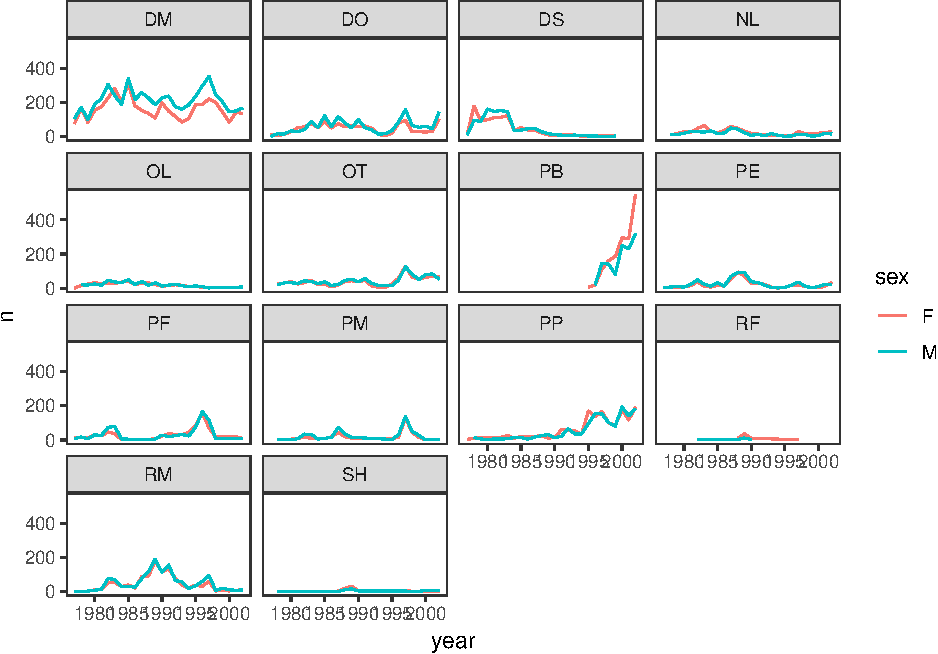
\includegraphics{img/R-ecology-facet-by-species-and-sex-white-bg-1.pdf}

\section{\texorpdfstring{\textbf{\texttt{ggplot2}}
themes}{ggplot2 themes}}\label{ggplot2-themes}

In addition to \texttt{theme\_bw()}, which changes the plot background
to white, \textbf{\texttt{ggplot2}} comes with several other themes
which can be useful to quickly change the look of your visualization.
The complete list of themes is available at
\url{http://docs.ggplot2.org/current/ggtheme.html}.
\texttt{theme\_minimal()} and \texttt{theme\_light()} are popular, and
\texttt{theme\_void()} can be useful as a starting point to create a new
hand-crafted theme.

The
\href{https://jrnold.github.io/ggthemes/reference/index.html}{ggthemes}
package provides a wide variety of options (including an Excel 2003
theme). The
\href{https://www.ggplot2-exts.org}{\textbf{\texttt{ggplot2}} extensions
website} provides a list of packages that extend the capabilities of
\textbf{\texttt{ggplot2}}, including additional themes.

\begin{quote}
\subsection{Challenge}\label{challenge-9}
\end{quote}

\begin{quote}
Use what you just learned to create a plot that depicts how the average
weight of each species changes through the years.

Answer

\begin{Shaded}
\begin{Highlighting}[]
\NormalTok{yearly_weight <-}\StringTok{ }\NormalTok{surveys_complete }\OperatorTok
\StringTok{                }\KeywordTok{group_by}\NormalTok{(year, species_id) }\OperatorTok
\StringTok{                 }\KeywordTok{summarize}\NormalTok{(}\DataTypeTok{avg_weight =} \KeywordTok{mean}\NormalTok{(weight))}
\KeywordTok{ggplot}\NormalTok{(}\DataTypeTok{data =}\NormalTok{ yearly_weight, }\DataTypeTok{mapping =} \KeywordTok{aes}\NormalTok{(}\DataTypeTok{x=}\NormalTok{year, }\DataTypeTok{y=}\NormalTok{avg_weight)) }\OperatorTok{+}
\StringTok{   }\KeywordTok{geom_line}\NormalTok{() }\OperatorTok{+}
\StringTok{   }\KeywordTok{facet_wrap}\NormalTok{(}\OperatorTok{~}\StringTok{ }\NormalTok{species_id) }\OperatorTok{+}
\StringTok{   }\KeywordTok{theme_bw}\NormalTok{()}
\end{Highlighting}
\end{Shaded}

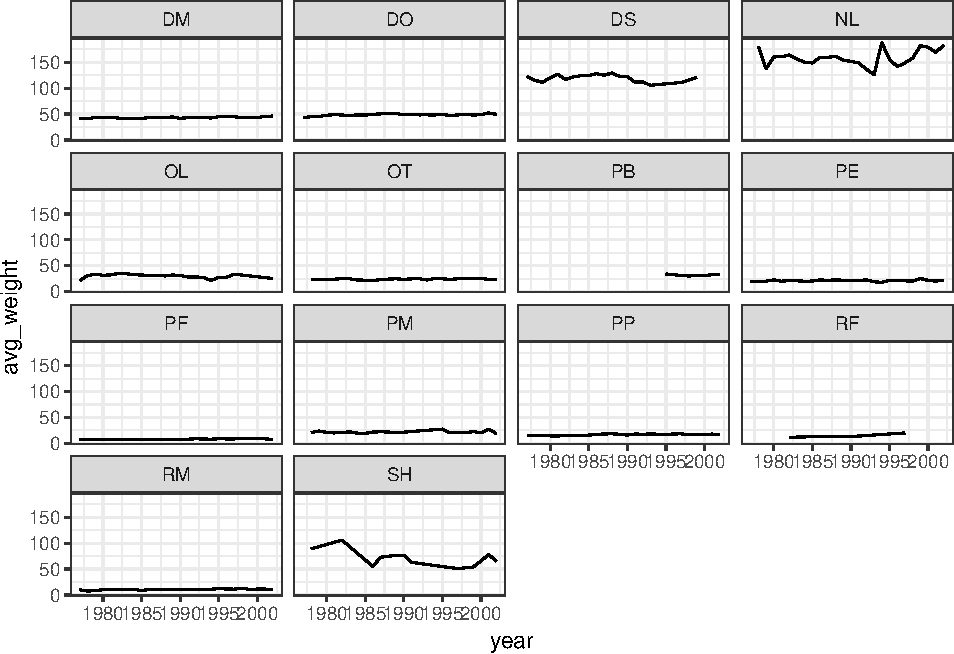
\includegraphics{img/R-ecology-average-weight-time-series-1.pdf}
\end{quote}

The \texttt{facet\_wrap} geometry extracts plots into an arbitrary
number of dimensions to allow them to cleanly fit on one page. On the
other hand, the \texttt{facet\_grid} geometry allows you to explicitly
specify how you want your plots to be arranged via formula notation
(\texttt{rows\ \textasciitilde{}\ columns}; a \texttt{.} can be used as
a placeholder that indicates only one row or column).

Let's modify the previous plot to compare how the weights of males and
females has changed through time:

\begin{Shaded}
\begin{Highlighting}[]
\CommentTok{# One column, facet by rows}
\NormalTok{yearly_sex_weight <-}\StringTok{ }\NormalTok{surveys_complete }\OperatorTok
\StringTok{    }\KeywordTok{group_by}\NormalTok{(year, sex, species_id) }\OperatorTok
\StringTok{    }\KeywordTok{summarize}\NormalTok{(}\DataTypeTok{avg_weight =} \KeywordTok{mean}\NormalTok{(weight))}
\KeywordTok{ggplot}\NormalTok{(}\DataTypeTok{data =}\NormalTok{ yearly_sex_weight, }
       \DataTypeTok{mapping =} \KeywordTok{aes}\NormalTok{(}\DataTypeTok{x =}\NormalTok{ year, }\DataTypeTok{y =}\NormalTok{ avg_weight, }\DataTypeTok{color =}\NormalTok{ species_id)) }\OperatorTok{+}
\StringTok{    }\KeywordTok{geom_line}\NormalTok{() }\OperatorTok{+}
\StringTok{    }\KeywordTok{facet_grid}\NormalTok{(sex }\OperatorTok{~}\StringTok{ }\NormalTok{.)}
\end{Highlighting}
\end{Shaded}

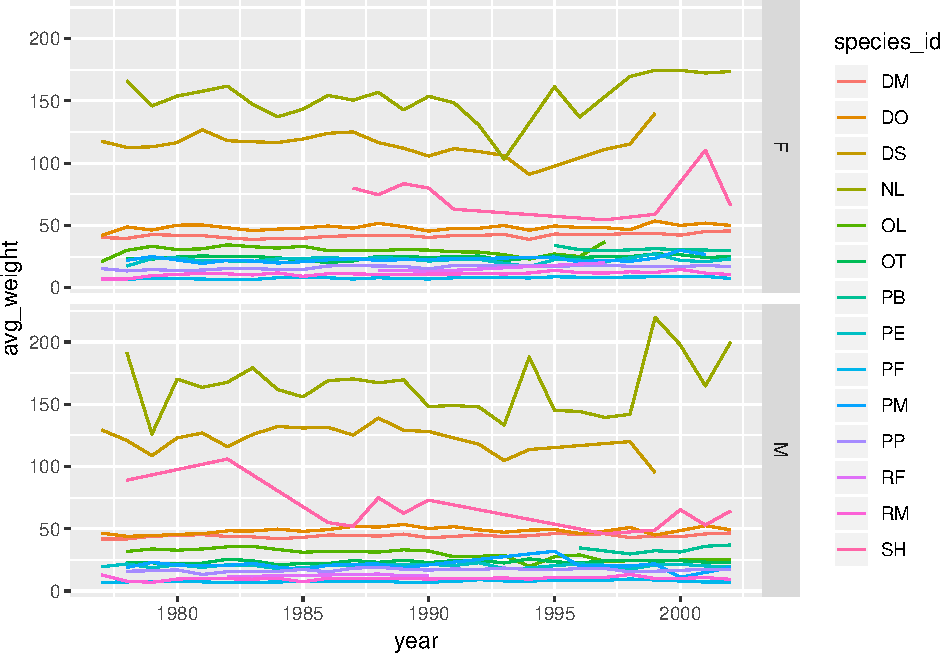
\includegraphics{img/R-ecology-average-weight-time-facet-sex-rows-1.pdf}

\begin{Shaded}
\begin{Highlighting}[]
\CommentTok{# One row, facet by column}
\KeywordTok{ggplot}\NormalTok{(}\DataTypeTok{data =}\NormalTok{ yearly_sex_weight, }
       \DataTypeTok{mapping =} \KeywordTok{aes}\NormalTok{(}\DataTypeTok{x =}\NormalTok{ year, }\DataTypeTok{y =}\NormalTok{ avg_weight, }\DataTypeTok{color =}\NormalTok{ species_id)) }\OperatorTok{+}
\StringTok{    }\KeywordTok{geom_line}\NormalTok{() }\OperatorTok{+}
\StringTok{    }\KeywordTok{facet_grid}\NormalTok{(. }\OperatorTok{~}\StringTok{ }\NormalTok{sex)}
\end{Highlighting}
\end{Shaded}

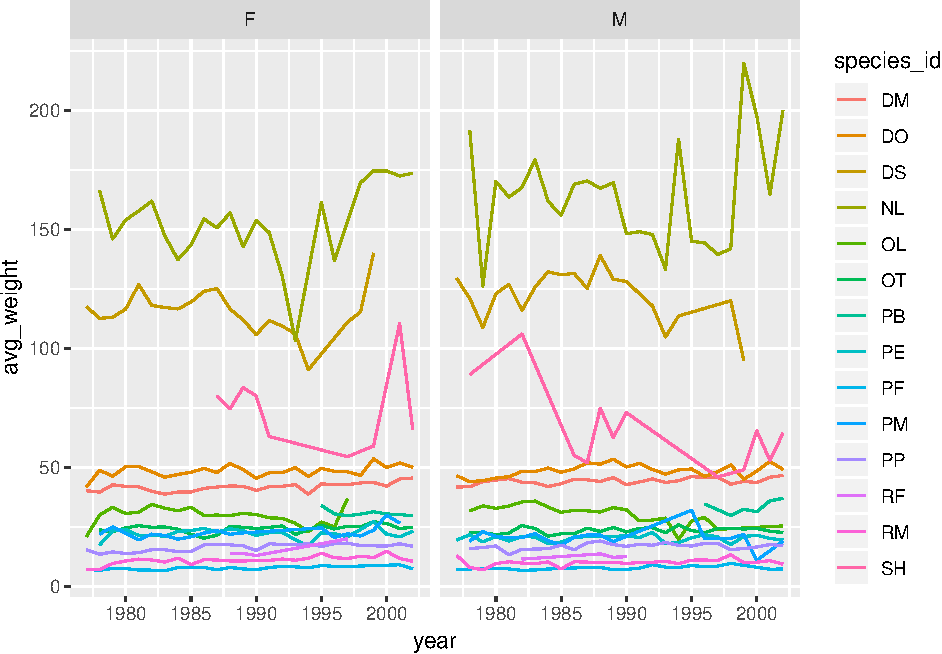
\includegraphics{img/R-ecology-average-weight-time-facet-sex-columns-1.pdf}

\section{Customization}\label{customization}

Take a look at the
\href{https://www.rstudio.com/wp-content/uploads/2016/11/ggplot2-cheatsheet-2.1.pdf}{\textbf{\texttt{ggplot2}}
cheat sheet}, and think of ways you could improve the plot.

Now, let's change names of axes to something more informative than
`year' and `n' and add a title to the figure:

\begin{Shaded}
\begin{Highlighting}[]
\KeywordTok{ggplot}\NormalTok{(}\DataTypeTok{data =}\NormalTok{ yearly_sex_counts, }\DataTypeTok{mapping =} \KeywordTok{aes}\NormalTok{(}\DataTypeTok{x =}\NormalTok{ year, }\DataTypeTok{y =}\NormalTok{ n, }\DataTypeTok{color =}\NormalTok{ sex)) }\OperatorTok{+}
\StringTok{    }\KeywordTok{geom_line}\NormalTok{() }\OperatorTok{+}
\StringTok{    }\KeywordTok{facet_wrap}\NormalTok{(}\OperatorTok{~}\StringTok{ }\NormalTok{species_id) }\OperatorTok{+}
\StringTok{    }\KeywordTok{labs}\NormalTok{(}\DataTypeTok{title =} \StringTok{"Observed species in time"}\NormalTok{,}
         \DataTypeTok{x =} \StringTok{"Year of observation"}\NormalTok{,}
         \DataTypeTok{y =} \StringTok{"Number of species"}\NormalTok{) }\OperatorTok{+}
\StringTok{    }\KeywordTok{theme_bw}\NormalTok{()}
\end{Highlighting}
\end{Shaded}

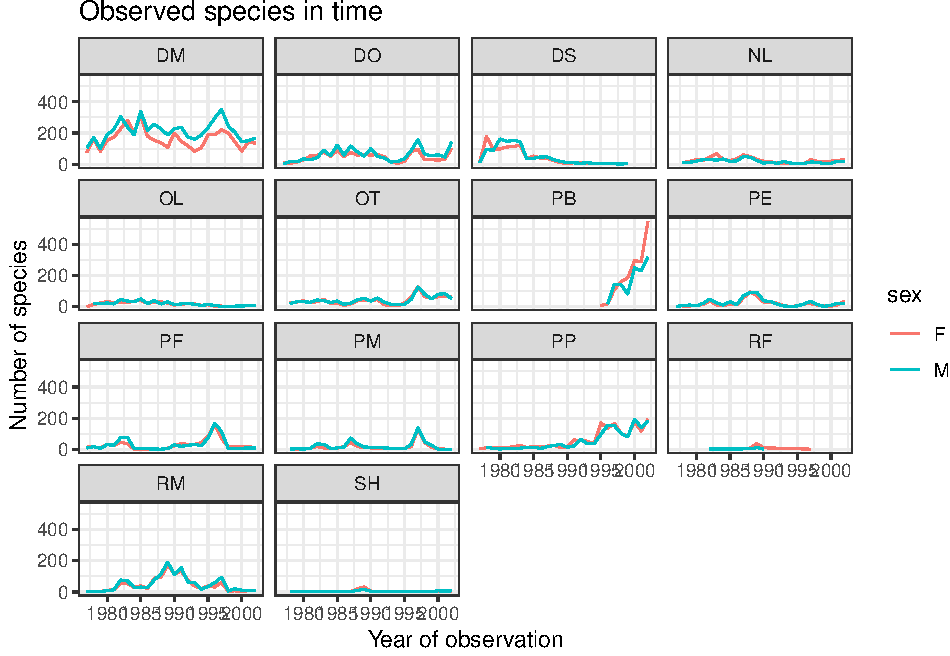
\includegraphics{img/R-ecology-number-species-year-with-right-labels-1.pdf}

The axes have more informative names, but their readability can be
improved by increasing the font size:

\begin{Shaded}
\begin{Highlighting}[]
\KeywordTok{ggplot}\NormalTok{(}\DataTypeTok{data =}\NormalTok{ yearly_sex_counts, }\DataTypeTok{mapping =} \KeywordTok{aes}\NormalTok{(}\DataTypeTok{x =}\NormalTok{ year, }\DataTypeTok{y =}\NormalTok{ n, }\DataTypeTok{color =}\NormalTok{ sex)) }\OperatorTok{+}
\StringTok{    }\KeywordTok{geom_line}\NormalTok{() }\OperatorTok{+}
\StringTok{    }\KeywordTok{facet_wrap}\NormalTok{(}\OperatorTok{~}\StringTok{ }\NormalTok{species_id) }\OperatorTok{+}
\StringTok{    }\KeywordTok{labs}\NormalTok{(}\DataTypeTok{title =} \StringTok{"Observed species in time"}\NormalTok{,}
        \DataTypeTok{x =} \StringTok{"Year of observation"}\NormalTok{,}
        \DataTypeTok{y =} \StringTok{"Number of species"}\NormalTok{) }\OperatorTok{+}
\StringTok{    }\KeywordTok{theme_bw}\NormalTok{() }\OperatorTok{+}
\StringTok{    }\KeywordTok{theme}\NormalTok{(}\DataTypeTok{text=}\KeywordTok{element_text}\NormalTok{(}\DataTypeTok{size =} \DecValTok{16}\NormalTok{))}
\end{Highlighting}
\end{Shaded}

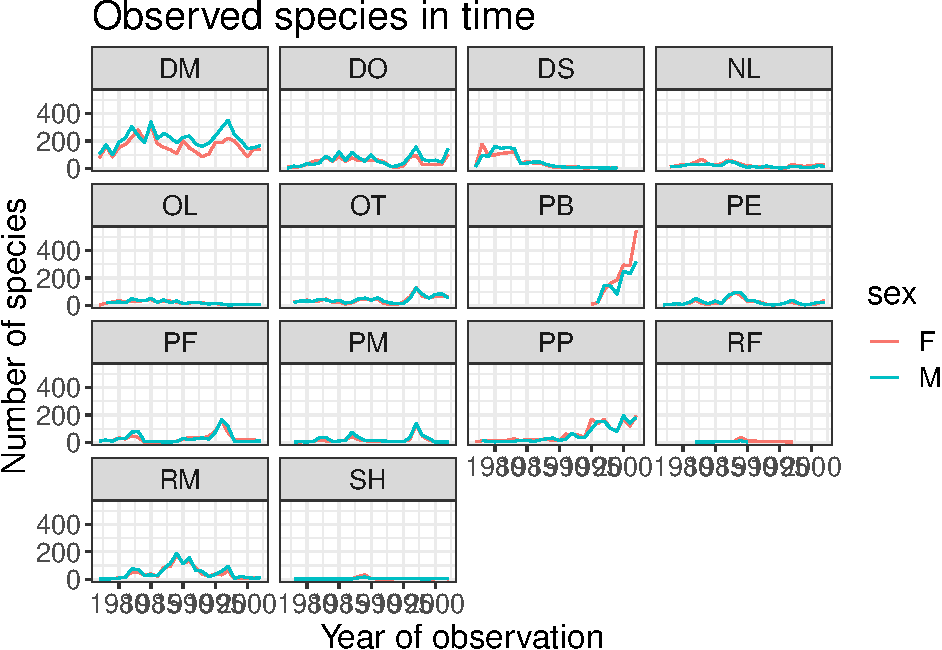
\includegraphics{img/R-ecology-number-species-year-with-right-labels-xfont-size-1.pdf}

Note that it is also possible to change the fonts of your plots. If you
are on Windows, you may have to install the
\href{https://github.com/wch/extrafont}{\textbf{\texttt{extrafont}}
package}, and follow the instructions included in the README for this
package.

After our manipulations, you may notice that the values on the x-axis
are still not properly readable. Let's change the orientation of the
labels and adjust them vertically and horizontally so they don't
overlap. You can use a 90-degree angle, or experiment to find the
appropriate angle for diagonally oriented labels:

\begin{Shaded}
\begin{Highlighting}[]
\KeywordTok{ggplot}\NormalTok{(}\DataTypeTok{data =}\NormalTok{ yearly_sex_counts, }\DataTypeTok{mapping =} \KeywordTok{aes}\NormalTok{(}\DataTypeTok{x =}\NormalTok{ year, }\DataTypeTok{y =}\NormalTok{ n, }\DataTypeTok{color =}\NormalTok{ sex)) }\OperatorTok{+}
\StringTok{    }\KeywordTok{geom_line}\NormalTok{() }\OperatorTok{+}
\StringTok{    }\KeywordTok{facet_wrap}\NormalTok{(}\OperatorTok{~}\StringTok{ }\NormalTok{species_id) }\OperatorTok{+}
\StringTok{    }\KeywordTok{labs}\NormalTok{(}\DataTypeTok{title =} \StringTok{"Observed species in time"}\NormalTok{,}
        \DataTypeTok{x =} \StringTok{"Year of observation"}\NormalTok{,}
        \DataTypeTok{y =} \StringTok{"Number of species"}\NormalTok{) }\OperatorTok{+}
\StringTok{    }\KeywordTok{theme_bw}\NormalTok{() }\OperatorTok{+}
\StringTok{    }\KeywordTok{theme}\NormalTok{(}\DataTypeTok{axis.text.x =} \KeywordTok{element_text}\NormalTok{(}\DataTypeTok{colour =} \StringTok{"grey20"}\NormalTok{, }\DataTypeTok{size =} \DecValTok{12}\NormalTok{, }\DataTypeTok{angle =} \DecValTok{90}\NormalTok{, }\DataTypeTok{hjust =} \FloatTok{0.5}\NormalTok{, }\DataTypeTok{vjust =} \FloatTok{0.5}\NormalTok{),}
                        \DataTypeTok{axis.text.y =} \KeywordTok{element_text}\NormalTok{(}\DataTypeTok{colour =} \StringTok{"grey20"}\NormalTok{, }\DataTypeTok{size =} \DecValTok{12}\NormalTok{),}
          \DataTypeTok{text =} \KeywordTok{element_text}\NormalTok{(}\DataTypeTok{size =} \DecValTok{16}\NormalTok{))}
\end{Highlighting}
\end{Shaded}

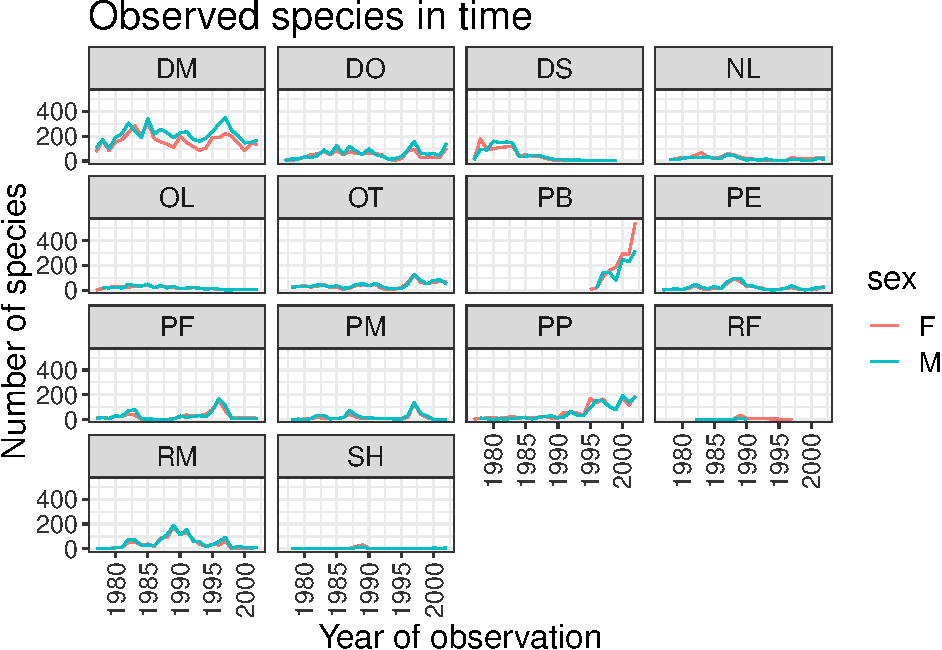
\includegraphics{img/R-ecology-number-species-year-with-theme-1.pdf}

If you like the changes you created better than the default theme, you
can save them as an object to be able to easily apply them to other
plots you may create:

\begin{Shaded}
\begin{Highlighting}[]
\NormalTok{grey_theme <-}\StringTok{ }\KeywordTok{theme}\NormalTok{(}\DataTypeTok{axis.text.x =} \KeywordTok{element_text}\NormalTok{(}\DataTypeTok{colour =} \StringTok{"grey20"}\NormalTok{, }\DataTypeTok{size =} \DecValTok{12}\NormalTok{, }\DataTypeTok{angle =} \DecValTok{90}\NormalTok{, }\DataTypeTok{hjust =} \FloatTok{0.5}\NormalTok{, }\DataTypeTok{vjust =} \FloatTok{0.5}\NormalTok{),}
                          \DataTypeTok{axis.text.y =} \KeywordTok{element_text}\NormalTok{(}\DataTypeTok{colour =} \StringTok{"grey20"}\NormalTok{, }\DataTypeTok{size =} \DecValTok{12}\NormalTok{),}
                          \DataTypeTok{text =} \KeywordTok{element_text}\NormalTok{(}\DataTypeTok{size =} \DecValTok{16}\NormalTok{))}
\KeywordTok{ggplot}\NormalTok{(surveys_complete, }\KeywordTok{aes}\NormalTok{(}\DataTypeTok{x =}\NormalTok{ species_id, }\DataTypeTok{y =}\NormalTok{ hindfoot_length)) }\OperatorTok{+}
\StringTok{    }\KeywordTok{geom_boxplot}\NormalTok{() }\OperatorTok{+}
\StringTok{    }\NormalTok{grey_theme}
\end{Highlighting}
\end{Shaded}

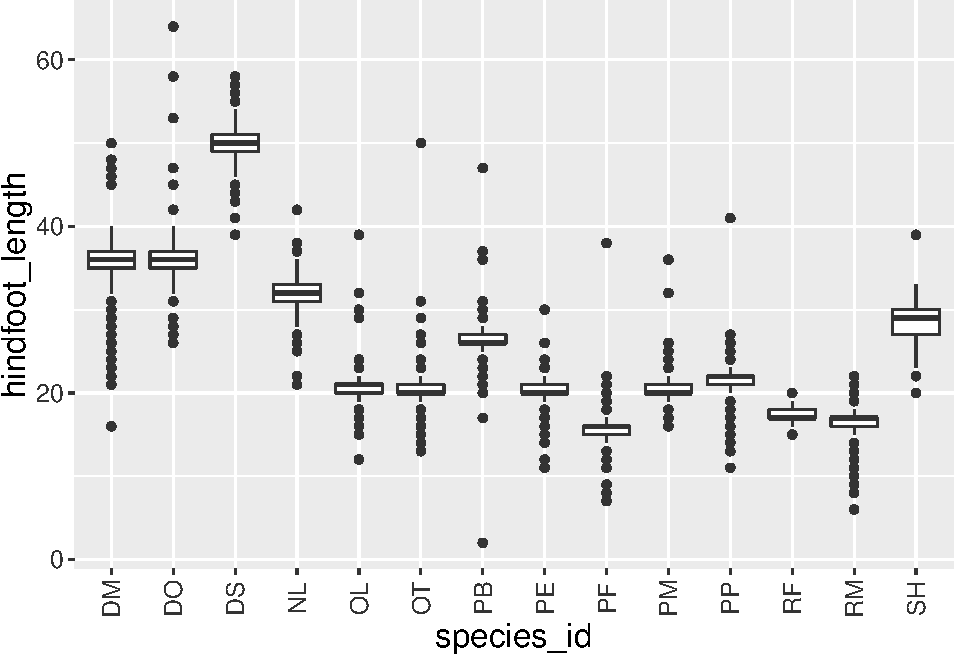
\includegraphics{img/R-ecology-number-species-year-with-right-labels-xfont-orientation-1.pdf}

\begin{quote}
\subsection{Challenge}\label{challenge-10}

With all of this information in hand, please take another five minutes
to either improve one of the plots generated in this exercise or create
a beautiful graph of your own. Use the RStudio
\href{https://www.rstudio.com/wp-content/uploads/2016/11/ggplot2-cheatsheet-2.1.pdf}{\textbf{\texttt{ggplot2}}
cheat sheet} for inspiration. Here are some ideas:

\begin{itemize}
\tightlist
\item
  See if you can change the thickness of the lines.
\item
  Can you find a way to change the name of the legend? What about its
  labels?
\item
  Try using a different color palette (see
  \url{http://www.cookbook-r.com/Graphs/Colors_(ggplot2)/}).
\end{itemize}
\end{quote}

\section{Arranging and exporting
plots}\label{arranging-and-exporting-plots}

Faceting is a great tool for splitting one plot into multiple plots, but
sometimes you may want to produce a single figure that contains multiple
plots using different variables or even different data frames. The
\textbf{\texttt{gridExtra}} package allows us to combine separate
ggplots into a single figure using \texttt{grid.arrange()}:

\begin{Shaded}
\begin{Highlighting}[]
\KeywordTok{install.packages}\NormalTok{(}\StringTok{"gridExtra"}\NormalTok{)}
\end{Highlighting}
\end{Shaded}

\begin{Shaded}
\begin{Highlighting}[]
\KeywordTok{library}\NormalTok{(gridExtra)}

\NormalTok{spp_weight_boxplot <-}\StringTok{ }\KeywordTok{ggplot}\NormalTok{(}\DataTypeTok{data =}\NormalTok{ surveys_complete, }
                             \DataTypeTok{mapping =} \KeywordTok{aes}\NormalTok{(}\DataTypeTok{x =}\NormalTok{ species_id, }\DataTypeTok{y =}\NormalTok{ weight)) }\OperatorTok{+}
\StringTok{  }\KeywordTok{geom_boxplot}\NormalTok{() }\OperatorTok{+}
\StringTok{  }\KeywordTok{xlab}\NormalTok{(}\StringTok{"Species"}\NormalTok{) }\OperatorTok{+}\StringTok{ }\KeywordTok{ylab}\NormalTok{(}\StringTok{"Weight (g)"}\NormalTok{) }\OperatorTok{+}
\StringTok{  }\KeywordTok{scale_y_log10}\NormalTok{()}

\NormalTok{spp_count_plot <-}\StringTok{ }\KeywordTok{ggplot}\NormalTok{(}\DataTypeTok{data =}\NormalTok{ yearly_counts, }
                         \DataTypeTok{mapping =} \KeywordTok{aes}\NormalTok{(}\DataTypeTok{x =}\NormalTok{ year, }\DataTypeTok{y =}\NormalTok{ n, }\DataTypeTok{color =}\NormalTok{ species_id)) }\OperatorTok{+}
\StringTok{  }\KeywordTok{geom_line}\NormalTok{() }\OperatorTok{+}\StringTok{ }
\StringTok{  }\KeywordTok{xlab}\NormalTok{(}\StringTok{"Year"}\NormalTok{) }\OperatorTok{+}\StringTok{ }\KeywordTok{ylab}\NormalTok{(}\StringTok{"Abundance"}\NormalTok{)}

\KeywordTok{grid.arrange}\NormalTok{(spp_weight_boxplot, spp_count_plot, }\DataTypeTok{ncol =} \DecValTok{2}\NormalTok{, }\DataTypeTok{widths =} \KeywordTok{c}\NormalTok{(}\DecValTok{4}\NormalTok{, }\DecValTok{6}\NormalTok{))}
\end{Highlighting}
\end{Shaded}

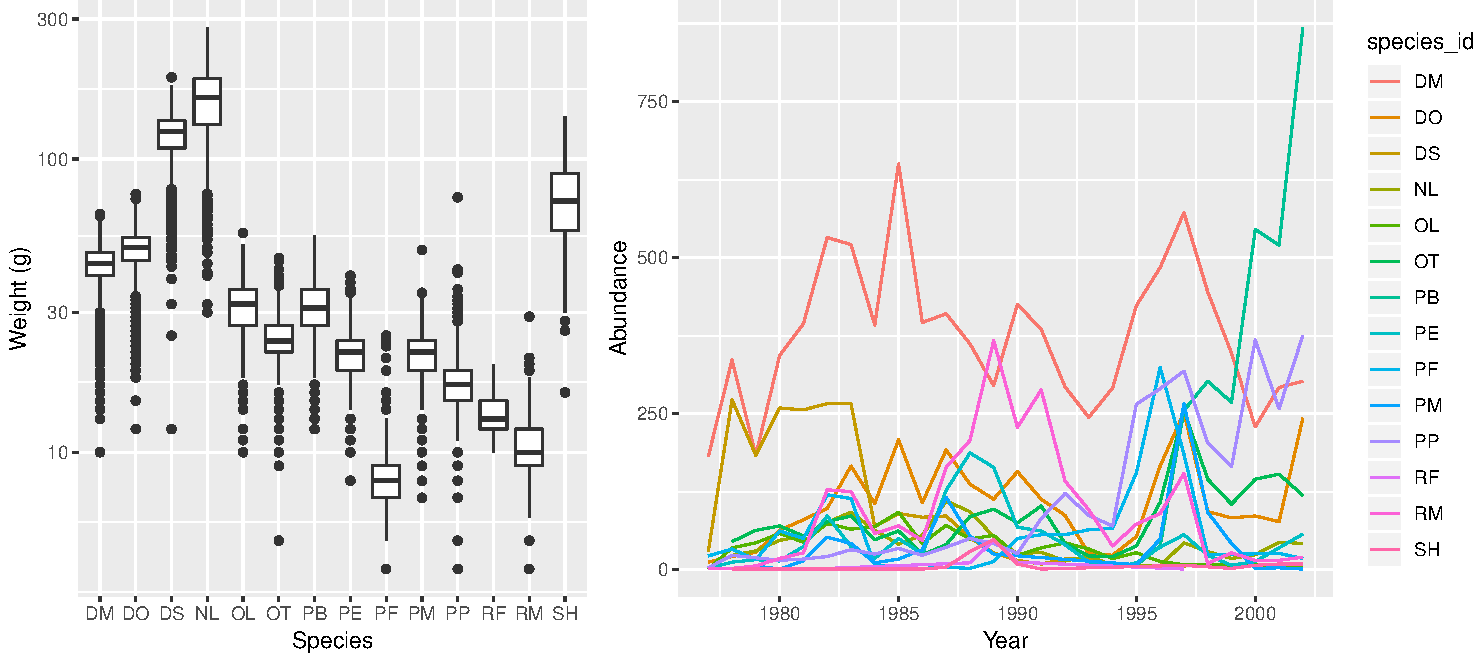
\includegraphics{img/R-ecology-gridarrange-example-1.pdf}

In addition to the \texttt{ncol} and \texttt{nrow} arguments, used to
make simple arrangements, there are tools for
\href{https://cran.r-project.org/web/packages/gridExtra/vignettes/arrangeGrob.html}{constructing
more complex layouts}.

After creating your plot, you can save it to a file in your favorite
format. The Export tab in the \textbf{Plot} pane in RStudio will save
your plots at low resolution, which will not be accepted by many
journals and will not scale well for posters.

Instead, use the \texttt{ggsave()} function, which allows you easily
change the dimension and resolution of your plot by adjusting the
appropriate arguments (\texttt{width}, \texttt{height} and
\texttt{dpi}).

Make sure you have the \texttt{fig\_output/} folder in your working
directory.

\begin{Shaded}
\begin{Highlighting}[]
\NormalTok{my_plot <-}\StringTok{ }\KeywordTok{ggplot}\NormalTok{(}\DataTypeTok{data =}\NormalTok{ yearly_sex_counts, }
                  \DataTypeTok{mapping =} \KeywordTok{aes}\NormalTok{(}\DataTypeTok{x =}\NormalTok{ year, }\DataTypeTok{y =}\NormalTok{ n, }\DataTypeTok{color =}\NormalTok{ sex)) }\OperatorTok{+}
\StringTok{    }\KeywordTok{geom_line}\NormalTok{() }\OperatorTok{+}
\StringTok{    }\KeywordTok{facet_wrap}\NormalTok{(}\OperatorTok{~}\StringTok{ }\NormalTok{species_id) }\OperatorTok{+}
\StringTok{    }\KeywordTok{labs}\NormalTok{(}\DataTypeTok{title =} \StringTok{"Observed species in time"}\NormalTok{,}
        \DataTypeTok{x =} \StringTok{"Year of observation"}\NormalTok{,}
        \DataTypeTok{y =} \StringTok{"Number of species"}\NormalTok{) }\OperatorTok{+}
\StringTok{    }\KeywordTok{theme_bw}\NormalTok{() }\OperatorTok{+}
\StringTok{    }\KeywordTok{theme}\NormalTok{(}\DataTypeTok{axis.text.x =} \KeywordTok{element_text}\NormalTok{(}\DataTypeTok{colour =} \StringTok{"grey20"}\NormalTok{, }\DataTypeTok{size =} \DecValTok{12}\NormalTok{, }\DataTypeTok{angle =} \DecValTok{90}\NormalTok{, }\DataTypeTok{hjust =} \FloatTok{0.5}\NormalTok{, }\DataTypeTok{vjust =} \FloatTok{0.5}\NormalTok{),}
                        \DataTypeTok{axis.text.y =} \KeywordTok{element_text}\NormalTok{(}\DataTypeTok{colour =} \StringTok{"grey20"}\NormalTok{, }\DataTypeTok{size =} \DecValTok{12}\NormalTok{),}
          \DataTypeTok{text=}\KeywordTok{element_text}\NormalTok{(}\DataTypeTok{size =} \DecValTok{16}\NormalTok{))}
\KeywordTok{ggsave}\NormalTok{(}\StringTok{"fig_output/yearly_sex_counts.png"}\NormalTok{, my_plot, }\DataTypeTok{width =} \DecValTok{15}\NormalTok{, }\DataTypeTok{height =} \DecValTok{10}\NormalTok{)}

\CommentTok{# This also works for grid.arrange() plots}
\NormalTok{combo_plot <-}\StringTok{ }\KeywordTok{grid.arrange}\NormalTok{(spp_weight_boxplot, spp_count_plot, }\DataTypeTok{ncol =} \DecValTok{2}\NormalTok{, }\DataTypeTok{widths =} \KeywordTok{c}\NormalTok{(}\DecValTok{4}\NormalTok{, }\DecValTok{6}\NormalTok{))}
\KeywordTok{ggsave}\NormalTok{(}\StringTok{"fig_output/combo_plot_abun_weight.png"}\NormalTok{, combo_plot, }\DataTypeTok{width =} \DecValTok{10}\NormalTok{, }\DataTypeTok{dpi =} \DecValTok{300}\NormalTok{)}
\end{Highlighting}
\end{Shaded}

Note: The parameters \texttt{width} and \texttt{height} also determine
the font size in the saved plot.

\chapter{Hakai Data Portal API}\label{hakai-data-portal-api}

Often your data source changes over time as new data are added, or as
errors are corrected. It can be a pain to go somewhere to re-download a
data file, put the data in the right place, and then re-run your code.

It is possible to download data from the Hakai EIMS Data Portal database
directly from R Studio. This is accomplished by interacting with an
application programming interface (API) that was developed for
downloading data from Hakai's data portal.

Below is a quickstart example of how you can download some chlorophyll
data. Run the code below one line at a time. When you run the
\texttt{client\ \textless{}-\ ...} line a web URL will be displayed in
the console. Copy and paste that URL into your browser. This should take
to you a webpage that displays another web URL, this is your
authentication token that permits you access to the database. Copy and
paste the URL into the console in R where it tells you to do so.

\begin{verbatim}
# Run this first line only if you haven't installedt the R API before
devtools::install_github("HakaiInstitute/hakai-api-client-r", subdir='hakaiApi')

library('hakaiApi')

# Run this line independently before the rest of the code to get the API authentication
client <- hakaiApi::Client$new() # Follow stdout prompts to get an API token

# Make a data request for chlorophyll data
endpoint <- sprintf("%s/%s", client$api_root, "eims/views/output/chlorophyll?limit=50")
data <- client$get(endpoint)

# Print out the data
print(data)
\end{verbatim}

By running this code you should see chlorophyll data in your
environment. The above code can be modified to select different datasets
other than chlorophyll and filter based on different logical parameters
you set. This is accomplished by editing the text after the ? in
\texttt{"eims/views/output/chlorophyll?limit=50"}.

The formula you set after the question mark is known as query string
filtering. To learn how to filter your data
\href{https://github.com/HakaiInstitute/hakai-api/blob/master/docs/querying-data.md}{read
this}.

To read generally about the API and how to use it for your first time
\href{https://github.com/HakaiInstitute/hakai-api/blob/master/docs/simplified-api-documentation.md\#what-is-the-hakai-api}{go
here}.

If you don't want to learn how to write a querystring yourself there is
an option to just copy and paste the querystring from the
\href{https://hecate.hakai.org/portal2/}{EIMS Data Portal}. Use the
portal to select the sample type, and dates and sites you'd like to
download as you normally would. To copy the querystring go to the top
right of the window where it says Options and click `Display API query'.
You can copy that string in to your endpoint definition in R. Just be
sure to copy that string starting from \texttt{eims/views/...},
excluding \texttt{https://hecate.hakai.org/api/} and then paste that
into the definitions of your endpoint and surround that string with
single quotes, ie:

\begin{verbatim}
endpoint <- sprintf("%s/%s", client$api_root, 'eims/views/output/chlorophyll?date>=2016-11-01&date<2018-11-20&work_area&&{"CALVERT"}&site_id&&{"KC13","MG4"}&survey&&{"KWAK","MACRO_MGEO"}&limit=-1'
\end{verbatim}

Make sure to add \&limit=-1 at the end of your query string so that not
only the first 20 results are downloaded, but rather everything matching
your query string is downloaded.

The page documenting the API usage can be found
\href{https://hakaiinstitute.github.io/hakai-api/}{here}


\end{document}
